#include<config.h>
CPS_START_NAMESPACE
\documentclass[12pt]{report}
\usepackage{epsfig}
\usepackage{times}
\title{An Introduction to Using the QCDSP Computer}
\author{B\'alint Jo\'o and Robert D. Mawhinney}
\parindent=0in
\parskip=0.1in


% importing other useful packages:
\usepackage{times}
\usepackage{fullpage}
\usepackage{graphicx}
\usepackage{longtable}
\usepackage{tabularx}
% color for the pdf links:
\usepackage{color}
\definecolor{darkblue}{rgb}{0.0,0.0,0.5}
% for conditional latex source:
\usepackage{ifthen}
% pdftex specifications, these are only included if we are using pdflatex:
\providecommand{\pdfoutput}{0}
\ifthenelse{\pdfoutput = 0}{
% Not PDF:
\usepackage{html}
\newcommand{\href}[2]{\htmladdnormallink{#2}{#1}}
}{
% PDF: hyperref for pdf with full linkages:
\usepackage[
pagebackref,
hyperindex,
hyperfigures,
colorlinks,
linkcolor=darkblue,
citecolor=darkblue,
pagecolor=darkblue,
urlcolor=blue,
%bookmarksopen,
pdfpagemode=None,
%=UseOutlines,
pdfhighlight={/I},
pdftitle={An Introduction to Using the QCDSP Computer},
pdfauthor={B\'alint Jo\'o and Robert D. Mawhinney},
plainpages=false
]{hyperref}
}


\setcounter{tocdepth}{1}
\setcounter{secnumdepth}{1}

\begin{document}
\maketitle
\tableofcontents
#include<config.h>
CPS_START_NAMESPACE
\chapter{Introduction}
These notes are an attempt at gently introducing a new
user to the QCDSP computer. It reflects my own particular
path of learning (which may or may not do me credit). 

\section{Organisation}
We begin in chapter \ref{c:HelloWorld} where we discuss
some introductory aspects of the QCDSP, including how 
to boot a QCDSP machine and how to run a simple 
{\em``Hello World''} application.

\section{Notational conventions}
Generally, when illustrating dialogue with the computer
we shall use the {\tt teletype font}. Filenames shall usually
be denoted in {\bf bold face}.

CPS_END_NAMESPACE

\chapter{Hello World}\label{c:HelloWorld}
\section{Foo or Bar?}
It is the long and honourable tradition of user guides to 
begin by a walk through example of how to get a simple program
(usually named {\bf foo.c} or {\bf bar.c} in more reputable 
texts) to run on a certain development platform. Such a program
usually does something simple like write the message {\em ``Hello World''}
to the screen. In this chapter we should like to show how to 
get such a program running on a QCDSP computer.

\section{Front End and Logging In}
The QCDSP is a parallel system that is accessible through a {\em front end}
 \ host, which is a possibly simpler, serial computer such as a Sun Workstation.

This is an accepted principle in supercomputing circles. For example,
the Thinking Machines Corporation Connection machines were often 
accessed from a Sun front end, as were some of the Elenia--Quadrics
supercomputers. Cray T3E computers often have another Cray supercomputer 
(such as a J90 or a YMP) as their front end.

It is important to point out, however, that the Connection Machine and 
Quadrics machines were true {\em back end} machines in the sense that
user programs ran on the front end Sun workstation, and the parallel hardware
was controlled entirely by the front end, usually for array operations.
The Cray and QCDSP supercomputers are different. They compute independently
of the front end. The front end however provides important services such
as a compilation environment, control to boot the parallel machines and
disk space for the data produced by the QCDSP. 

The QCDSP front end discussed in the rest of this section is a Sun
workstation running the SunOS 4 variant of the UNIX operating system.
Before being able to log in one requires an account to be set up
on the system, which should be requested from one of the systems staff
of the QCDSP collaboration\footnote{Currently Bob Mawhinney, email {\tt rdm@phys.columbia.edu}}.

\subsection{Login Procedures}
In the following example I shall use a host called 
{\em qcdhost.phys.columbia.edu}, which is the front end to two QCDSP 
boards (each containing 64 processors). The QCDSP boards are themselves
known as {\em q\_1} and {\em q\_2}. This machine 
is also the front end to some other machines of which more will be said later.

Logging in to QCDSP is done according to the standard network login procedure.
One can use {\tt telnet} to reach the host from anywhere on the Internet
although nowadays the more secure SSH login is recommended, which apart
from forwarding X-Windows connections also encrypts the network 
communications and does strict host--name resolutions. As an example I use
my current machine which is named {\em lattice2} \ to log into {\em qcdhost} \
via {\tt ssh}.

\begin{verbatim}
[bj@lattice2 bj]$ ssh bj@qcdhost.phys.columbia.edu
bj@qcdhost.phys.columbia.edu's password: 
Last login: Wed Mar 29 11:15:05 2000 from lattice2.pa.uky.
SunOS Release 4.1.4 (QCDHOST.sz) #2: Fri Nov 20 14:32:57 EST 1998
(qcdhost:/homeqs0/bj)%
\end{verbatim}

Note that the password needs to be entered at the prompt in the second
line, but, as is characteristic of UNIX the password is not echoed back to the 
terminal. If {\tt ssh} is not available one can use {\tt telnet} \ :
\begin{verbatim}
[bj@lattice2 bj]$ telnet qcdhost.phys.columbia.edu
Trying 128.59.196.11...
Connected to qcdhost.phys.columbia.edu.
Escape character is '^]'.


SunOS UNIX (qcdhost)

login: bj
password:
Last login: Wed Mar 29 11:20:05 2000 from lattice2.pa.uky.
SunOS Release 4.1.4 (QCDHOST.sz) #2: Fri Nov 20 14:32:57 EST 1998
(qcdhost:/homeqs0/bj)%
\end{verbatim}
or {\tt rlogin}:
\begin{verbatim}
[bj@lattice2 bj]$ rlogin -lbj qcdhost.phys.columbia.edu
bj@qcdhost.phys.columbia.edu's password: 
Last login: Wed Mar 29 11:25:05 2000 from lattice2.pa.uky.
SunOS Release 4.1.4 (QCDHOST.sz) #2: Fri Nov 20 14:32:57 EST 1998
\end{verbatim}
although in the latter two cases the protocols send the user
passwords over the networks unencrypted and liable to interception
by pesky hacksters worldwide. We note that when using {\em rlogin}
one ends up talking to a {\em SSH} connection at the QCDSP end.

\section{QOS and Environment Variables}
\subsection{QOS Version}
The QCDSP computer runs an operating system entitled {\em QOS}.
Numerous revisions of {\em QOS} exist with the current version at the
time of writing this note being {\em QOS 5.3.3}. A UNIX shell
environment variable, {\tt QOS\_VERS} is used to identify the version
of {\em QOS} that a given user will be using.  This environment
variable should be set automatically be the shell startup files at the
time the user logs in. In particular {\em qcdhost} supports the {\em
TC-Shell} ({\tt tcsh}) and the startup file in which  the environment 
variables are set is {\bf .cshrc}.

The toplevel {\em QOS} directory on {\em qcdhost} is

{\tt /qcdsp/sfw/qos.<version>}, 

where {\tt version} refers to the
operating system revision held by the variable {\tt QOS\_VERS}. For version
5.3.3 the relevant directory is 

{\tt /qcdsp/sfw/qos.5.3.3}\ .

\subsection{The Tartan C++ Compiler}
Another set of environmental variables that need to be set are related
to the installation of the Tartan C++ compiler. The two variables in 
my {\bf .cshrc} file at the time of writing are {\tt TC\_DIR} and {\tt TC\_BOARD}.
Currently these two variables are set to the following values:\begin{verbatim}
TC_DIR=/qcdsp/sfw/qos.<version>/usr:/usr/local/tartan/v2.1
TC_BOARD=qcdsp_v<version>
\end{verbatim}
where {\tt version} is the value of the variable {\tt QOS\_VERS}. I believe
that {\tt TC\_DIR} is a list of directories which contain subdirectories
for {\tt \#include} files, run time libraries etc. I suspect that {\tt TC\_BOARD}
identifies, which QOS operating system version interfaces the hardware
is compliant with ({\em but this is guesswork on my part. Bob, please enlighten us here}.) In any case these variables need to be set to sensible values
for code to compile, link, resolve and run successfully on the QCDSP computer.

\subsection{The QOS Toplevel Directory}
Let us now pass a cursory glance at the toplevel QOS directory.
A simple listing of files therein reveals the following directory 
contents
\begin{verbatim}
(qcdhost:/qcdsp/sfw/qos.5.3.3)%	ls
Makefile                        make.log
README                          os_03_20_00_18:36.tar.gz
announce                        plaq/
bug/                            qio/
diag/                           qio_qker/
distrib/                        qker/
example/                        rts/
include/                        usr/
lib/                            util_prog/
machines/
\end{verbatim}

Currently for us the most interesting of these are going to be 
the subdirectories called {\tt machines} and {\tt usr}. In the
former are defined the various machine partitions available, whereas
in the latter reside some useful header files describing the
parallel programming communications objects.

Looking at the machines directory reveals the following list:
\begin{verbatim}
(qcdhost:/qcdsp/sfw/qos.5.3.3)%	cd machines/
(qcdhost:/qcdsp/sfw/qos.5.3.3/machines)% ls
Makefile      cc_1/         q4_1/          q6_2/          q_1/
c4_1/         cc_2/         q4_2/          q7_1/          q_2/
c4_2/         cc_3/         q5_1/          q7_2/          src/
cb_2/         q3_1/         q5_2/          q8_1/
cb_3/         q3_2/         q6_1/          q8_2/
\end{verbatim}

Each directory with the exception of {\tt src} refers to a QCDSP processor
partition. We are qoing to use machines {\tt q\_1} and {\tt q\_2} for the 
rest of this guide so let us examine {\tt q\_1}:
\begin{verbatim}
(qcdhost:/qcdsp/sfw/qos.5.3.3/machines/q_1)% ls
boot_n0_notest.qrb      notest.qrb              q_1_sec4/
boot_n0_notest_25.qrb   notest_25.qrb           q_1_sec5/
debug.qrb               q_1@                    q_1_sec6/
debug_25.qrb            q_1_pri0/               standard.qrb
debug_notest.qrb        q_1_sec1/               standard_25.qrb
debug_notest_25.qrb     q_1_sec2/
dev                     q_1_sec3/
\end{verbatim}

Most of the files in this directory have the suffix {\bf .qrb}. 
These files are the configuration files for booting the QCDSP computer.
They specify which operating systems kernels are to be sent to the
QCDSP daughterboards, what speed the inter processor communications 
should run at, what self test procedures to carry out at boot time, {\em etc}\ .
In normal usage, the file {\bf standard.qrb} should probably be used
(the manner of its use will be described in the next section).

The file {\bf q\_1} is a symbolic link to a program called the 
{\em QC-Shell}, which is the shell environment used to boot, and 
run programs on the QCDSP, of which we shall say more below.

\section{The QC-Shell and Booting the QCDSP}
\subsection{The QC-Shell -- {\tt qcsh}}
So far we have been happily romping around the filesystem of the 
front end host. Now comes the time to actually boot a set of processors
for our use.

Interaction with the QCDSP generally takes place through the aforementioned
{\em QC-Shell}. This effectively is the usual {\em TC-Shell} \ with some 
bolted on features (in the form of built in commands) to manipulate the 
QCDSP computer. Commands for manipulating the QCDSP begin with the letter
{\tt q}. Some useful commands which we shall be using later are 
{\tt qreset\_boot}, {\tt qrun} and {\tt qprintf}. 

We note the distinction between a shell built in command and UNIX
commands. For example in a normal UNIX {\em TC-Shell} \ the command
{\tt echo} is a built in command of the shell, while the usual
UNIX command {\tt ls} is an executable program usually residing in
the directory {\tt /bin}.  Hence the command {\tt ls} is available to
all shells, whereas the command {\tt echo} is shell specific (although
it is implemented in almost all UNIX shells). 

Like most UNIX--shell like shells the {\em QC-Shell} \ allows for
self initialisation through a startup file. In the case of the {\em
QC-Shell} this file is called {\bf .qcshrc}. If your account has been
set up properly you should find a {\bf .qcshrc} file in your toplevel
homedirectory. My one reads as follows:
\begin{verbatim}
source ~/.cshrc
qinit
set curdir = `pwd`
source $curdir/dev
qset_qd_verbose 2
qset_qd_scsi_tree_verbose 2
qset_reset_boot f standard.qrb
qset_exit_info 5 exit.info
qreset_boot
\end{verbatim}

One of the chief functions of the {\bf .qcshrc} file is to boot the 
QCDSP computer. This is accomplished by various commands in the 
{\bf .qcshrc} file. 

The {\tt qinit} command initialises the QCDSP system and starts up
the {\tt Qdaemon} system daemon which is responsible for for booting
the QCDSP machine, loading and executing programs, performing self tests
and other important tasks.  By ``sourcing''
the {\bf dev} file in the current directory, several variables are 
defined in the shell specifying amongst other things the boot--debug
network device (in this case SCSI ID) which is used to communicate
with the QCDSP boards. {\bf Note that this .qcshrc expects you to be
in the correct machine directory at the time of invocation of the 
QC-Shell, where the file dev resides}.

Thereafter some boot time verbosity levels are set to specify how 
much of the various Qdaemon messages and other test results should be sent
to the standard output for boot time diagnostic purposes. These levels 
are set by the {\tt qset\_qd\_verbose} and the 
{\tt qset\_qd\_scsi\_tree\_verbose} 
commands.

The configuration ({\bf .qrb}) file to use when booting, or resetting
the QCDSP is specified with the command {\tt qset\_reset\_boot}. In
my case it is the {\bf standard.qrb} file which was mentioned in the
last section. 

The {\tt qset\_exit\_info} command itself is used to {\em what's it 
used to do then ?} 

Once all these settings have been put into effect the machine is 
finally booted through the command {\tt qreset\_boot}. Incidentally
this is also a useful bail out command. Should the QCDSP crash or deadlock,
or for whatever reason we may want to reboot the computer, it can be 
done using the {\tt qreset\_boot} command in the {\em QC-Shell}.

More information on these commands will be given in the
advances stages of this manual (if it ever gets that far...)

\section{Booting the QCDSP}
Now that we have examined how one boots the QCDSP, let us do it
by invoking the {\em QC-Shell}. The magic incantation for machine {\em q\_1}
is:
\begin{verbatim}
(qcdhost:/homeqs0/bj)% cd /qcdsp/sfw/qos.5.3.3/machines/q_1
(qcdhost:/qcdsp/sfw/qos.5.3.3/machines/q_1)% ./q_1
\end{verbatim}

The first command takes to the machine directory, where the {\bf dev}
and {\bf .qrb} files live. Recalling that {\tt q\_1} is a symbolic link
the {\tt qcsh} command, it can be seen that the second command invokes
the {\em QC-Shell}.

{\bf Aside: }
Since getting to the correct machine directory involves a lot of typing
it might be useful to set up some sort of shell alias to allow us
reaching the directory more quickly. In my {\bf \~\/.cshrc} file I have 
two variables set:
\begin{verbatim}
set q_1 = /qcdsp/sfw/qos."$QOS_VERS"/machines/q_1
set q_2 = /qcdsp/sfw/qos."$QOS_VERS"/machines/q_2 
\end{verbatim}
Hence I can reach the {\em q\_1} and {\em q\_2} directories respectively
by just typing {\tt cd q\_1} and {\tt cd q\_2} respectively.

The invoking of the {\em QC-Shell} should start a large set of messages
scrolling up your screen, giving you the results of boot time diagnostics
and self tests. Some important ones to look out for:
\begin{verbatim}
qinit:  qcsh initialized

Qdaemon state is:
        qdaemon task is INITIALIZE_DAEMON
        qdaemon abort no and resume no
        QCDSP not synchronous
        SCSI tree coordinates selected:  mb 0,  db 0,  
        Load address 0 (hex), data 0 (hex) from screen
        Read address (hex) 0, blksize 0 (hex) from screen
        Read output to screen in node tagged format
        Run entry address from file
        SCSI packet and payload size:  512  488
        Run kernels not installed on all nodes
        Hardware debugging level is 0
        Not decoding packet headers
\end{verbatim}
This message signifies that the {\em QC-Shell} has been initialized
and the so called {\tt Qdaemon} has been started. The {\tt Qdaemon}
is the primary source of interaction with the QCDSP. Note also 
the {\tt Qdaemon} message has been displayed twice, once for entry 
into the specific service routine and once at the exit. This is the 
result of setting the verbosity level in the {\bf .qcshrc} file.
Carrying on with the boot process the following messages should appear
at some point:
\begin{verbatim}
qset_boot_szdevice: /dev/rsz8 open
qset_boot_szdevice:  status directory /qcdsp/machines/status/qcdhost.rsz8
qdaemon verbose level: 2
SCSI tree verbose level: 2
        exit info level and filename:  5   exit.info
Qdaemon:  PRIMARY Q-SHELL - hardware reset enabled
Qdaemon:  pause between unsuccessful SCSI bus reads is 10000 microseconds

Qdaemon state is:
        qdaemon task is RESET_BOOT
        qdaemon abort no and resume no
        QCDSP not synchronous
        SCSI tree coordinates selected:  mb 0,  db 0,  
ResetBoot::ResetBoot:  Hello
\end{verbatim}
These messages show the results of trying to talk via
the SCSI bus to the QCDSP, in particular that the SCSI bus has been 
found and that the Qdaemon has now entered the machine reset and boot
service. If all is well the QCDSP should reply as:
\begin{verbatim}
Szm::inquiry:   COLUMBIA QCDSP
ResetBoot::ResetBoot:  Mb 0 found
ResetBoot:  Working on scsi layer 0
ResetBoot:  turning off LED's on layer 0
ResetBoot:  starting non SCU NGA setup on layer 0
ResetBoot:  starting DramStdTest0 on layer 0
ResetBoot:  DramStdTest0 passed for layer 0
ResetBoot:  loading run kernels to layer 0
\end{verbatim}
If you do not get the {\tt COLUMBIA QCDSP} message then
something is wrong. The rest of the messages display various test 
results.

The various motherboards are arranged in a tree structure with
boot time communication being done via a SCSI bus. One of the
next tasks of the boot process is to find out about the SCSI tree.
This information is also echoed back at boot time (given the verbosity
levels in my startup files):
\begin{verbatim}
SCSITree:  Summary of SCSITree object

  SCSIPath information for motherboard 0
    SCSI ID path:       
    SCSI branch path:   

  SCSIBranch information for branch 0

  SCSIBranch:  information for branch 0

    For SCSI ID 0 the device is motherboard 0 (serial number 38)
        at slot 0 and crate 0xf1

    For SCSI ID 1  no device is present

    For SCSI ID 2  no device is present

    For SCSI ID 3  no device is present

    For SCSI ID 4  no device is present

    For SCSI ID 5  no device is present

    For SCSI ID 6  no device is present

    For SCSI ID 7  no device is present

  SCSILayer information for layer 0
    SCSILayer:  Motherboards in this layer
          0
\end{verbatim}
Hence we see that in booting {\em q\_1} there is only one motherboard
on SCSI Id 0.

The machine then proceeds to boot all the daughter boards in turn.
This is done by sending boot kernels to all the daughter boards. 
Useful messages to look out for are 
\begin{verbatim}
DSPSerialInit:  getting information for all motherboards
DSPSerialInit:  All MB's responded with no errors

DBBoot:  Booting all Db's on all Mb's
        All nodes 1 to 63 on MB   0 booted and responded
DBBoot:  All MB's responded after Db boot
ResetBoot:  finished send of boot kernels to dbs

DSPSerialInit:  getting information for all motherboards
DSPSerialInit:  All MB's responded with no errors

DSPSerSwitchTest:  Starting to check status for all motherboards
        Network switched over all routes 10 times.
        Maximum of 10 reads done to clear receive buffer
        Mb   0 passed test
DSPSerSwitchTest:  All requested MB's responded.
        All DSP serial connections OK.
\end{verbatim} 
that show that all the motherboards and daughterboards booted OK and 
that the serial connections have been checked and are responding.
If the machine gets this far, the boot kernels boot the node gate
arrays (NGA-s) and perform a DRAM memory test. If this succeeds
the runtime kernels are downloaded to the daughterboards as 
evidenced by messages such as:
\begin{verbatim}
ResetBoot:  starting NGA boot for dbs
ResetBoot:  finished NGA boot for dbs
ResetBoot:  starting DRAM stdtest for dbs
	Checking DRAM stdtest for dbs on Mb 0
ResetBoot:  DRAM Stdtest on all dbs passed
ResetBoot:  loading run kernels to dbs
\end{verbatim}
Finally the machine is synchronised and the Serial Communications
are set up. At this point some communications tests are performed
(even and odd wire tests). Healthy messages look along the lines
of
\begin{verbatim}
ResetBoot::SCUSetup:  Beginning SCU setup of all nodes
ResetBoot::Sync:  Beginning to synchronize QCDSP
ResetBoot::Sync:  Checking that all nodes have sync set
ResetBoot::Sync:  QCDSP synchronous
ResetBoot:  running even wire send SCU test 

ResetBoot:  running odd wire send SCU test 

ResetBoot:  SCU test passed
ResetBoot::InitNodeStat:  starting send of NodeStat
ResetBoot::InitNodeStat:  starting build of NodeTable
NodeTable::NodeTable:  constructor invoked for 1 motherboards
ResetBoot::InitNodeStat:  NodeTable complete
\end{verbatim}

Finally if all goes well the Qdaemon will report that it has exited
the boot service by the message
\begin{verbatim}
Qdaemon state is:
        qdaemon task is RESET_BOOT
        qdaemon abort no and resume no
        QCDSP synchronous
        SCSI tree coordinates selected:  mb 0,  db 0,  
\end{verbatim}
and the {\em QC-Shell} will likewise show its status message
\begin{verbatim}
qcsh after RESET_BOOT:
	All nodes selected with SCSI tree coordinates
\end{verbatim}
and the {\bf boot process is complete}. Your shell prompt should
turn into something along the lines of 
\begin{verbatim}
(qcdhost/qcdsp/sfw/qos.5.3.3/machines/q_1: qcsh[q_1])% 
\end{verbatim}

Congratulations! You have now booted a QCDSP supercomputer.
Some things to be aware of
\begin{itemize}
\item
The {\em QC-Shell} does not really like lots of processes going on in parallel.
Recall that it is designed to interact with the QCDSP. This shell really
should be run only to submit QCDSP jobs. Compiling, editing, e--mailing
and the like should be carried out from the usual login {\em TC-Shell}.
\item
While in the {\em QC-Shell} you are blocking everyone else's access to a potential
HPC resource. (From a 3.2Gflop board up to a Tflops scale supercomputer.)
Spend your time in it wisely.
\item
If things become messy you can always type {\tt qreset\_boot} to reboot
the system.
\end{itemize}

\section{Hello World} 
\subsection{Compiling the Program}
The time has now come to execute the {\em Hello World}\ application.
The easiest method is to take a copy from the directory of programming
examples. You can do this by typing:
\begin{verbatim}
(qcdhost:/homeqs0/bj)% cd /qcdsp/sfw/qos.5.3.3/example/
(qcdhost:/qcdsp/sfw/qos.5.3.3/example)% tar cf - hello_world | ( cd ; tar xvf - )
x hello_world/Makefile, 608 bytes, 2 tape blocks
x hello_world/main.C, 1233 bytes, 3 tape blocks
x hello_world/hello_world.ctl, 188 bytes, 1 tape blocks
x hello_world/main.tof, 3076 bytes, 7 tape blocks
x hello_world/main.lst, 2113 bytes, 5 tape blocks
x hello_world/hello_world.map, 14453 bytes, 29 tape blocks
x hello_world/hello_world.outtof, 15276 bytes, 30 tape blocks
x hello_world/hello_world.out, 14654 bytes, 29 tape blocks
\end{verbatim}
This should copy the {\bf hello\_world} directory to your homedirectory.
A nice makefile has been provided so that we can build the application
by executing the commands:
\begin{verbatim}
(qcdhost:/homeqs0/bj)% cd hello_world/
\end{verbatim}
to go to the source directory and then:
\begin{verbatim}
(qcdhost:/homeqs0/bj/hello_world)% make clean
\end{verbatim} 
to remove the currently built stuff so we can do a clean 
rebuild. The computer should respond with 
\begin{verbatim}
rm -f  *.tof *.lst *.map core *.qin *.out *.outtof *.ctl \ .
\end{verbatim}
We perform the build by using the command {\tt make}\ :
\begin{verbatim}
(qcdhost:/homeqs0/bj/hello_world)% make
\end{verbatim}
to which the computer should reply:
\begin{verbatim}
tcpp -c -mb -km -kc -kl -q main.C
tcpp  -e hello_world.outtof -mb -km -kc -kl -q main.tof  \
   tcio30bs.olb 
Tartan Linker for QCDSP version 5.3.2, modified 1/11/99 by RDM
Memory = 0x80000, stack = 0x1000, heap = 0x1000

(See transcript written on "/homeqs0/bj/hello_world/hello_world.map"
for additional information.)
t2c hello_world.outtof hello_world.out
\end{verbatim}
In the first line, the {\tt make} system instructs the
Tartan C++ {\tt tcpp} compiler to compile the source file {\bf main.C}
which is the source for the actual {\em hello\_world} application. The second
invocation of {\tt tcpp} links the result of the compilation with the run time 
system to produce a file in the common object format. Finally the {\tt t2c}
command creates an executable format suitable for the QCDSP. The QCDSP 
executable is the one called {\bf hello\_world.out}.

\subsection{Running The Application}
Once the application has been built, it should be run.
First boot the QCDSP. This time around we will use machine {\em q\_2}.
\begin{verbatim}
(qcdhost:/homeqs0/bj/hello_world)% cd /qcdsp/sfw/qos.5.3.3/machines/q_2
(qcdhost:/qcdsp/sfw/qos.5.3.3/machines/q_2)% ./q_2
\end{verbatim}
after booting has completed we get the prompt:
\begin{verbatim}
(qcdhost/qcdsp/sfw/qos.5.3.3/machines/q_2: qcsh[q_2])% 
\end{verbatim}

To run the {\tt hello\_world} application we use the {\tt qrun} 
command:
\begin{verbatim}
(qcdhost/qcdsp/sfw/qos.5.3.3/machines/q_2: qcsh[q_2])% cd ~/hello_world/
(qcdhost/homeqs0/bj/hello_world: qcsh[q_2])% qrun hello_world.out
\end{verbatim}
The results should be a bunch of {\tt Qdaemon} messages,
indicating that the executable is being loaded to the 
QCDSP, followed by the output from Motherboard 0,
daughterboard 0:
\begin{verbatim}
Hello world
Motherboard and daughterboard numbers for this node:  0 0
Unique ID for this node:  0
Physics coordinates for this node:  0, 0, 0, 0
The square of 0 is 0
The square of 1 is 1
The square of 2 is 4
The square of 3 is 9
The square of 4 is 16
The square of 5 is 25
The square of 6 is 36
The square of 7 is 49
The square of 8 is 64
The square of 9 is 81
\end{verbatim}
followed by various exit information messages.

The output of node 0 (Motherboard 0, Daughterboard 0) is always
echoed to the standard output. The output of other nodes are 
saved to various buffers on the nodes. We can retrieve the saved
output from the processors using the {\tt qprintf} command, which
sends the saved messages to the standard output. After some Qdaemon
messages the results should look like
\begin{verbatim}
Qdaemon state is:
        qdaemon task is PRINTF
        qdaemon abort no and resume no
        QCDSP synchronous
        All nodes selected with SCSI tree coordinates

Qdaemon:  user print buffer for Mb 0 and Db 0 (SCSI tree coordinates)
Buffer wrap count 0

Hello world
Motherboard and daughterboard numbers for this node:  0 0
Unique ID for this node:  0
Physics coordinates for this node:  0, 0, 0, 0
The square of 0 is 0
The square of 1 is 1
The square of 2 is 4
The square of 3 is 9
The square of 4 is 16
The square of 5 is 25
The square of 6 is 36
The square of 7 is 49
The square of 8 is 64
The square of 9 is 81

Qdaemon:  user print buffer for Mb 0 and Db 1 (SCSI tree coordinates)
Buffer wrap count 0

Hello world
Motherboard and daughterboard numbers for this node:  0 1
Unique ID for this node:  1
Physics coordinates for this node:  0, 0, 0, 1
The square of 0 is 0
The square of 1 is 1
The square of 2 is 4
The square of 3 is 9
The square of 4 is 16
The square of 5 is 25
The square of 6 is 36
The square of 7 is 49
The square of 8 is 64
The square of 9 is 81
\end{verbatim} 
and so on for all the processors on the machine.

Congratulations! If you have followed all that I detailed here you
have now wasted the computer time of a 3.2GFlop peak speed development
board to print ``Hello World'' and some squares of numbers on the screen.

\subsection{Exiting QCDSP}
To exit fromt the QCDSP simply logout of the {\em QC-Shell} by typing
{\tt exit}.

\section{Summary}
After discussing logging in to the QCDSP system. I said a few introductory
remarks about QOS and the environmental variables needed in the shell
to be able to use QCDSP properly. I then described the boot process for the
machine. Finally I have gone through the process of building the example
{\em Hello\_World} \ application, running it and retrieving the standard
output from the various QCDSP processor buffers to where they were saved.

This is the minimal subset of knowledge needed to be able to write and
execute programs on the QCDSP computer.

\subsection{QOS and Shell Environment Summary}
The login startup files should set the environmental variables {\tt QOS\_VERS}
, {\tt TC\_DIR} and {\tt TC\_BOARD}. The current QOS version at the time
of writing this document is version 5.3.3.

The toplevel QOS directory is {\tt /qcdsp/sfw/qos.<version>}. The 
available machine partitions are in {\tt /qcdsp/sfw/qos.<version>/machines}.
The QCDSP specific include files are in {\tt /qcdsp/sfw/qos.<version>/usr/include} and the QCDSP run time libraries are in {\tt /qcdsp/sfw/qos.<version>/usr/lib}, where {\tt version} is the value held in the {\tt QOS\_VERS}.

\subsection{Booting Summary}
Go to the relevant machine directory, and invoke the {\em QC-Shell} using
the symbolic link provided (usually the same as the machine name). To use
machine {\em q\_2} for example the incantation is 
\begin{verbatim}
(qcdhost:/homeqs0/bj)% cd /qcdsp/sfw/qos.5.3.3/machines/q_2
(qcdhost:/homeqs0/bj)% ./q_2
\end{verbatim}
The machine should then boot if all goes well.

\subsection{Compilation Summary} 
Currently we did not detail compilation. We simply used the 
makefiles provided, which set the required compilation flags,
and performed the linking. We recommend copying these makefiles
for now. 

The compiler is named {\tt tcpp}, which is the Tartan C++ compiler.
There is also a utility {\tt t2c} which turns the output of the 
compilation and linking into an executable suitable for the QCDSP.
The QCDSP executables produced by the makefile have the {\bf .out}
suffix.

\subsection{Running Summary}
Once the executable has been built, it can be run using the {\tt qrun}
command. The output from processor 0 (Motherboard 0, Daughterboard 0),
is automatically echoed to the standard output. The saved standard output
buffers from the QCDSP processors can be retrieved to the standard output
of the front end host using the {\tt qprintf} command. 

\subsection{Miscalleny}
The QCDSP computer can be reset with the {\tt qreset\_boot}. The 
QCDSP machine can be freed up for others by simply logging out of 
the {\em QC--Shell}\ using the {\tt exit} command.

This concludes the ``Hello World'' chapter. In the next chapter
we shall discuss interprocessor communications.

\chapter{Basic Programming of the QCDSP}
\section{Introduction}
This chapter is intended as a guide to the basic
system calls implemented on the QCDSP computer.

The QCDSP itself is most simply programmed in C or 
C++, for which a commercial compiler exists with
some optimisation features. The compiler is called
the Tartan C++ compiler and the UNIX invocation of it 
is via the command {\tt tcpp}. 

The machine can also be programmed at the assembler
level and  indeed such programming may be necessary to achieve
maximal computational and communication performance. However,
for the moment we shall not discuss this mode of programming. 

\section{Parallelism in the QCDSP Computer}
The QCDSP, whether at the level of a single development board
or at the level of several cabinets containing processor boards
is a MIMD\footnote{Multiple Instruction Multiple Data} parallel computer. 

This means, that each processor is capable of running completely
independent code. However, the machine is 
perhaps best programmed according to the SPMD\footnote{Single Program Multiple Data} programming model. In this programming model processors run the 
same program, using different datasets resident to each processor. Also
this programming model allows one to write fully MIMD programs, by executing
separate subroutines (of the same program) depending on some identification
token (a unique processor ID, processor grid coordinates or some such) 
from the local processor. 

Furthermore, the QCDSP has a distributed memory, with no current
implementation of a shared memory system. The preferred method of 
communication is via message passing between neighbouring processors.
We shall outline possible methods to implement global communications
such as broadcasts and global sums in the next chapter.
For the current chapter, we shall introduce some of the QCDSP system
calls to allow a given particular processor to identify itself, and 
to send messages to its neighbours. To make the discussion clearer,
we have to mention a few details about the architecture and network
topology of the QCDSP computer.

\section{Brief description of the QCDSP Architecture}
The QCDSP at the bottom level consists of a collection of Texas
Instruments TMS320C31 Digital Signal Processors (DSPs) with associated
DRAM memory (0.5Gwords of error correcting memory per processor) and
special purpose communications hardware. These components are
organised into a hierarchy of {\em daughterboards}, {\em motherboards}
and {\em crates}.

A daughterboard consists of a single DSP chip, its associated DRAM and 
its so called Node Gate Array (NGA), which is the communications unit
built on a custom chip. A single daughterboard is about the size of a 
credit card. A picture of a daughterboard is shown in figure \ref{f:daughterBoard}
\begin{figure}[ht]
\begin{center}
\leavevmode
\hbox{%
\includegraphics{daughterboard_photo}
}
\end{center}
\caption{Photograph of a daughterboard. The DSP chip and the NGA are shown
with a ruler to indicate size in inches}
\label{f:daughterBoard}
\end{figure}

The daughterboards are themselves mounted on motherboards. A single
motherboard holds up to 64 daughterboards. Of these, one daughterboard
(daughterboard 0) is integrated onto the motherboard and has some 
special functions that we shall describe later. A picture of a motherboard 
can be seen in figure \ref{f:motherBoard}.

\begin{figure}[ht]
\begin{center}
\leavevmode
\hbox{%
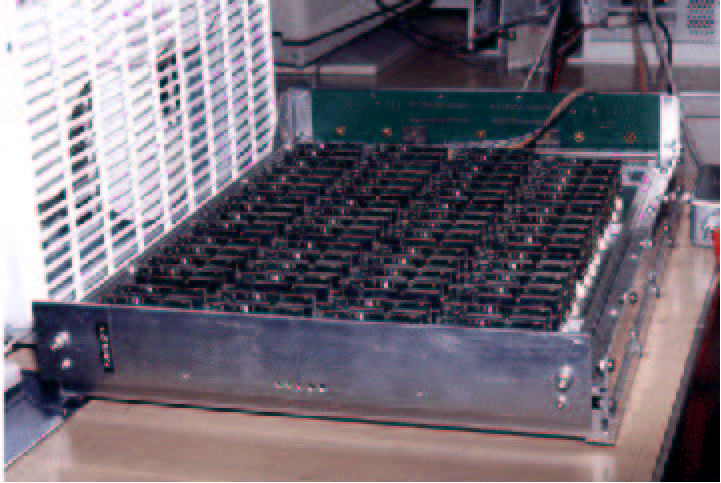
\includegraphics[width=4in]{motherboard_photo}
}
\end{center}
\caption{Photograph of a motherboard containing 63 daughterboard cards and
one integrated daughterboard. The motherboard is mounted on a test rig and 
is cooled by the fan on the left hand side}
\label{f:motherBoard}
\end{figure}

The daughterboards are connected on the motherboard in a four dimensional 
(4D) mesh via a {\em serial network} which is intended to be the main 
medium of communications for applications and hence it has been named
{\em the physics network}. The physics network is driven by the NGA 
of each daughterboard. This 4D serial network wraps around in each dimension,
giving each motherboard network topology of a {\em 4D--torus}.

All the daughterboards on a given motherboard are also connected to the 
special daughterboard 0 (the one integrated on the motherboard) via
a second serial network in a star topology. This network is part
of the so called {\em boot--diagnostic network}. The boot--diagnostic
network is used for hardware testing, and for downloading the various
boot and runtime kernels to the daughterboards at boot time. 

Each motherboard also has two SCSI ports which are connected to
daughterboard 0 on that board. These ports allow the connection of
daughterboards to either a front end host, to another motherboard, or
in future designs of the machine, to local disk systems. The SCSI
connections form part of the boot--diagnostic network and are not in
general expected to be heavily used in physics applications.

The motherboards are organised into crates. The {\em physics networks}
of the boards in a given cabinet are connected by a tagliatelle tangle
of flat ribbon serial cables into an overall physics network which
still forms a 4D torus.  The boot diagnostic networks of the boards in
a crate are connected via the SCSI interfaces on the motherboards into
a tree hierarchy. A picture of a crate is shown in figure \ref{f:crate}.
\begin{figure}[ht]
\begin{center}
\leavevmode
\hbox{%
\includegraphics{crate_photo}
}
\end{center}
\caption{A QCDSP crate holding 6 motherboards}
\label{f:crate}
\end{figure}

Finally the crates are assembled into a full machine.

In summary the communications in a machine are made up of two networks:
\begin{itemize}
\item
The Physics Network -- which is a serial network that to the programmers
point of view forms a 4D torus. This is the network that is intended for 
primary communications in an application.
\item
The Boot--Diagnostic network made up from a SCSI chain between motherboards,
rooted on the front end workstation. On each motherboard the boot--diagnostic
network is constructed from a serial network with a star topology rooted
on daughterboard 0.
\end{itemize}

A summary of the networks in QCDSP can be seen in figure \ref{f:networkSummary}.
\begin{figure}[ht]
\begin{center}
\leavevmode
\hbox{%
\includegraphics[width=4in]{networks_summary}
}
\end{center}
\caption{A summary diagram of QCDSP Networks showing three motherboards
connected in a tree of depth = 2. The horizontal and vertical
black lines show the physics network (2 dimensions of it) with the black
dots showing the daughterboards. The green lines show the SCSI tree and 
the red lines show the serial boot--diagnostic network. Purple lines 
show the connections between the SCSI ports and motherboard 0 on each 
board.}
\label{f:networkSummary}
\end{figure}

\section{Programming Interface}
The QCDSP at the simplest level provides a set of C++ functions
which may be called to achieve various aims. Broadly these functions
can be categorised as
\begin{itemize}
\item
Functions allowing the processor to identify itself and the machine
\item
Objects and functions for carrying out communications
\item
functions for self synchronisation
\item
miscellany -- random numbers etc .
\end{itemize}

\subsection{Header Files}
These functions are defined in the header file {\bf sysfunc.h} in the
directory {\tt /qcdsp/sfw/qos.<version>/usr/include} where {\tt
<version>} refers to the QOS revision as discussed in the previous
chapter. This directory should be listed as part of the {\tt TC\_DIR}
shell environment variable (see last chapter), thus making the
directory part of the default search path for the Tartan C++
compiler. The programmer merely needs to include the header file in
his source files using the directive
\begin{verbatim}
#include <sysfunc.h>
\end{verbatim} 
identically to the way he/she normally includes {\bf stdio.h}, {\bf stdlib.h}, 
{\bf math.h} and other standard header files.

\subsection{Unsupported C++ Features}
One should also be aware that not all of the standard ANSI C++ libraries
are implemented on the QCDSP. In particular the {\tt iostream} classes
are unavailable. The programmer needs to use the C standard I/O routines
defined in {\bf stdio.h}.

\subsection{Compilation and Running of Examples}
In the following sections we describe some of the functions provided 
in the {\bf sysfunc.h} file. To run the example codes we recommend that
the reader copies the {\em hello\_world} program as described in the last
section into his homedirectory and modifies the file {\bf main.C}. The makefile
provided can then be used to build the examples by typing the command {\tt make}. The resulting executable will be called {\bf hello\_world.out}. (Readers
with a knowledge of makefiles can adapt the makefile as they wish. The compiler
flags and command line options for the C++ compiler can be listed by typing
the command {\tt tcpp} with no arguments.) Let us
assume from here on that the {\em hello\_world} directory was copied to one
of identical name in the users homedirectory and that the results of all
compilations are named {\bf hello\_world.out}.

\section{Who Am I?}
\subsection{Knowing your identity and place in the Universe}
The following functions are defined in {\bf sysfunc.h} to enable
a processor to localise itself:
\begin{description}
\item{\tt int UniqueID()\ : \\}
This function returns an {\tt int} specifying 
the {\bf unique processor ID} of the calling
processor. (N.B: The MPI equivalent of this call
would be {\tt MPI\_Comm\_Rank}).
\item{\tt int NumNodes()\ : \\}
This function returns an {\tt int} specifying 
the total number of nodes
that are in use in the current machine partition.
(N.B: The MPI equivalent of this call would be {\tt MPI\_Comm\_Size}).
\item{\tt int MbNum()\ : \\}
This function returns an {\tt int} specifying the {\bf motherboard number}
of the motherboard on which the calling processor resides.
\item{\tt int DbNum()\ : \\}
This function returns an {\tt int} specifying the {\bf daughterboard number}
of the calling processor.
\item{{\tt int CoorT()}, {\tt int CoorX()}, {\tt int CoorY()}, {\tt int CoorZ()} \ : \\}
These function calls return {\tt int}-s specifying the T, X, Y and Z coordinates respectively, of the calling processor within the 4D torus of the physical
network.
\item{{\tt int SizeT()}, {\tt int SizeX()}, {\tt int SizeY()}, {\tt int SizeZ()} \ : \\} 
These functions return {\tt int}-s specifying the size of the 4D torus physical
network in the T, X, Y and Z directions respectively
\end{description}

Figure \ref{f:whoamiCode} shows a programming example, where the processors
in the QCDSP identify themselves and size up their machine parition using
these functions:
\begin{figure}[h]
\tiny
\begin{verbatim}
#include <stdio.h>
#include <stdlib.h>
#include <sysfunc,h>

int main(int argc, char *argv[])
{
   /* ------- What is my Unique ID  ---------------------- */
   int my_id = UniqueID();
   int num_processors = NumNodes();

   /* ------- Motherboard and Daughterboard Numbers -------*/
   int my_motherboard_num = MbNum();
   int my_daughterboard_num = DbNum();

   /* - My processor grid coordinates and grid dimensions -*/
   int my_coords[4];
   int proc_grid_dims[4];

   /* --------------- Get my coordinates ----------------- */
   my_coords[0] = CoorT();
   my_coords[1] = CoorX();
   my_coords[2] = CoorY();
   my_coords[3] = CoorZ();

   /* - Get information about the processor grid size ---  */
   proc_grid_dims[0] = SizeT();
   proc_grid_dims[1] = SizeX();
   proc_grid_dims[2] = SizeY();
   proc_grid_dims[3] = SizeZ();

   /* -  Echo Back information to the user --------------- */
   printf("I am processor: %d.\n", my_id);
   printf("I live on motherboard %d, daughterboard %d\n",  my_motherboard_num,
                                                             my_daughterboard_num);

   printf("I am one of a total of %d computing elements\n", num_processors);
  
   printf("The current physical network has the following dimensions\n");
   printf("%d Processors in the T direction\n", proc_grid_dims[0]);
   printf("%d Processors in the X direction\n", proc_grid_dims[1]);
   printf("%d Processors in the Y direction\n", proc_grid_dims[2]);
   printf("%d Processorz in the Z direction\n", proc_grid_dims[3]);
  
   printf("My (T,X,Y,Z) coordinates are (%d, %d, %d, %d )\n", 
           my_coords[0], my_coords[1], my_coords[2], my_coords[3]);

   return(EXIT_SUCCESS);
}
\end{verbatim}
\caption{Sample program showing use of self identification functions.}
\label{f:whoamiCode}
\end{figure}   

Running the code in figure \ref{f:whoamiCode} on the 64 daughterboard 
development board {\em q\_2} produced the following results:
{
\scriptsize
\begin{verbatim}
(qcdhost/homeqs0/bj/hello_world: qcsh[q_2])% qrun hello_world.out
.
.
.
I am processor: 0.
I live on motherboard 0, daughterboard 0
I am one of a total of 64 computing elements
The current physical network has the following dimensions
4 Processors in the T direction
4 Processors in the X direction
2 Processors in the Y direction
2 Processorz in the Z direction
My (T,X,Y,Z) coordinates are (0, 0, 0, 0 )
.
.
.
\end{verbatim}
}

Using the command {\tt qprintf} command as described in the last chapter
allows one to look at the output buffers of some of the other processors:
{\scriptsize
\begin{verbatim}
.
.
.
Qdaemon:  user print buffer for Mb 0 and Db 2 (SCSI tree coordinates)
Buffer wrap count 0
I am processor: 2.
I live on motherboard 0, daughterboard 2
I am one of a total of 64 computing elements
The current physical network has the following dimensions
4 Processors in the T direction
4 Processors in the X direction
2 Processors in the Y direction
2 Processorz in the Z direction
My (T,X,Y,Z) coordinates are (0, 0, 1, 0 )
.
.
.
Qdaemon:  user print buffer for Mb 0 and Db 63 (SCSI tree coordinates)
Buffer wrap count 0
I am processor: 63.
I live on motherboard 0, daughterboard 63
I am one of a total of 64 computing elements
The current physical network has the following dimensions
4 Processors in the T direction
4 Processors in the X direction
2 Processors in the Y direction
2 Processorz in the Z direction
My (T,X,Y,Z) coordinates are (3, 3, 1, 1 )
\end{verbatim}
}

\subsection{Some useful enumerated types}
You may notice\footnote{if you haven't yet please do so now}
if you look through the code in \ref{f:whoamiCode} that
I have always ordered the indices of both the {\tt my\_coords} and {\tt proc\_grid\_dims} in the order T, X, Y and Z with the T corresponding to the index
0 and Z corresponding to index 3. To make for much more
readable programs there exists an enumerated type called {\tt SCUAxis}.
A variable of type {\tt SCUAxis} can take on only four values
\begin{description}
\item{\tt SCU\_T -- \ } 
for the T direction,
\item{\tt SCU\_X -- \ } 
for the X direction,
\item{\tt SCU\_Y -- \ } 
for the Y direction and 
\item{\tt SCU\_Z -- \ } 
for the Z direction \ .
\end{description}
The actual definition of the type:
{\scriptsize \begin{verbatim}
enum SCUAxis { SCU_T, SCU_X, SCU_Y, SCU_Z };
\end{verbatim}}
ensures that the integer values of the enumerations
are {\tt SCU\_T}=0, {\tt SCU\_X}=1, {\tt SCU\_Y}=2 and {\tt SCU\_Z}=3
respectively. 

Thus we should be able to index our arrays with these enumerations
rather than with the integers 0,1,2 and 3 as before. For example
we could write
{\scriptsize \begin{verbatim}
my_coords[SCU_X]=CoorX(); /* equivalent to my_coords[1] = CoorX() */
\end{verbatim}} 
or for example we could cycle through all the directions in the 
processor grid with the following {\tt for} loop:
{\scriptsize \begin{verbatim}
int i;
for(i = SCU_T; i <= SCU_Z; i++) {
  /* do something exciting here  */
}
\end{verbatim}}

Incidentally, we note that this latter use relies on the particular
ordering of the axes defined in the enumerated type. In future releases
of QOS, the ordering of the enumerated elements maybe different from 
the current release. If this happens the above for loop may not be 
portable. Hence, {\em caveat emptor}. The enumerated type itself 
is defined in {\tt /qcdsp/sfw/qos.<version>/include/scu\_enum.h} which
is included in the {\bf sysfunc.h} file. ({\em Suggestion:
perhaps a member of the enumerated type called MAX\_AXIS or something
should be defined for such loops. They could then be written as
} {\tt for(i=0; i< MAX\_AXIS; i++) })

\section{Nearest Neighbour Communications}
The QCDSP {\bf sysfunc.h} header files defines several ways of carrying
out nearest neighbour communications. We will look into the simplest one
here. By communication we mean sending/receiving a certain number of bytes
from one processor to another. On the QCDSP such a communication is made up of
three stages.
\begin{description}
\item{\bf Preparation: \ } -- the sender/receiver describes the data
to be sent/received and provides a pointer in memory to the data that
is to be sent / to where the data is to be received
\item{\bf Initiation: \ } --  the sender / receiver initiates the 
communication. The sender / receiver is then free to carry out other
tasks.
\item{\bf Completion: \ } -- the sender / receiver wait until the 
communication is complete, in the case of the sender this means that 
all the data has been sent and in the case of the receiver it means that
the the data has arrived.
\end{description}
Communication along the physical network is handled by the Serial
Communication Unit (SCU) in the NGA chip, and the communication does
not need much interaction from the CPU past the initiation
stage. Hence the time spent communicating allows the processor to
carry out computation while the communication proceeds. It is only
immediately before using the results of the communications that the
processor has to wait to make sure that the communication is
complete. (Note: This is similar in style to the MPI non--blocking
communications, however in the case of MPI the so called preparation
and initiation stages are usually rolled into one)

\subsection{Preparation}
In preparing to communicate we must decide upon the following things:
\begin{itemize}
\item
Who did we want to communicate with? This is generally one of our
neighbours. We have neighbours in eight directions, these being 
the positive and negative T, X, Y and Z directions respectively. An enumerated type, {\tt SCUDir}, is made available to help us in writing safe, 
maintainable programs. This enumerated type is made accessible through
the header file {\bf sysfunc.h}. The actual enumerations are
\begin{description}
\item{ {\tt SCU\_TM} (T, Minus): \ } 
-- Communicate in the negative T direction
\item{ {\tt SCU\_TP} (T, Plus): \ } 
-- Communicate in the positive T direction
\item{ {\tt SCU\_XM} (X, Minus): \ }
-- Communicate in the negative X direction
\item{ {\tt SCU\_XP} (X, Plus) : \ }
-- Communicate in the positive X direction
\item{ {\tt SCU\_YM} (Y, Minus): \ } 
-- Communicate in the negative Y direction
\item{ {\tt SCU\_YP} (Y, Plus): \ } 
-- Communicate in the positive Y direction
\item{ {\tt SCU\_ZM} (Z, Minus): \ }
-- Communicate in the negative Z direction
\item{ {\tt SCU\_ZP} (Z, Plus) : \ }
-- Communicate in the positive Z direction
\end{description}
\item 
We must decide whether we wish to send a message or receive one.
Once again we have an enumerated type at our disposal called
{\tt SCUXR}. This can have only two values:
\begin{description}
\item{ {\tt SCU\_REC} : \ } 
receive operation
\item{ {\tt SCU\_SEND} : \ } 
send operation.
\end{description}
\item
We must describe our data. For our purposes the data shall consist 
of a number of blocks, each block having a certain length. The blocks
need not be contiguous in memory, but may have some regular spacing
between them. The distance in memory ({\bf in units of blocks}) separating
the {\bf start of one block} from the {\bf start of the next one} is called
the data stride.

Hence our messages are completely described by specifying the {\em
memory address} of the first block, {\em the length of a block in
bytes}, {\em the number of blocks in the message} and {\em the
stride}.  For messages made up of a contiguous set of blocks, the
stride is always one. In other words, the start of a block in memory is
always one block-length away from the start of the previous block with the
intervening memory between the two being filled up by the body of
the first block. The idea of this data description scheme is illustrated
in figure \ref{f:message}.
\end{itemize}

\begin{figure}[h]
\begin{center}
\leavevmode
\hbox{
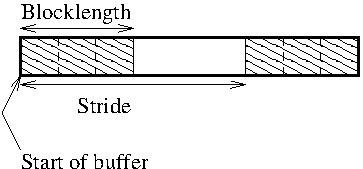
\includegraphics{message}}
\end{center}
\caption{Anatomy of a message. Here the message consists of 2 blocks
(shaded) with each block having a block length of 3 bytes. The blocks
are not contiguous but have a block separation between them making the
stride value for this message 2}
\label{f:message}
\end{figure}

On the QCDSP the preparing to communicate involves the instantiation
of a so called {\tt SCUDirArg} object. There are several ways of
carrying out this instantiation. Perhaps the simplest is to use the
{\em constructor}: 
{\small \begin{verbatim} 
SCUDirArg(void *buffer, SCUDir dir, SCUXR xr, int blklen, 
          int numblk = 1, int stride = 1).
\end{verbatim}}
This method allows the complete description of the putative communication to be specified with one single statement. The arguments have the following meaning:
\begin{description}
\item{\tt void *buffer \ } 
this is a pointer to the start of the message in memory. It is of type {\tt void *} so that the pointer can point to data of any type. 
\item{\tt SCUDir dir \ } 
this is the direction in which the communication is to proceed and should take
the value of one of the 8 enumerations of the enumerated type {\tt SCUDir } listed above.
\item{\tt SCUXR xr \ } 
indicates whether we are sending or receiving. This should take one of the two 
values of the enumerated type {\tt SCUXR} listed above.
\item{\tt int blklen \ } 
gives the length in bytes of a single block to be transmitted/received.
\item{\tt int numblk = 1 \ }
gives the number of blocks to be communicated. This is an optional
argument to the constructor, which, if unspecified will have the
default value of 1, indicating that there is only a single block to be
communicated
\item{\tt int stride = 1 \ }
specifies the stride of the data. This is an optional argument to the constructor, which, if unspecified will have the default value of 1 corresponding to the 
contiguous data.
\end{description}

As an example, suppose I wanted to send an integer in the 
positive X direction, I could instantiate the communication description object as:
\begin{verbatim}
int number_to_send = 5;
SCUDirArg send_int_x_plus((void *)&number_to_send, SCU_XP, 
                          SCU_SEND, sizeof(int));
\end{verbatim}
or as:
\begin{verbatim}
int number_to_send = 5;
SCUDirArg send_int_x_plus((void *)&number_to_send, SCU_XP, 
                                  SCU_SEND, sizeof(int),1);
\end{verbatim}
or even as:
\begin{verbatim}
int number_to_send = 5;
SCUDirArg send_int_x_plus((void *)&number_to_send, SCU_XP, 
                                  SCU_SEND, sizeof(int),1,1);
\end{verbatim}
where in the last two cases I have explicitly specified the optional arguments.
In all the above cases the result of the instantiation is an
object of type {\tt SCUDirArg} with name {\tt send\_int\_x\_plus}. This object
now acts as a {\em handle} to that particular communication.

Likewise to receive a 5-vector of floating point numbers of type {\tt float}
from the negative Y direction, I would set up the communication as:
\begin{verbatim}
float receive_buffer[5];
SCUDirArg rec_floats_y_minus((void *)receive_buffer, SCU_YM, 
                             SCU_REC, sizeof(float), 5, 1);
\end{verbatim}

Alternatively, I can set up the communication to send the 5 members of a 10 member integer array which have odd indices in the positive T direction using the
following instantiation:
\begin{verbatim}
int send_buffer[10];
SCUDirArg send_odd_t_plus((void *)&send_buffer[1], SCU_TP, 
                          SCU_SEND, sizeof(int), 5, 2);
\end{verbatim}

The {\tt SCUDirArg} objects can also be instantiated and manipulated using
various other {\em class methods}. For example I can instantiate an
object, without a description of the communication to be performed 
by simply using the default constructor:
\begin{verbatim}
SCUDirArg for_later;
\end{verbatim}
Later on I can initialise this object with the method {\tt Init}
which has the same argument list as the full constructor described earlier.
Hence I can either set up the object in the previous manner as:
\begin{verbatim}
int number_to_send = 5;
SCUDirArg send_int_x_plus((void *)&number_to_send, SCU_XP, 
                          SCU_SEND, sizeof(int));
\end{verbatim}
or alternatively I can use the {\tt Init} method:
\begin{verbatim}
int number_to_send = 5;
SCUDirArg send_int_x_plus;
send_int_x_plus.Init((void *)&number_to_send, SCU_XP, 
                          SCU_SEND, sizeof(int));
\end{verbatim}

Other methods by which the data description elements of the object can be
set are
\begin{description}
\item{\tt void * Addr( void *addr) \ }
the start of the data is set to {\tt addr}. The address of the new
buffer is returned.
\item{\tt int Blklen( int blklen ) \ }
the block length of the communication is set to {\tt blklen}. The 
new block length is returned.
\item{\tt int Numblk( int numblk ) \ }
the number of blocks in the transfer is set to {\tt numblk}. The new
number of blocks is returned.
\item{\tt int Stride( int stride ) \ } 
the stride of the transfer is set to {\tt stride}. The new stride is returned.
\item{\tt void Reload(void *a, int blklen, int numblk=1, int stride = 1) \ }
The new data description indicated in the argument list is set (the send/receive nature of the data or the communication direction remain as before). {\tt a} holds the address of the start of the data. The remaining arguments should be
self explanatory by now. Note again that the last two arguments are optional.
\end{description}

So for example to send first an {\tt int}, then a {\tt float} in the 
positive X direction followed by a second {\tt int} communication, I can 
instantiate the communication object for the first {\tt int}  and then simply
use the methods above to change the data description:
\begin{verbatim}
int int_buf=5;
int float_buf=0.6;

/* Set up the integer communications */

SCUDirArg send_x_plus((void *)&int_buf, SCU_XP, 
                      SCU_SEND, sizeof(int));

/* 
 * Carry out the first communications here 
 */

/* Now change to float communications -- send in the same direction */
send_x_plus.Addr((void *)&float_buf);
send_x_plus.Blklen(sizeof(float));
 
/* 
 * Carry out the second communication here
 */

/* Now prepare to send  an int again -- last two arguments optional */
send_x_plus.Reload((void *)&int_buf, sizeof(int));

/*
 * Carry out the third communication here
 */
\end{verbatim}

\subsection{Initiating the Communications}
Once we have defined the type of communication we wish to perform,
we must initiate the data transfer. This is done by the function
{\tt SCUTrans}. There are several ways of using {\tt SCUTrans}, here I will
describe the simplest one.

Calling {\tt SCUTrans} with the address of an {\tt SCUDirArg} object as the 
sole argument will initiate the communication encoded in that object.

As an example, suppose we want to send the integer 4 in the positive X
direction and an {\tt SCUDirArg} object {\tt int\_x\_plus} has been
instantiated to describe this communication ({\em Exercise:
Instantiate an SCUDirArg object to encode this communication.}) The
communication could then be initiated by the following call:
\begin{verbatim}
SCUTrans( &int_x_plus );
\end{verbatim}
However the results of the communication will not be available until the
communication completes.

\subsection{Completing the Communication}
To complete the communication the program should call the function
{\tt SCUTransComplete}. One can call this function with the address
of an {\tt SCUDirArg} object to complete to communication encoded in 
that, or without any arguments to complete all outstanding communications.
There is also another way to call {\tt SCUTransComplete} to match a 
particular way of calling {\tt SCUTrans} which will not be detailed here.

Hence to complete the previously initiated transfer encoded in the object
{\tt x\_int\_plus} of the last subsection, one should call
\begin{verbatim}
SCUTransComplete( &x_int_plus);
\end{verbatim}

To complete all outstanding communications on a given processor ({\bf
this does not imply a synchronisation across processors}) one should
instead call 
\begin{verbatim}
SCUTransComplete();
\end{verbatim}

\section{Getting To Know Your Neighbours}
Before concluding this chapter, we present the code for a complete program
designed to show the use of some of the communication routines presented
in the last section. 

The program discovers the processor ID's of its neighbours in every direction.
For each axis, T, X, Y and Z, the processors send their unique ID's in the
positive direction, and receive the ID's of their neighbours from the negative
direction.

Once this is done for all four axes, the communication pattern is
repeated but in the opposite direction. That is, for all four axes,
each processor will send its unique ID in the negative direction and
receives the ID of its neighbour from the positive direction.  When
this process is done for all the axes, the processor will have the ID's of
all its neighbours.

{\scriptsize
\begin{verbatim}
#include <stdio.h>
#include <stdlib.h>
#include <sysfunc.h>

// --------------------------------------------------------------------
// This function, when given the direction to send in (send direction)
// will send the contents of its send_buffer in that direction and 
// will receive into its receive buffer from the negative direction
// -------------------------------------------------------------------
void neighbourSend(int *send_buffer, int *recv_buffer,
                   SCUDir send_direction)
{

   SCUDir recv_direction;

   // ------------------------------------------------------------- //
   // Figure out the receive direction                              //
   // ------------------------------------------------------------- //

   switch( send_direction ) {

        case SCU_TM : recv_direction = SCU_TP;
                        break;

        case SCU_TP : recv_direction = SCU_TM;
                        break;

        case SCU_XM : recv_direction = SCU_XP;

                      break;

        case SCU_XP : recv_direction = SCU_XM;
                      break;

        case SCU_YM : recv_direction = SCU_YP;
                      break;

        case SCU_YP : recv_direction = SCU_YM;
                      break;

        case SCU_ZM : recv_direction = SCU_ZP;
        break;

        case SCU_ZP : recv_direction = SCU_ZM;
        break;

        default: fprintf(stderr, "P%d: Error Invalid Send Direction\n");
                         exit(EXIT_FAILURE);
                         break;
   }
   // ------------------------------------------------------------- //
   // Set up SCUDirArg objects, one for send and one for receive    //
   // ------------------------------------------------------------- //

   // ------------------------------------------------------------- //
   // Send an integer in the send direction                         //
   // ------------------------------------------------------------- //
   SCUDirArg send( send_buffer,
                   send_direction,
                   SCU_SEND,
                   sizeof(int));

   // ------------------------------------------------------------- //
   // Recieve an integer from the opposite direction                //
   // ------------------------------------------------------------- //
   SCUDirArg recv( recv_buffer,
                   recv_direction,
                   SCU_REC,
                   sizeof(int));

   // ------------------------------------------------------------- //
   // Initiate the transfer                                         //
   // ------------------------------------------------------------- //

   SCUTrans( &send );
   SCUTrans( &recv );

   // ------------------------------------------------------------- //
   // Wait for these two specific transfers to complete             //
   // ------------------------------------------------------------- //

   SCUTransComplete( &send );
   SCUTransComplete( &recv );

   // ------------------------------------------------------------- //
   // Done                                                          //
   // ------------------------------------------------------------- //
}

int main(int argc, char *argv[])
{
   // ------------------------------------------------------------ //
   // Details about myself                                         //
   // ------------------------------------------------------------ //

   int my_id=UniqueID();
   int my_coords[4] = { CoorT(), CoorX(), CoorY(), CoorZ() };

   // ------------------------------------------------------------ //
   // Print out information about the grid                         //
   // ------------------------------------------------------------ //

   printf("Processor grid has dimensions: T=%d X=%d Y=%d Z=%d\n",
          SizeT(),
          SizeX(),
          SizeY(),
          SizeZ());

   // ------------------------------------------------------------ //
   // Print out information about ourselves                        //
   // ------------------------------------------------------------ //


   printf("P%d, T=%d, X=%d, Y=%d, Z=%d\n",
          my_id,
          my_coords[SCU_T],
          my_coords[SCU_X],
          my_coords[SCU_Y],
          my_coords[SCU_Z]);

   // ------------------------------------------------------------ //
   // Now Send my ID to my neighbour in each dimension             //
   // ------------------------------------------------------------ //

   int neighbour_id[8];         // -- Array to hold information about
                                //    neighbours

   SCUDir counter;              // A direction counter variable

   // ----------------------------------------------------------- //
   // This next bit is a little naughty as it relies on the fact  //
   // Ordering of the members of the enumerated types             //
   // ----------------------------------------------------------- //
   // Transmit my ID in  the positive directions                  //
   // and receive ID from the negative direction                  //
   //                                                             //
   // Note that Axis_plus = Axis_minus + 1 in the enumeration     //
   // hence the choices of the counter                            //
   // ----------------------------------------------------------- //
    
   // -----------------------------------------------------------------
   // First send our ID-s to the +ve  directions (receive from -ve)
   // -----------------------------------------------------------------

   for(counter = SCU_TM; counter <= SCU_ZM; counter+=2) {
     neighbourSend( &my_id,
                    &neighbour_id[ counter ],
                    counter + 1 );
                    
   }
 
   // ------------------------------------------------------------------
   // Second send our ID-s to the -ve directions (receive from +ve)
   // ------------------------------------------------------------------
  
   for(counter = SCU_TP; counter <= SCU_ZP; counter+=2) {
     neighbourSend( &my_id,
                    &neighbour_id[ counter ],
                    counter - 1 );
   }

   // ---------------------------------------------------------- //
   // Print out my neighbours IDs                                //
   // -----------------------------------------------------------//

   printf("P%d:  T-Neighbour (-,+): (%d, %d)\n",
          my_id,
          neighbour_id[ SCU_TM ],
          neighbour_id[ SCU_TP ] );


   printf("P%d:  X-Neighbour (-,+): (%d, %d)\n",
          my_id,
          neighbour_id[ SCU_XM ],
          neighbour_id[ SCU_XP ] );

   printf("P%d:  Y-Neighbour (-,+): (%d, %d)\n",
          my_id,
          neighbour_id[ SCU_YM ],
          neighbour_id[ SCU_YP ] );

   printf("P%d:  Z-Neighbour (-,+): (%d, %d)\n",
          my_id,
          neighbour_id[ SCU_ZM ],
          neighbour_id[ SCU_ZP ] );

}
\end{verbatim}
}

\section{Summary of Chapter}
In this chapter we have outlined some of the basic system
calls provided by the QCDSP {\bf sysfunc.h} and how they
can be used for processors to identify themselves and to 
perform simple nearest neighbour communications.

\subsection{Architecture summary}
The main point to stress about the computer architecture is that
there are two main networks in the QCDSP. One is the boot--diagnostic
network and the other is the physics network. The boot--diagnostic 
network is partly made up of a SCSI tree structure, partly of a 
serial network with a star topology rooted on the special embedded
daughterboard on each motherboard. The physics network is a 4-D
torus.

\subsection{Self Identification Summary}
Several routines are provided in the header file {\bf sysfunc.h}.
These include the functions 
\begin{description}
\item{\tt int UniqueID() \ } -- returns the processor ID
\item{\tt int NumNodes() \ } -- returns the number of processors
\item{\tt int MbNum()    \ } -- returns the processors motherboard number
\item{\tt int DbNum()    \ } -- returns the processors daughterboard number
\item{\tt int CoorT(), int CoorX(), int CoorY(), int CoorZ() \ } -- returns
the processors coordinates in the physical network.
\item{\tt int SizeT(), int SizeX(), int SizeY(), int SizeZ() \ } -- returns
the sizes of the physical network in the respective dimensions.
\end{description}

\subsection{Enumerated Types Summary}
The following enumerated types are defined in the hearder file {\bf sysfunc.h}
\begin{description}
\item{\footnotesize \tt enum SCUAxis = \{ SCU\_T, SCU\_X, SCU\_Y, SCU\_Z \}; \ } -- a type to describe the four axes of the physical network
\item{\footnotesize \tt enum SCUDir = \{ SCU\_TM, SCU\_TP, SCU\_XM, SCU\_XP, SCU\_YM, SCU\_YP, SCU\_ZM, SCU\_ZP \}; \ } -- a type to enumerate the 8 communication
channels available on each processor. The naming convention is {\tt
SCU\_<Axis><P/M>} where {\tt <Axis>} is one of T, X, Y or Z and {\tt
<P/M>} is either P for the positive (plus) direction along the axis or
M for the negative (minus) direction along the axis
\item{\footnotesize \tt enum SCUXR = \{ SCU\_REC, SCU\_SEND= 8\}; \ } -- enumerates
the two types of communications, sending or receiving. Note that {\tt
SCU\_SEND} has an integer value of 8 rather than 1.
\end{description}

\subsection{Nearest Neighbour Communications Summary}
Nearest neighbour communications can be initiated by the {\tt SCUTrans}
function and completed by the {\tt SCUTransComplete} function. The description
is specified via an {\tt SCUDirArg} object.

The {\tt SCUDirArg} objects can be instantiated through invoking the 
constructor
\begin{verbatim}
SCUDirArg(void *buffer, SCUDir dir, SCUXR xr, int blklen, 
          int numblk = 1, int stride = 1);
\end{verbatim} 
where the arguments respectively are the address of the start of the
data, the direction of the communication, the mode of communication
(SEND/RECEIVE), the blocklength of the data to be communicated (in
bytes), the number of blocks to communicate and the data stride. The
last two of these parameters are optional. The default number of blocks
is 1 indicating a single item transfer. The default stride is 1 indicating
contiguous blocks.

Other forms of the {\tt SCUDirArg} constructor are also available.
(See more advanced documentation if I ever write it).

The {\tt SCUTrans} function call has a prototype
\begin{verbatim}
void SCUTrans( SCUArgDir *arg );
\end{verbatim}
where {\tt arg} is a pointer to the {\tt SCUArgDir } object describing
the communication. A call to {\tt SCUTrans } initiates a communication.
The communication should not be considered complete until a corresponding
{\tt SCUTransComplete} call returns. The {\tt SCUTrans } function has
other (overloaded) prototypes which were not discussed here. (See more
advanced documentation if I ever write it).

The {\tt SCUTransComplete} function call has prototypes
\begin{verbatim}
void SCUTransComplete( SCUArgDir *arg );
void SCUTransComplete();
\end{verbatim}
The first of these takes as its argument a pointer to an {\tt SCUArgDir} object.
In this case the function returns when the communication encoded in the
object pointed to by {\tt arg} completes. In the second case the function
has no arguments. In this case the function returns when all the 
communications currently pending complete.

In the next chapter we shall discuss simple global communication algorithms
and their implementation using the functions detailed in this chapter.

\section{Programming Exercise}
\subsection{The Problem: -- More efficient Neighbours}
The program for discovering our neighbours can be made more efficient. Currently, a node only performs two communications at a time in each direction; one send and one receive. In principle, a processor could send its ID along all 8
available direction. Likewise, its neighbour could receive along all 8 of its
communication channels. The goal of this exercise is for you to write a
program that discovers its neighbours in this manner.

\subsection{Checkerboard Partitioning}
Checkerboard partitioning of processors (also known as even--odd partitioning
or red--black partitioning) assigns a parity (colour) to each processor which
can be either even (red) or odd (black). The name checkerboard partitioning
comes from the fact neighbouring processors have opposite parities (colours).
See figure \ref{f:checkerboard_proc} for a picture of a two dimensional 
processor grid separated into even and odd (red and black) sites.
\begin{figure}[h]
\begin{center}
\leavevmode
\hbox{%
\includegraphics{checkerboard_proc}
}
\end{center}
\caption{A 4x4 grid of processors with checkerboard partitioning. Note that
any one processor has oppositely coloured neighbours}
\label{f:checkerboard_proc}
\end{figure}

The idea here that in the end processors of one colour (say red) can
send their ID's to all their neighbours of the other colour (in this
case black), while processors of the other colour (black) can receive
along all 8 of their wires. Hence half of all the processors (the
black ones) can discover the identities of all their neighbour in one
single communication step. The communication could then be repeated, with
the colours interchanged. In other words, in the second communication,
all the processors of the second colour (black in this case) can transmit
their IDs to processors of the first colour (red).

Thus all the nearest neighbours can be discovered using in effect two
communication steps.

\subsection{Exercise 1: Am I red or am I black} 
Let the two parities be denoted 0 (for red say) and 1 (for black). First
thing the processor has to do is identify its parity. It could do this 
for example based on its coordinates in the physics network. Implement
a routine using the relevant system calls by which each processor determines
its parity.

\subsection{Exercise 2: Do the transfer}
Implement the neighbour discovery algorithm outlined above.

\chapter{Collective Communication}
\section{What are Collective Communications ?}
In the previous chapter we have briefly described the basic {\tt SCU} 
calls for nearest neighbour point to point communication. This 
kind of communication is fine if we want to program communications
between processors that are reminiscent of the HPC {\tt CSHIFT} 
function for example, or if we wish to build systolic array like 
systems.

Occasionally however we may want to perform certain global communications
such as a sum of data items held across all the processors. An immediate
example of such a situation is the case of taking the scalar product of two vectors. Imagine that the vector
components are distributed amongst the nodes of the parallel computer. Each 
processor could work out the sum of the squares of its local vector components
but to accumulate the dot product, these local results would have to be
globally summed. 

\section{Who Communicates?}
The distinguishing feature of global communications also known
sometimes as collective communications is that all the processors make
the call to the communication routines, whereas in the case of a point
to point communication, usually only the sending and the receiving
node call a communication routine.

In the case of MPI and other message passing standards usually one has
a way of selecting subgroups of processor nodes from a given available
set. In MPI for example the so called 'communicator' {\tt
MPI\_COMM\_WORLD} refers to all available processors and subgroups of
these can be identified by defining new communicators (using such
routines as {\tt MPI\_Comm\_split}.)

In the case of the QCDSP, selecting processor partitions is non
trivial. Machines are often 'manually hardware partitioned' ( a
technical process involving graduate student plugging wires on the
backplanes of crates ).  Alternatively, in a given hardware partition,
one may select a certain set of processors using the QOS command {\tt
qset\_nodes }.  Once a given set of nodes is selected by either method
however, it is non--trivial to sub--select again from within a running
program.  Consequentially, our description of collective
communications will refer to situations when all available processor
nodes take part in the communication. These kinds of collective
communications are referred to as global communications. From here on
we shall use the two phrases interchangeably.

\section{Global Communication in General}
We now describe some common types of collective communication.
Since a lot of these are in the MPI message passing interface
specification I shall refer frequently to MPI equivalents. If
you know MPI this should make things easy for you. It should
also clear up ambiguities (I hope) in other situations.

\subsection{Barrier} 
A {\em barrier} routine is used to synchronise a set of processors.
All the nodes call the barrier routine. The routine does not exit
until all the processes participating in the communication have
entered it. In MPI one would require a call to the function {\tt
MPI\_Barrier}. In the case of the QCDSP the functionality is provided
through the system call {\tt sync()}, which is defined in the system
header file {\tt sysfunc.h}.

\subsection{Broadcast}
There are two general kinds of broadcast routines. They are 
\begin{description}
\item{\bf One To All Broadcast: \ }
This is procedure where a given processor node (usually referred to as
the root processor) contains some information. This information 
is sent to all other processors during a one to all broadcast routine.
\item{\bf All to All Broadcast: \ }
This is a procedure where at the outset each processor has an item
of data, and during the broadcast procedure each processor makes available
its data to all other processors. At the end of the broadcast, all
the processors are in possession of the data elements from all the other
processors.
\end{description}

The idea of the two kinds of broadcasts are illustrated in figures
\ref{f:oneToAllBroadcast} and \ref{f:allToAllBroadcast} respectively.
\begin{figure}[h]
\begin{center}
\leavevmode
\hbox{%
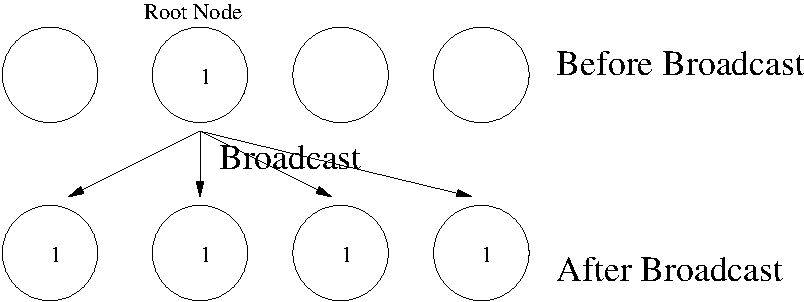
\includegraphics{one_to_all_bcast}
}
\end{center}
\caption{One to all broadcast. The circles represent
processor nodes. Before the broadcast, the root node holds the data
item to be distributed, in this case the number 1. After the
broadcast, the data item is found on all processors}
\label{f:oneToAllBroadcast}
\end{figure}

\begin{figure}[h]
\begin{center}
\leavevmode
\hbox{%
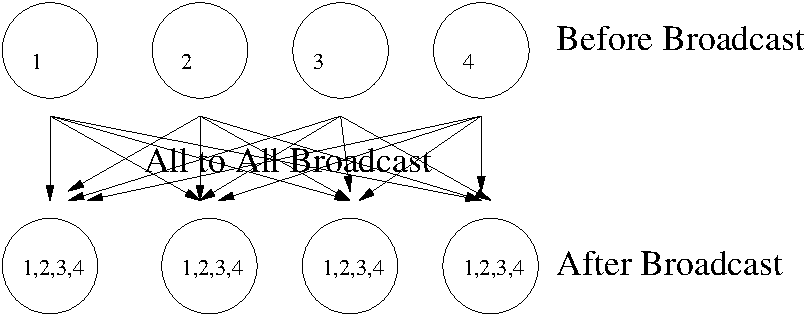
\includegraphics{all_to_all_bcast}
}
\end{center}
\caption{All to all broadcast: The circles represent processor nodes.
Before the broadcast all items hold their own data (the numbers inside 
them). After the broadcast, each processor has a copy of everybody 
else's data.}
\label{f:allToAllBroadcast}
\end{figure}

Important uses of broadcast operations can include the distribution
of parameters from a source processor as well as situations where 
one processor has to be a 'master' and has to make global decisions.
These decisions then probably need to be broadcast out to the other processors.

\subsection{Gather and Scatter}
The {\em gather} operation is one in which all processors send their
data to a nominated root processor. Its opposite is the so called 
{\em scatter operation} where the nominated root processor distributes
a vector of data, to the whole processor grid. The operations are illustrated
in figure \ref{f:gatherscatter}.
\begin{figure}
\begin{center}
\leavevmode
\hbox{%
\includegraphics{gatherscatter}
}
\end{center}
\caption{Above: Scatter operation. One processor 'scatters' its data
amongst the complete set. Below: Gather operation: The data from all
processors is 'gathered' onto a root processor.}
\label{f:gatherscatter}
\end{figure}
Sometimes the terms {\em gather} and {\em scatter} are generalised, to
mean that one processor distributes its data to some subset of other
processors (for example its nearest neighbours in the processor
grid). In this sense the corresponding gather would be the collection
of data from the same subset of processors.

In fact the broadcast operation can be implemented as a scattering
operation, where all processors receive the same data item. Likewise
the neighbour discovery exercise at the end of the last exercise (have
you attempted it?)  is an example where we combine a generalised
gather and a generalised scatter.  The generalised gather is that each
node (of a given parity) receives the processor ID of its nearest
neighbours, whereas the generalised scatter is the part where every
node (of the opposite parity) sends its ID to its nearest
neighbours. The MILC collaboration, in their code\footnote{Freely available at {\tt  http://cliodhna.cop.uop.edu/\~hetrick/milc/}. You could do us a great
service if you ported it to the QCDSP...} has refined the
generalisation of gathering and scattering to such a level where a
user can actually define his or her own gather and scatter mapping.

Scatter and Gather operations are useful for example to distribute data
that has just been read from disk by a master processor (assuming of course
that the master processor can hold all the data in memory) or to pass out
processor specific decisions. It can also be used, as mentioned before
to implement the broadcast operation. Generalised scatters can be useful
for exchanging data boundaries between processors for example.

\subsection{Global Reduction}
Global reduction operations generally take data from each node and
produce one single (reduced) result. Examples of global reduction are
global sums, global products, global XOR operations, finding global
minima and maxima. In fact any associative operation can be used as a
reducing operation. It perhaps for this reason that MPI has only two
functions {\tt MPI\_Reduce} and {\tt MPI\_Allreduce} to carry out all
their reduction operations\footnote{The actual operation and type of
data are specified using tags such as {\tt MPI\_INT} and {\tt MPI\_SUM}
for example}, instead of having separate global sum, global XOR and
other global routines.
 
Once again there are two kinds of global reduction operations.
\begin{description}
\item{\bf All to One Reduction: \ } -- these are reduction operations
where the final answer is left with one nominated (root) processor. 
These correspond to {\tt MPI\_Reduce}.
\item{\bf All to All Reduction: \ } -- these are reduction operations
where the final answer is given to every processor. These correspond 
to {\tt MPI\_Allreduce}. 
\end{description}

It should be clear for example that one can implement all to all 
reduction operations as an all to one reduction operation followed 
by a broadcast.

An important use of global sums for example is in the computation
of scalar products. A use of a global maximum operation for example
would be to find the infinity norm of a distributed vector. Global
XOR operations may be needed for checksumming a distributed dataset.
A quick and dirty floating point broadcast routine could be written
using a global sum where the root node contributes to the sum the 
amount it wishes to broadcast and all the other processors contribute
0. 

A {\bf warning} about global sums and other global operations which
are susceptible to cancellation errors and or bit overflow problems:
The QCDSP system can contain anything from between 64 nodes to
O($10^5$) nodes. Even if a single node has only component to contribute
to a particular reduction, it is possible that when for example 16K 
processors are involved in an operation there is a serious chance
of overflow or that cancellation errors have a serious effect.
There are two ways to address this problem:
\begin{itemize}
\item
The implementors should implement their reduction operations in 
such a way as to minimise the problems of rounding error accumulation/
overflow/underflow. They could for example carry out sums in a logarithmic
manner etc.
\item
The implementors could throw extra bits of precision at the problem,
and provide status registers indicating overflow underflow. 
\end{itemize}

\section{Global Communication on the QCDSP}
The QCDSP was designed to run simulations of lattice QCD. The predominant
communication pattern for this application is nearest neighbour, with
the occasional need for global operations. In fact lattice QCD does
not really require more in terms of communications than
broadcasts, nearest neighbour gather and scatter operations, global
sums, global minima and maxima. 

Consequentially, the design of the hardware and the software reflect
these needs. The hardware design is such as to favour efficient
nearest neighbour communications. Although the hardware does have
support for performing global reduction operations, accessing them is
not entirely straightforward. Also, since these global reduction
operations were found not to be a major performance bottleneck, little
effort has been made to optimise them. Even worse, the global
communication routines that are optimised are part of the
Columbia/Brookhaven Physics system and are not available for general
use.

Distributed data is loaded to the processors by the QOS before applications
start running. (More details in the Chapter on I/O) This sidesteps the
need for routines that gather and scatter data to and from some
root processor for the purposes of file I/O. Furthermore these are not
entirely straightforward for a general user to code up as there is no
hardware support for routing a message from any given processor to the
root processor directly. An implementer would have to pass the message 
through intermediate processors, which are neither senders nor receivers
of this information possibly having to stop computation on the intermediate
processors for this purpose.

All that remains for a user to implement then are global reduction
routines and broadcasts. We now look at some algorithms for
performing these global communications. We then present a simple
library that performs global sums, minima and maxima for numbers of
type {\tt float}. Users are welcome to use this library in their own
programs, or can use the library merely as an example to aid in
writing their own routines.

\section{Global Reduction Algorithms for Ring Architectures}
We now discuss some global reduction algorithms for 1D ring architectures.
A 1D ring is simply a set of processors connected in series with 
wrap around edges at the ends of the line. A picture of a ring can
be seen in figure \ref{f:1Dring}.
\begin{figure}
\begin{center}
\leavevmode
\hbox{%
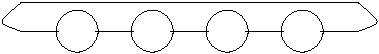
\includegraphics{1Dring}
}
\end{center}
\caption{A 1D ring. The circles represent processors and the lines
represent connections.}
\label{f:1Dring}
\end{figure}

Although the QCDSP has a network connectivity that is a four dimensional 
torus it can also be viewed as a collection of rings. We illustrate
the idea for a two dimensional torus in figure \ref{f:TorusRing}.
Here we can look at a two dimensional torus as a collection of rings in
either the {\em x} or {\em y} directions
\begin{figure}
\begin{center}
\leavevmode
\hbox{%
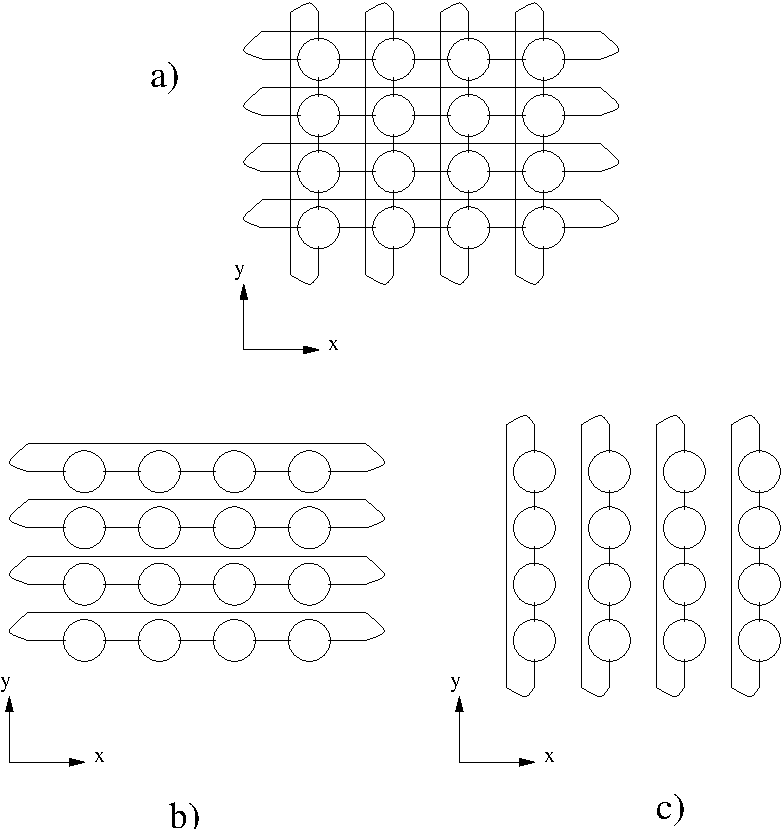
\includegraphics{torusRing}
}
\end{center}
\caption{(a)A 2D torus as a set of 1D rings in the (b) {\em x} direction and (c) the {\em} direction}  
\label{f:TorusRing}
\end{figure}

One general way of programming global reduction algorithms on a 4D mesh
is to perform the operation first on all rings in the {\em x} direction,
then on all the rings in the 'y' direction and so on in the remaining two
directions. 

\subsection{Ring all to all reduction algorithm}
Consider the following reduction algorithm:

Each processor in the ring sets up a buffer to store the result of the
reduction. The result buffer is initialised with the processors own data.

Each ring then transmits its data in one direction along the ring
and receives data from the opposite direction. (We shall refer to these 
as the positive and negative directions respectively). The data that
has been received is combined with the data in the result buffer, to 
generate a new intermediate result..

The process of transmitting the local data in the positive direction
and receiving data from the negative direction and combining it with the
result is repeated until each data item has visited each processor once.
For a ring containing $n$ processors exactly $n-1$ steps are needed.
When all the steps are complete, the result buffer should contain the
final answer.

The process is illustrated for addition in a 4 processor ring in figure
\ref{f:ring_addition}.
\begin{figure}
\begin{center}
\leavevmode
\hbox{%
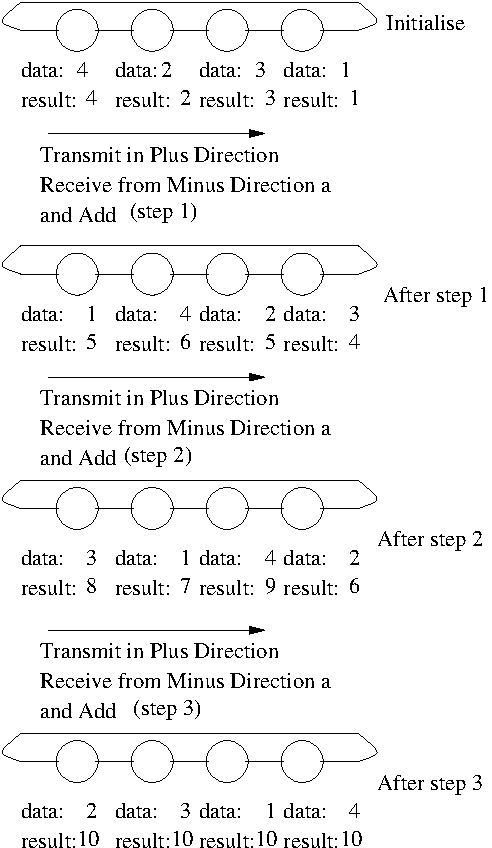
\includegraphics{1Dring_addition}}
\end{center}
\caption{1D Ring Addition Algorithm: At each step data is passed in 
the positive direction (right) and received from the negative direction (left).
The data is then added to the results buffer. After 4-1 = 3 steps
all the processors have the global sum}
\label{f:ring_addition}
\end{figure}

Note that in this particular algorithm, each processor performs the
sum in a different order from its neighbour. This is one of the
reasons why reduction operations need to be associative. Also since
floating point arithmetic is not really associative due to roundoff
errors, it is possible that rounding errors will affect different
processors differently and for a floating point global sum using the
above algorithm, it is possible that the answers on individual
processors are not bit-identical.

This can be a problem for example if one is trying to decide whether one 
meets the stopping criteria for some iterative process based on the result
of a global sum (such as in the case of an iterative solver, where the 
stopping criteria depends on a scalar product). Clearly it is possible
that some processors meet this criteria and some, due to rounding errors
do not. 

The problem can be solved by nominating one processor as the master of
the others. The decision as to whether to stop the solver will then
depend on the result held by the master node. One can either broadcast
the master's result and let each processor make its decision based on
that, or alternatively the master can make the decision and broadcast
it instead in the form of a token, a flag or in some other encoding.
Alternatively one can formulate the global sum so that the results are
guaranteed to be bit identical across all the processors, say by using
a different algorithm where the sum is first reduced to some single root 
processor in all the rings which then transmit the sum back along their
respective rings before going on to the next dimension.

\subsection{Mesh Global reduction algorithm}
As mentioned before, the generalisation of the ring algorithm to the 
mesh is simply to perform the global operation along each ring in
parallel for a given direction, and to repeat this process for 
all directions. 

Figure \ref{f:2DMeshsum} shows the idea for a two dimensional mesh.
\begin{figure}
\begin{center}
\leavevmode
\hbox{%
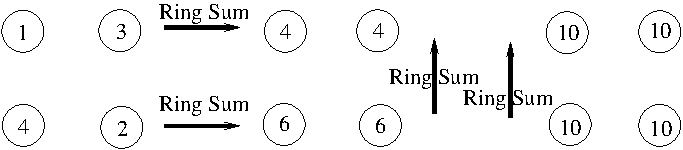
\includegraphics{mesh_sum}
}
\end{center}
\caption{2D Mesh Global sum. First the sum is performed along both 
rings in the horizontal direction. Second it is performed along 
both rings in the vertical direction.}
\label{f:2DMeshsum}
\end{figure}

\subsection{Coding the Routines For the QCDSP}
We show below the QCDSP C++ code for finding the global maximum
using similar the algorithms described above.
\begin{verbatim}
// ------------------------------------------------------
// Include Files
// ------------------------------------------------------
#include <glb.h>
#include <sysfunc.h>

// ------------------------------------------------------
// Macros for picking local min/max
// ------------------------------------------------------
#define max(A, B) ((A) > (B) ? (A) : (B))

// -------------
// Buffer space 
// -------------
static float transmit_buf;
static float receive_buf;
static float max_buf;

// ------------------------------------------------------
// Function glb_max
//
// Argument: A pointer to the local number that is to
// be considered for being the Global Maximum. At the end
// of the function, the pointer points to the global maximum
// ------------------------------------------------------
void glb_max(float * float_p)
{
  // ---------------------------------------------
  // Size of the Processor Grid in each dimension
  // ---------------------------------------------
  int NP[4] = {SizeT(), SizeX(), SizeY(), SizeZ()};

  // ---------------------------------------------
  // Array to hold SCU send and receive directions
  // We will later index into this.
  // ---------------------------------------------
  const SCUDir dir[] = { SCU_TP, SCU_TM, SCU_XP, SCU_XM,
                         SCU_YP, SCU_YM, SCU_ZP, SCU_ZM };
  // ---------------------------------------------
  // Place the local number in the comparison buffer
  // ----------------------------------------------
  max_buf = *float_p;

  // ----------------------------------------------
  // Loop over the processor grid dimensions
  // ----------------------------------------------
  int dim;
  for(dim = 0; dim < 4; dim++) {

      // -----------------------------------------
      // Send our local minimum in the +ve direction
      // (NP[ 2 * dim ]) direction and receive from the
      // -ve (NP[ 2 * dim ]) direction with wraparound
      // at the pe grid boundary. Do this NP - 1 times
      // so that everyone can compare everybody's data
      // in this dimension
      // -----------------------------------------
      transmit_buf = max_buf;

      int tmp;
      for (tmp = 1; tmp < NP[ dim ]; tmp++) {
        // -----------------------------------------
        // Set up the communications handles:
        // -----------------------------------------

        SCUDirArg send(&transmit_buf, dir[ 2*dim ],
                       SCU_SEND, sizeof(float));
        SCUDirArg rcv(&receive_buf, dir[ 2*dim+1 ],
                      SCU_REC, sizeof(float));


        // -----------------------------------------
        // Perform the transfers
        // -----------------------------------------
        SCUTrans(&send);
        SCUTrans(&rcv);

        SCUTransComplete();

        // -----------------------------------------
        // Keep the maximum of what you had and what
        // you just received
        // -----------------------------------------
        max_buf = max(max_buf, receive_buf) ;

        // -----------------------------------------
        // Pass on the received data
        // -----------------------------------------
        transmit_buf = receive_buf;
      }
  }

  // --------------------------
  // Store the global max
  // --------------------------
  *float_p = max_buf;
}
\end{verbatim}
The global minimum and sum routines would follow a similar pattern.

\section{A simple collective communications library}
In a manner similar to the {\em hello\_world} program a simple
global communications library is available on the QCDSP (once 
Bob puts it in place). It can be found in {\tt /qcdsp/sfw/qos.5.3.3/example/glb}.This directory has subdirectories {\tt include}, {\tt lib}, {\tt src} and {\tt test}. There is also a makefile in this directory of which more later.

The {\tt include} directory contains the file {\tt glb.h} which defines
the global communication subroutines. This has to be included in any 
user programs using the {\tt \#include} directive. The {\tt src} 
subdirectory contains the source files for the library plus a makefile
to build the libraries. The {\tt lib} directory is where the compiled
library gets placed after it is built in the {\tt src} subdirectory. 
This is the library that has to be linked with the user code and
is called {\tt glblib.olb} on the QCDSP. Finally, the {\tt test} 
directory contains a simple program that uses the library.

To build the library and the tests, go to the toplevel directory 
and type {\tt make all}. Once this process is finished, you should
find {\tt glblib.olb} in the {\tt lib} subdirectory and an
executable called {\tt glb\_test.out} in the {\tt test} subdirectory.

\subsection{The Library Routines}
The library provides the following routines.
\begin{description}
\item{ {\tt void glb\_sum(float * float\_p)} : \ } This routine
performs a global sum over all the processors. On entry, {\tt float\_p} 
should point to each node's own contribution to the sum. On exit
{\tt float\_p} will point to the result of the global sum. The algorithm
for the sum is as detailed in the last section. The sum is actually 
performed in 64 bits of precision through a user defined type. This
aspect of the operation is completely hidden from the user. At the 
end of the operation the result is rounded back to a 32bit result. 
\item{ {\tt void glb\_max(float * float\_p)} : \ } This routine 
finds the global maximum across all the processors. On entry {\tt float\_p}
points to the each processor's own data. On exit {\tt float\_p} points
to the maximum of these elements. This subroutine was listed explicitly in
the last section.
\item{ {\tt void glb\_min(float * float\_p)} : \ } This routine
finds the global minimum across all the processors. On entry {\tt float\_p}
points to each processor's own data. On exit {\tt float\_p} points
to the minimum of these elements.
\item{ {\tt void glb\_bcast(float * float\_p, int root\_id)} : \ } This 
routine broadcasts the number pointed to by {\tt float\_p} on the node
with unique ID {\tt root\_id} (as determined from {\tt UniqueID()}) to
all the processors.  The broadcast is implemented as a global sum with
node {\tt root\_id} contributing the number to be broadcast at the end
of {\tt float\_p} and all the other nodes contributing 0 to the sum.
\end{description}

We recommend that the reader takes a look at the source code to be
found in the {\tt src} subdirectory to look at the code for the above 
library routines. However most of them are similar to the global
maximum routine listed earlier.

\subsection{Using the Library}
We list below the test program from the {\tt test} subdirectory which 
shows all of the library routines in use. The program first sums the 
unique IDs of all the nodes, then finds the maximum and minimum of these.
Finally it broadcasts the ID's of each processor in turn and sums 
them accross the processor grid. The code is shown below:
{\small
\begin{verbatim}
#include <stdio.h>
#include <stdlib.h>
#include <sysfunc.h>
#include <glb.h>

int main(int argc, char *argv[])
{
  float sum_serial = 0;
  int i;

  // -----------------------------
  // Serial sum of processor ID's
  // -----------------------------
  for(i = 0; i < NumNodes(); i++) {
    sum_serial += (float) i;
  }

  // ----------------------------
  // Put Unique ID into buffer
  // ----------------------------
  static float my_buf = (float)UniqueID();

  // ----------------------------
  // Sum Unique IDs
  // ----------------------------
  glb_sum(&my_buf);

  // ----------------------------
  // Output results
  // ----------------------------
  printf("Serial Sum of IDs = %g  Global Sum = %g\n", sum_serial, my_buf);


  // ----------------------------
  // Find Minimum ID
  // ----------------------------
  my_buf = (float)UniqueID();
  glb_min(&my_buf);

  printf("Minimum Unique ID should be 0. It is %g\n", my_buf);

  // ----------------------------
  // Find Maximum ID
  // ----------------------------
  my_buf = (float)UniqueID();

  glb_max(&my_buf);

  printf("Maximum Unique ID should be %g. It is %g\n", 
         (float)(NumNodes()-1), my_buf);

  // ----------------------------
  // Do some broadcasting
  // ----------------------------
  for ( i = 0; i < NumNodes(); i++ ) {

    // -------------------------------
    // Process I will broadcast its ID
    // to everyone
    // -------------------------------
    if( UniqueID() == i ) {
      my_buf = (float)i;
    }
    else { 
      my_buf =(float) 200;
    }

    // -------------------------------
    // Broadcast with proc i as root: 
    // Should end up with i on each node
    // -------------------------------
    glb_bcast(&my_buf,i);
    
    // -------------------------------
    // Do a global sum on the result 
    // (should be NumElems()*i)
    // -------------------------------
    glb_sum(&my_buf);

    printf("Global sum of buffers should be %g. It is %g\n", 
          (float)(NumNodes()*i), my_buf);

  }
  return(EXIT_SUCCESS);

}
\end{verbatim}
}
When printing the result of each operation the program also prints
out what it expects the real result to be.

Why not compile up the library as indicated before and try out the test
program. On {\tt q\_1}, which is a 64 node development board I got
the following output.
\begin{verbatim}
Serial Sum of IDs = 2016  Global Sum = 2016
Minimum Unique ID should be 0. It is 0
Maximum Unique ID should be 63. It is 63
Global sum of buffers should be 0. It is 0
Global sum of buffers should be 64. It is 64
Global sum of buffers should be 128. It is 128
.
.
.
\end{verbatim}

\subsection{Using the Library in your own programs}
To use the library in your own programs you must do two things.
\begin{itemize}
\item
Firstly, you must include the header file {\tt glb.h} in every
source file that uses the routines.
\item
Secondly, you must link to the library {\tt glblib.olb}. This
may involve having to edit the Makefile. If you dislike this
idea (its not that bad really) simply copy the files ending in
{\bf .C} from the {\tt src} subdirectory into the directory 
you are working in. The default makefiles should compile
them up for you.
\end{itemize}

We shall say discuss compilation and linking in more detail in 
a later chapter. For now suffice it to say that both are done
using the {\tt tcpp} command. 

To include the {\tt glb.h} header file, it is perhaps easiest 
if you leave it in some sensible (Perhaps Bob will leave it
in a sensible place where it can stay forever). You can then do 
one of two things.
\begin{itemize}
\item
You can include it with the directive {\tt \#include "sensible\_path/glb.h"}
where for {\tt sensible\_path}, you should substitute the path
of the sensible place where the header file lives.
\item
You can include it with the directive {\tt \#include <glb.h>}. In this
case you have to make sure that the compiler will look in the sensible
place where the {\tt glb.h} file is by default. You can specify
a list of directories for the compiler to search with the {\tt -i}
compiler flag.
\item
If you feel really unhappy about either of the above options you can
always copy the {\tt glb.h} file into the directory that you are working
in and just include it as {\tt \#include "glb.h"}. This way you need
neither edit the makefile nor mess with compiler flags. Its the 
chicken way out tho' and it may leave you open to having
different versions of the header file in different projects. A real
nightmare...
\end{itemize}
I prefer the latter method personally, as then I only have to 
type the name of the directory in which the file lives once, in
the makefile.

However I do repeat: {\bf If you fear and loath makefiles, do not
panic for we shall clarify them in a later chapter. Until then, just
copy the files from the {\tt src} subdirectory and {\tt glb.h} to the
directory where you are coding and use the default makefiles.}

\section{Summary of Chapter}
In this chapter, we have discussed collective communications.
After outlining some of the most common global communication techniques,
the barrier, the broadcast, gather, scatter and reduction operations
we discussed which of these may be implemented on the QCDSP. 
We then outlined some simple algorithms for performing global reduction
operations on a mesh parallel architecture. Finally, we discussed a
simple library for the QCDSP which defines global sums, maxima and minima
for floating point numbers.

\section{Exercise}
Can you think of more efficient ways of doing global sums on the 
QCDSP ? You should be able to get some ideas from the QCDSP WWW page:
{\tt http://www.phys.columbia.edu/\~cqft/qcdsp.htm} where they describe
the hardware support for global sums. You can also get some ideas
from the book ``Introduction to Parallel Computing'' by Vipin and Kumar
who have gone to great lengths to describe network topologies and 
routing algorithms in use in general parallel computers.



#include<config.h>
CPS_START_NAMESPACE
\chapter{I/O on the QCDSP}
\section{Introduction}
In this chapter we discuss the facilities afforded by QCDSP to perform
input and output (I/O). We consider three aspects: parallel I/O. 
Serial File I/O and I/O to the terminal screen during job runtime.

\section{Parallel I/O}
The QCDSP is a massively parallel supercomputer. Hence there is a high
likelihood (in the case of Lattice QCD it is virtually a certainty) that data
is in some way distributed amongst the numerous QCDSP nodes. The question
then is, how to collect data from the nodes of the QCDSP so that it 
can be written to disk, or alternatively, how to get data from a disk
onto the nodes of QCDSP.

A complication is that on the QCDSP only one processor, to which we
shall refer hereafter as the root node (Motherboard 0, Daughterboard 0,
Unique ID=0) is allowed to actually perform I/O onto a disk on the
host computer. The other nodes can output to what in a UNIX system
would be the {\em standard output} stream. This however is merely a
storage buffer on the memory of the node in question, that has to be
retrieved later using the {\bf qprintf} command (as discussed in
section one).  In fact only node 0 can write to the output stream
during run time in a way that it is echoed on the screen of a user or
can be redirected into a file.  The QOS has no concept of other
streams such as the UNIX {\em standard input} and {\em standard
error}. On the other hand the {\bf qrun} command does allow the
passing of {\em command line arguments} to executing programs as will
be demonstrated later.

Hence, one would think that the best way to read a serial file and
distribute its data amongst processors is for the root node to read
the data and perform various scatter operations to distribute the
data.  Alternatively, saving of data could be done by the root
processor gathering data from the other processors and then writing it
out to disk. This is all very well, as long as the root processor can
hold the whole overall dataset in memory. However, a the amount of
DRAM memory on a single node is quite small, a mere
0.5Mwords\footnote{The wordsize of the DSP is 32bits. The physical
size of a word in DRAM is 40bits of which 8 are reserved for error
correction. Hence 0.5Mwords corresponds to 2Mb of useable
memory. However since everything is word size for the DSP from
characters to floating point numbers it makes more sense to discuss
memory in terms of words than bytes.}. Of this the run time operating
system occupies 128Kwords leaving a mere 384Kwords to the user. This
has to include the user code as well as the user data. Hence one
would be reduced to communicating the data from the nodes to the root node, at 
a rate of one pair of processors at a time. Since the QCDSP has no general
point to point communication routines, this process would have to be implemented
using the usual nearest neighbour communications.

Another alternative would be to use a parallel file system. There is 
such a system currently under development for the QCDSP, however it
is not yet an integral part of the QOS, and hence it shall not be 
discussed any further here. 

The question then remains: How can parallel data be loaded and
distributed in a straightforward manner on the QCDSP, and how can the
data be saved from amongst all the processors into one file. On the
QCDSP this is done via the {\bf qread} and {\bf qload} commands using
objects called Node Tagged Tiles (NTFs). An NTF is a single serial
file written in ASCII (can we do binary Bob?) that contains the
relevant data from all the nodes of the QCDSP. Preceeding the data
from a given node is a tag identifying the node which is to host the
data. We will discuss their detailed. One can then develop
workstation tools to convert between these NTFs and regular serial
files. For those readers who intend to load and save lattices to and
from the Columbia Physics environment (stored in the Gauge Connection
Archive Format\footnote{See the Gauge Connection Web site {\tt http://qcd.nersc.gov}}) QOS provides the more specialised commands: {\bf
qload\_lattice} and {\bf qunload\_lattice}. 

\section{Parallel I/O with NTFs, qread and qload}
When a QCDSP program exits and the QOS returns control to the front end,
the memory space of the program prior to exit is left untouched. The 
{\bf qread} and {\bf qunload\_lattice} routines access this memory directly
and dump a user specified number of data blocks from a 
user specified memory address to a file. The {\bf qread} command can 
dump either to a screen or to a NTF. Its output is always in ASCII
format. The {\bf qunload\_gauge} command writes directly to a file
in the Gauge Connection Archiver format.

The {\bf qload} command can be used to place data into processor
memory prior to execution. It works in two ways:
\begin{itemize}
\item
One can specify a memory address and the value to be placed there
as command line arguments to {\bf qload}. The {\bf qload} command will
then place the given value into the given memory address. The user program
can then be run. It can be passed the address of the data and the number
of data blocks as command line parameters. Once running the code can set
a pointer to the given address and copy the relevant data to some 
of its own memory.
\item
The qload command can be given the name of an NTF. The NTF contains
the starting address and the number of blocks for the data,as well as the
data itself, for each processor.
The program can access the data by setting a pointer to the  address.
which can be passed as a command line argument.
\end{itemize}

The {\bf qload\_lattice} command works similarly to the {\bf qload}
command. However the gauge connection format lattice file is not node tagged. 
The user passes the address where the first lattice site is to be placed
on each processor, and the name of the lattice file to the {\bf qload\_lattice}
command. The lattice sites are then placed into processor memory. A 
lattice object can then be instantiated giving the address of the first
lattice element to the lattice object constructor.

Of course in both the above cases dealing with {\bf qload}, the data
may be copied directly into the program data area. This can be made to
be safe, as the linker produces resolved code. This means that the
code produced by the linker will not be relocated afterwards at the
start of execution. Hence one can print out the address of a declared
array in the program, safe in the knowledge that the next time the
program will run, the array will have the same address. {\bf WARNING:
This behaviour is peculiar to the QCDSP.} Furthermore one can glean
information about the addresses of symbols after the compilation and
linking by looking through the linker map file. We shall discuss this
in more detail in the next chapter.

Before describing the details of the NTFs, and giving examples of using
the {\bf qload} and {\bf qread} lattices we should say a few words about
the organisation of memory on each node of the QCDSP. Even before that
here is possibly our most severe {\bf WARNING: The command {\bf qload}
can (and will) if incorrectly used, overwrite memory used by  the QOS 
operating system. This can have UNPREDICTABLE results ranging from no
effect, through subtle bugs, to system crashes. Be careful with it!!!}.

\subsection{The DSP memory Map Part 1}
The complete memory map of the DSP is quite complicated. In this section
we shall just describe a small part of it, that pertains to compiling
and running programs. 

The memory addresses on a single QCDSP node can range from 000000 to 
FFFFFF (remember your hexadecimal numbers?). This space however is 
not all memory and some of it is not accessible. In particular 
the 0.5Mwords of DRAM are mapped between addresses 001000
to 07FFFF. The addresses from 000000 to 001000 are not accessible by 
the DSP in the mode it is used. Memory addresses 080000 and upwards
are special. They either contain views of the data in real memory
(ie that between 000000 and 07FFFF) for use by other hardware such
as the circular buffer, or they contain the memory mapped
images of the DSP internal memory and control registers. We may
deal with some of these latter in the chapter on optimisation.

The run time operating system starts at 060000 and can stretch
until 07FFFF. Consequently {\bf only the memory area from address
001000 to 05FFFF (inclusive) is available for user programs.}

This rough sketch of the memory map is illustrated in figure 
\ref{f:MMap1}.

\begin{figure}[h]
\begin{center}
\leavevmode
\hbox{
\begin{tabular}{|c|l|} 
\hline 
{\bf Address Range} & {\bf Function } \\
\hline
D00000 -- FFFFFF & \begin{tabular}{l} Used on node 0. Unused elsewhere. Generally reading \\ from or writing to here will cause the DSP to hang \end{tabular} \\
\hline 
880000 -- CFFFFF & \begin{tabular}{l} Various images of the 0.5Mwords of DRAM between \\  000000 -- 07FFFF for use of the circular buffer \end{tabular}  \\ 
\hline
820000 -- 87FFFF & Not used \\
\hline 
810000 -- 81FFFF & Addresses of registers for controlling the NGA \\
\hline
800000 -- 80FFFF & Inernal DSP Memory and control register area \\
\hline 
080000 -- 7FFFFF & \begin{tabular}{l} Images of 0.5Mwords of DRAM between 000000 -- 07FFFF \\  for use of the circular buffer \end{tabular} \\
\hline 
{\bf 060000 -- 07FFFF} & {\bf 128Kwords of DRAM reserved for Operating system} \\
\hline
{\bf 001000 -- 05FFFF} & {\bf 384Kwords of DRAM for User programs} \\
\hline
 000000 -- 000FFF & Inaccessible \\ \hline 
\end{tabular}}
\end{center}
\caption{Memory Map of a DSP node. The Memory is word addressed.}
\label{f:MMap1}
\end{figure}

\subsection{Program Images} 
If you have been using the default Makefiles you should find that 
usually a file is produced with the {\bf .map} suffix alongside your
executable. In the case of the ``Hello Wold'' program this file would
be called something like {\tt hello\_world.out}. (The default makefile
always names output files after the directory in which the source files live).

The map file is quite useful as it tells you about how much memory 
your program has allocated statically during compilation, allowing you
to figure out how much space you have to {\em qload} your NTF into. 

Your program, as far as the linker is concerned consists of 6 parts 
of which 3 are negligible. The important three parts go by the names of
{\em data segment}, {\em binary stack segment (BSS)} and the {\em text segment}.
The unimportant parts are there mostly to supply information to debugging tools.
In the case of the Tartan Linker these are called the {\em debug directives} 
segment, the {\em debug strings} segment and the {\em debug source location}
segment. You need not care about these right now. Unless you switch on the
option on the compiler to produce debugging information, these latter three
segments will be empty.

The BSS contains amongst other things your runtime stack, on 
which C++ allocates automatic variables. The data segment is used
to hold various constant data items and the text segment holds the
actual machine level instructions of your program. Any free memory outside
these segments is unallocated and should be placed onto the heap when your
program starts running so that you can allocate memory from it dynamically.

The map file tells you about how your program is laid out in memory.
It starts off by telling you how much space is allocated to the various
segments. For example here are some excerpts from my {\bf hello\_world.map}
file

{\small
\begin{verbatim}
Tartan Linker, SPARC/C40, v5.1.0        4/4/100 13:33:37                Page   1
Copyright (c) 1986-1992 by Tartan, Inc., All Rights Reserved


Allocation to Output Section ".bss" in module *unnamed* in file
"/homeqs0/bj/hello_world/hello_world.outtof"

  Offset   Length               Input Section

    1000      162       "TL.Init" in module "main" in file
                        "/homeqs0/bj/hello_world/main.tof"
    1162        1       ".bss" in module "qcdsp_tcroot" in file
                        "/usr/local/tartan/v2.1/etc/qcdsp_v5.3.3/tcrt30bs.olb"
    1163       21       "OWN" in module "inifin" in file
                        "/usr/local/tartan/v2.1/etc/qcdsp_v5.3.3/tcrt30bs.olb"
    1184     1000       ".stack" in file
                        "/usr/local/tartan/v2.1/etc/qcdsp_v5.3.3/link.lcf"

  Total Allocation = 1184 (hex)

Allocation to Output Section ".data" in module *unnamed* in file
"/homeqs0/bj/hello_world/hello_world.outtof"
  Offset   Length               Input Section

    2184        D       "DEFALT" in module "qcdsp_tcroot" in file
                        "/usr/local/tartan/v2.1/etc/qcdsp_v5.3.3/tcrt30bs.olb"
    2191      16E       ".cinit" in file
                        "/usr/local/tartan/v2.1/etc/qcdsp_v5.3.3/link.lcf"

  Total Allocation = 17B (hex)

Allocation to Output Section ".text" in module *unnamed* in file
"/homeqs0/bj/hello_world/hello_world.outtof"

  Offset   Length               Input Section

    22FF       6C       "_main" in module "main" in file
                        "/homeqs0/bj/hello_world/main.tof"
    236B       2A       ".text" in module "sysfunc" in file
                        "/usr/local/tartan/v2.1/etc/qcdsp_v5.3.3/tcio30bs.olb"
    2395       56       ".text" in module "qcdsp_tcroot" in file
                        "/usr/local/tartan/v2.1/etc/qcdsp_v5.3.3/tcrt30bs.olb"
    23EB       26       "dbgrpc" in module "tcrpc" in file
                        "/usr/local/tartan/v2.1/etc/qcdsp_v5.3.3/tcrt30bs.olb"
    2411        7       ".text" in module "tcrpc" in file
                         "/usr/local/tartan/v2.1/etc/qcdsp_v5.3.3/tcrt30bs.olb"
    2418       32       ".text" in module "tcinit" in file
                        "/usr/local/tartan/v2.1/etc/qcdsp_v5.3.3/tcrt30bs.olb"
    244A       22       "_exit" in module "inifin" in file

Tartan Linker, SPARC/C40, v5.1.0        4/4/100 13:33:37                Page   2
Copyright (c) 1986-1992 by Tartan, Inc., All Rights Reserved

                        "/usr/local/tartan/v2.1/etc/qcdsp_v5.3.3/tcrt30bs.olb"
    246C        2       "__main" in module "inifin" in file
                        "/usr/local/tartan/v2.1/etc/qcdsp_v5.3.3/tcrt30bs.olb"

  Total Allocation = 16F (hex)
\end{verbatim}
}
You can clearly identify the three sections for the BSS, data and text segments.
(They are referred to as output sections {\tt .bss}, {\tt .data} and {\tt .text}.)

Following all this information is a summary of the output sections that
tells you the total amount of memory allocated to each individual section.
In my {\bf hello\_world.map} file this looks like:
{\small
\begin{verbatim}

                Output Sections

Section List for Module *unnamed* in file
"/homeqs0/bj/hello_world/hello_world.outtof"

Number  Physical   Start   Length  Kind         Access  Name
  1                  1000     1184 data                 ".bss"
  2                  2184      17B constant             ".data"
  3                  22FF      16F code                 ".text"
  4                     0        0 debug                "debug_directives"
  5                     0        0 debugstring          "debug_strings"
  6                     0        0 line number          "debug_source_location"
}
\end{verbatim}}
This is perhaps the most useful piece of information in the map file.
It tells me the starting addresses of each of my program segments and 
how long they are (the columns Start and Length). I can see from here that 
my program uses memory from address 001000 to 0022FF + 16F = 00246E inclusive.
Hence if this program were to take any input via {\tt qload} I would 
know that it should be safe to fill up memory from 0246F upwards.

The remainder of the map file lists every single symbol used in your
program. You may find it amusing to see how few of them you recognise.
Here are some symbols from the {\bf hello\_world.map} file that you 
may recognise
{\small
\begin{verbatim}
Kind  Offset Sect Virtual Physical      Name
          6F   3     236E          "_CoorT"
          70   3     236F          "_CoorX"
          71   3     2370          "_CoorY"
          72   3     2371          "_CoorZ"
          93   3     2392          "_CurrentStatus__FiPc"
 W        97   3     2396          "_c_int00"
          6D   3     236C          "_DbNum"
         14C   3     244B          "_exit"
         14B   3     244A          "_exit$LAJ"
          8E   3     238D          "_fclose"
          8C   3     238B          "_fopen"
          8D   3     238C          "_fprintf"
          91   3     2390          "_HdwCheck__Fi"
          94   3     2393          "_InterruptExit__FiPc"
           1   3     2300          "_main"
           0   3     22FF          "_main$LAJ"
          6C   3     236B          "_MbNum"
          90   3     238F          "_NodeStatUpdate__Fv"
          77   3     2376          "_NumNodes"
          7C   3     237B          "_printf"
\end{verbatim}
}
You may be worried here that at startup, spurious memory allocation
might overwrite your qloaded data. This is not a worry here as the
map file includes the heap area as well. Hence if you place something
above the last address in the map file, it is guaranteed that it 
will not be malloced over. 

You can configure the size of the heap and other program layout
options in a file called the Linker Control File. If you do not 
use one of these the program will be linked under the control of 
a default linker control file which allocates a pitifully small heap.
(0x1000 words). Hence when you come to code bigger projects you
will have to allocate the heap yourself in your own LCF. This will
involve a partitioning of the available memory between room for 
your program, data you intend to allocate dynamically (heap) and data
you intend to qload. 

The standard procedure is to qload data very high in memory, just
below the operating system. Suppose you have data of say 32Kwords per
processor (0x8000 words (hex)). The operating system starts at address
0x060000 and so you might want to load the data to 0x06000 - 0x008000
= 0x058000. Then you can set up your LCF so that your program cannot
extend beyond 0x057fff (heap included). It is of course prudent to
leave a bit of room here and there in case you modify your program. In
the words of investment brokers ``The size of your program can go down
as well as up.''.

We will discuss linking, program sections and control files in more detail
in the next chapter about compiling and linking.

\subsection{Node Tagged File Formats}
We now discuss node tagged files.
Node tagged files are written in ASCII and contain hexadecimal numbers.
Although this can cause the files to be large and slow to read and write,
it does have the advantage that the files are readable without needing
specialist dump programs.

The file format consists of one hexadecimal entry on each line 
written in ASCII. The structure of the entries is given below.
below. Each heading and sub--heading corresponds to an entry 
in the NFT.
\begin{description}
\item{\bf A 'Magic Number' : \ } -- This is an integer for identifying
which of the 3 types of node tagged files one is dealing with. The
three types are: \begin{description} \item{tree \ } -- the nodes are
tagged according to their position on the SCSI tree by a pair of
numbers (M,D) representing the node's motherboard and daughterboard
number respectively. Each of these numbers corresponds to a new entry
on a new line in the NTF. The magic number for this mode is 2.  This
is the 'default' tag mode. Node tagged files in this format usually
have a {\bf .tree} file suffix.  \item{Machine 4D \ } -- the nodes are
tagged with their 4D coordinates within the processor grid (A
four-tuple of integers, each of these on a new line in the NTF). The
magic number for this tag mode is 3. Node tagged files in this mode
usually have a {\bf .m4d} file suffix.  \item{Physics 4D \ } -- to all
intents and purposes this format the same as the machine 4D. Nodes are
tagged by their 4D coordinates. The meaning of fields however is
different. In terms of machine coordinates, everything is
fixed. However the machine coordinates can be re mapped at boot time to
interchange the order of coordinates. Hence (T,X,Y,Z) coordinates can
be re mapped to (X,Y,Z,T) coordinates etc. The machine 4D file never
changes the data layout. However the physics 4D file can shift the
data around depending on the current 4D mapping. The magic number for
this mode is 4. Node tagged files in this mode usually have the {\bf
.p4d} file suffix.  \end{description}
\item{\bf A sequence of Node Records} -- for each node in the processor there is
a record. A record has the following structure.
	\begin{description}
	\item{A Node Tag \ } -- A tag identifying the node. For the tree structure this consists of the  motherboard number followed by the daughterboard
number. For the 4D modes this is a four tuple of integers identifying the
4D coordinates of the node.
	\item{The number of blocks for the Node \ } -- An integer indicating
how many blocks of data are to be loaded into the memory of the node (Hexadecimal without leading 0x)
	\item{Base Address \ }--  A hexadecimal address (without leading 0x) specifying the location in memory where the first data item is to be placed.
	\item{Data Blocks \ } -- An ASCII representation of each data block. In the case of integers this is quite readable. In the case of floats it is not
	\item{A terminator \ } -- An ASCII zero follows the final record as a 
record termination signal.
	\end{description}
\end{description}

The formats of the NTFs, the magic numbers, node tags and file extensions
are summarised in figures \ref{f:NTFStructure}, \ref{f:NTFRecStructure} 
and \ref{f:NTFTypeSummary}.

\begin{figure}[ht]
\begin{center}
\leavevmode
\hbox{%
\begin{tabular}{|c|}
\hline
Magic Number \\
\hline
Record No 1 \\
\hline
Record No 2 \\
\hline 
$ \vdots $ \\
\hline
Last Record \\
\hline
\end{tabular}}
\end{center}
\caption{Structure of a Node Tagged file -- Components are sequential in an ASCII file. Each component starts on a new line}
\label{f:NTFStructure}
\end{figure}

\begin{figure}[ht]
\begin{center}
\leavevmode
\hbox{%
\begin{tabular}{|c|} \hline
Node Tag \\
\hline 
$n$ -- Number of blocks \\
\hline 
Base Address \\
\hline 
block[0] \\
\hline
block[1] \\
\hline
$\vdots $ \\
\hline
block[ $n-1$ ] \\
\hline
0 (terminator) \\
\hline
\end{tabular}}
\end{center}
\caption{Structure of a Node tag record -- Each component is in ASCII on a new line}
\label{f:NTFRecStructure}
\end{figure}

\begin{figure}[ht]
\begin{center}
\leavevmode
\hbox{%
\begin{tabular}{|c|c|c|c|}
\hline 
{ \bf File Type}  & {\bf Magic Number} & {\bf Node Tag Components} & {\bf File Suffix } \\
\hline
Tree & 2 & \begin{tabular}{c} Motherboard No \\ Daughterboard No \end{tabular} & {\tt .tree} \\
\hline
Machine 4D & 3 & \begin{tabular}{c} T Coordinate \\ X Coordinate \\ Y Coordinate \\ Z Coordinate \end{tabular} & {\tt .m4d} \\
\hline
Physics 4D & 4 &  \begin{tabular}{c} T Coordinate \\ X Coordinate \\ Y Coordinate \\ Z Coordinate \end{tabular} & {\tt .p4d} \\
\hline
\end{tabular}}
\end{center}
\caption{Magic Number Node Tag and File Suffix information for the three node tagged file types. The magic number is the first number of any node tagged
file. It should be an ASCII integer on the first line. The node tag
fields should be ASCII integers. Each entry should take a separate
line in the file.}
\label{f:NTFTypeSummary}
\end{figure}

Perhaps the easiest way of creating a node tagged file is to dump
some memory from a program. We now proceed to demonstrate how this is done.

\section{Creating Node Tagged files using qread}
Consider the following little program:
{\scriptsize
\begin{verbatim}
CPS_END_NAMESPACE
#include <stdio.h>
#include <stdlib.h>
#include <strings.h>
#include <sysfunc.h>
CPS_START_NAMESPACE


int main( int argc, char *argv[] ) 
{
  float i[5]={1.0,2.0,3.0,4.0,5.0};

  printf("The address of i is %x and its length is %x blocks\n",
           i, 5*sizeof(int));

  return(EXIT_SUCCESS); 
}
\end{verbatim}
}

The code itself does nothing, but prints out the address of the first 
element of the floating point number array {\tt i}. We can use this 
information to dump the floating point array into an NTF.

\subsection{Setting options for qread}
There are several options that allow you to control how you want to
perform the dump. For example, you can dump to a screen or a named 
file. You can dump into an NTF of either the tree, machine 4D or 
of the physics 4D variety. You can rewrite an existing file or 
append to it. These options are set by the following {\tt qcsh} commands:
\begin{description}
\item{{\tt qset\_read\_output\_filename} : \ } This command takes one 
argument which is the name of the file you want {\tt qread} to 
dump your data to.
\item{{\tt qset\_read\_output\_file\_access} : \ } This command 
takes a single argument to determine whether you wish to use
the append write mode or the overwrite mode. The possible arguments
are 
	\begin{description}
	\item{\tt a \ } -- append mode
	\item{\tt w \ } -- write mode
	\end{description}
\item{{\tt qset\_read\_output\_select } : \ } This command determines 
whether you wish your dump to go to the screen or to a named file
(that you have to name using {\tt qset\_read\_output\_filename}.
It takes a single argument. The argument can have the following values:
\begin{description}
	\item{\tt f \ } -- dump to named file
	\item{\tt s \ } -- dump to screen
\end{description}
\item{{\tt qset\_read\_output\_tagged} : \ } This command determines
the tag type of your dump file. It takes a single argument. Allowed 
argument values are
\begin{description}
\item{ \tt no \ } -- Do not node tag the file. I do not describe the
results of this option. 
\item{ \tt yes \ } -- Place node tags into file. Use default tag mode (tree).
\item{ \tt tree \ } -- Use tree tag mode.
\item{ \tt m4d \ } -- Use machine 4D tag mode.
\item{ \tt p4d \ } -- Use physics 4D tag mode.
\end{description}
\end{description}

\subsection{Using qread to dump to a file}
Let us now have a go at dumping the floating point array in the previous
code snippet. Create a directory called {\tt dump} somewhere and copy
the program listing above into a file named {\tt main.C} (alternatively
the directory may be available under {\tt <QOS\_VERS>/examples/ParIO/dump}).

If you are doing things by hand, you probably want to copy a 
default {\tt Makefile} from the {\tt hello\_world} directory and
build the program by typing {\tt make}. This should produce a program
called {\tt dump.out}. If you are copying the directory structure it should
have a Makefile with it.

Boot the machine and enter the QC-Shell.I will use the machine {\tt
q\_1}.  Now let us suppose that we want to dump the {\tt float} array
from each PE into a file called {\tt foo}.  Let us try first with the
tree node tag mode. We set up the dump using the following {\tt qcsh}
commands (I removed the Qdaemon responses to save space).
\begin{verbatim}
(dump: qcsh[q_1])% qset_read_output_select f
(dump: qcsh[q_1])% qset_read_output_filename foo.tree
(dump: qcsh[q_1])% qset_read_output_file_access w
(dump: qcsh[q_1])% qset_read_output_file_tagged tree
\end{verbatim}

Now run the program using {\tt qrun} as before (Qdaemon messages removed):
\begin{verbatim}
(dump: qcsh[q_1])% qrun dump.out
The address of i is 105d and its length is 5 blocks
\end{verbatim}
Now I can dump to the NTF using {\tt qread}. This command takes the 
base memory address and the number of blocks as two hexadecimal numbers
respectively (without the leading 0x in terms of notation). I dump the 
array with the command (of course you may find a different base 
address to 105d in which case you have to substitute that in what
follows) :
\begin{verbatim}
(dump: qcsh[q_1])% qread 105d 5
\end{verbatim}
to which the machine responds:
\begin{verbatim}
Qdaemon state is:
        qdaemon task is READ
        qdaemon abort no and resume no
        QCDSP synchronous
        All nodes selected with SCSI tree coordinates

Qdaemon:  Parameters for read from QCDSP:
        Read address:           0x105d
        Read blocksize:         0x5
        Filename:               foo.tree
        File access:            write
        File format:            node tagged tree


Qdaemon state is:
        qdaemon task is READ
        qdaemon abort no and resume no
        QCDSP synchronous
        All nodes selected with SCSI tree coordinates
\end{verbatim}
and the file {\tt foo.tree} magically appears in the directory.

We can actually look at the {\bf foo.tree} file. My one looks like:
{\small
\begin{verbatim}
2
0
0
5
105d
0
1000000
1400000
2000000
2200000
0
0
1
5
105d
0
1000000
1400000
2000000
2200000
0
.
.
.
0
3f
5
105d
0
1000000
1400000
2000000
2200000
0
\end{verbatim}
}

You can clearly see the structure here. The first number in the file
is the magic number 2. The next two are the node tag for the tree
coordinates.  These are motherboard and daughterboard identifiers (the
last daughterboard identifier is 3f which is hex for 63.  This is
because I am using only a 64 PE single motherboard machine).  After
this you have the number of blocks -- 5 -- followed by the base
address 105d. You have 5 lines of data. They are the hex
representations of the bit pattern that makes up our 5 floating point
numbers. Finally you have a 0 as an end of record marker.

\section{Loading data with qload}
\subsection{Poking individual words with qload}
The command {\tt qload} allows you to either load node tagged files or to place
individual words into memory. Like qread it also has a number of options
you can set. In this subsection we discuss first how to place individual 
words in memory (ever hear of the POKE keyword in BASIC? This is kind of
the same stuff).

The incantation to load a word into a particular location in memory is
of the format 
\begin{verbatim}
qload <address> <data>
\end{verbatim}
where both the address and the data are hexadecimal values. For example
to load the value 5 into the memories of all the processors at address
04EFFF I would type a magic incantation like:
\begin{verbatim}
(qcdhost/homeqs0/bj/QCDSP/IO/load: qcsh[q_1])% qload 04EFFF 5
\end{verbatim}

To that this has worked consider the following program:
{\scriptsize
\begin{verbatim}
CPS_END_NAMESPACE
#include <stdio.h>
#include <stdlib.h>
#include <strings.h>
#include <sysfunc.h>
CPS_START_NAMESPACE

int main( int argc, char *argv[] )
{
  // -----------------------------------------------
  // qload will put (poke?) the distributed memory
  // into the data. User passes in the address the
  // data has been load to through command line
  // arguments
  // -----------------------------------------------
  int *loaded_ints;
  int nblocks;

  // -----------------------------------------------
  // Check command line arguments
  // -----------------------------------------------
  if( argc != 3) {
    printf("Usage: qrun load.out <base address(in hex)> <no of blocks(in hex)>\n
");
    return(EXIT_FAILURE);
  }

  // -------------------------------------------------------------
  // Convert HEX base address string into an integer pointer value
  // and point loaded_ints there
  // -------------------------------------------------------------
  loaded_ints = (int *)strtol(argv[1],  (char **)NULL, 16);

  // -------------------------------------------------------------
  // Convert no_of_blocks string into an integer value
  // -------------------------------------------------------------
  nblocks = (int)strtol(argv[2], (char **)NULL, 16);

  // -------------------------------------------------------------
  // Confirm values to the user
  // -------------------------------------------------------------
  printf("%x (%d) blocks of data at %x\n", nblocks, nblocks,
         (unsigned int)loaded_ints);

  // -------------------------------------------------------------
  // Print back the data
  // -------------------------------------------------------------
  for(int i = 0; i < nblocks; i++) {
    printf("%d ",loaded_ints[i]);
  }
  printf("\n");

  return(EXIT_SUCCESS);
}
\end{verbatim}
}

This program basically checks your {\tt qload}.You need to  pass it the base
address to where you have loaded your data as well as the number of blocks 
comprising the data. These are passed on to the program as strings
in the {\tt argv} array, so first we have to convert them to addresses.
This is done using the {\tt strtol} function call which converts a 
string to a long integer.

The number 16 in the third argument tells {\tt strtol}\footnote{{\tt
strtol} is a very useful function. For details look at the {\tt man}
page in section 3 of the manual} that the string is supposed to
represent a hexadecimal number. We set a pointer {\tt loaded\_ints} to
the results of the string conversion, in other words to our base
address.

We then also need to convert the number of blocks to an integer. This is
done by the second call to {\tt strtol}. 

After confirming to the user that the input values have been read correctly,
the code proceeds to list the specified number of words from the base 
address, treating them as integers and prints them to the screen.

Compile up this little program. You should also find it already written
on the QCDSP in the directory {\tt <QOS\_VERS>/examples/ParIO/load} with
a suitable default Makefile (Replace this with wherever we put it...)
Now lets have a look in the map file (in my case its called {\tt load.map}):
{\scriptsize
\begin{verbatim}
                Output Sections

Section List for Module *unnamed* in file
"/homeqs0/bj/QCDSP/intro/IO/load/load.outtof"

Number  Physical   Start   Length  Kind         Access  Name
  1                  1000     110C data                 ".bss"
  2                  210C      102 constant             ".data"
  3                  220E      26F code                 ".text"
  4                     0        0 debug                "debug_directives"
  5                     0        0 debugstring          "debug_strings"
  6                     0        0 line number          "debug_source_location"
\end{verbatim}
}
This tells me that it is safe for me to load things above the address 220E+26F = 247D. However it is good practice to load things high in the memory so I will
load the data to 05FFE0. I do this by typing
\begin{verbatim}
(qcdhost/homeqs0/bj/QCDSP/intro/IO/load: qcsh[q_1])% qload 05FFE0 5
\end{verbatim}
Now I run my program 
\begin{verbatim}
(qcdhost/homeqs0/bj/QCDSP/intro/IO/load: qcsh[q_1])% qrun load.out 05FFE0 1
\end{verbatim}
The computer replies
\begin{verbatim}
1 (1) blocks of data at 5ffe0
5 
\end{verbatim}
on all the processors.

\subsection{Loading NTFs using qload}
The qload command can also be used to load NTFs. Since all the information
about the data is in the NFT (processor coordinates, base addresses, number of blocks and the actual data) is present in the NTF file. There is no need
to specify these. The command is simply
\begin{verbatim}
qload <filename>
\end{verbatim}
The command can identify the tag type used in the file from the magic number.

Consider the little program above but now converted to dump floats instead 
of ints:
{\scriptsize
\begin{verbatim}
CPS_END_NAMESPACE
#include <stdio.h>
#include <stdlib.h>
#include <strings.h>
#include <sysfunc.h>
CPS_START_NAMESPACE

int main( int argc, char *argv[] )
{
  // -----------------------------------------------
  // qload will put (poke?) the distributed memory
  // into the data. User passes in the address the
  // data has been load to through command line
  // arguments
  // -----------------------------------------------
  float *loaded_floats;
  int nblocks;

  // -----------------------------------------------
  // Check command line arguments
  // -----------------------------------------------
  if( argc != 3) {
    printf("Usage: qrun load.out <base address(in hex)> <no of blocks(in hex)>\n
");
    return(EXIT_FAILURE);
  }

  // -------------------------------------------------------------
  // Convert HEX base address string into an integer pointer value
  // and point loaded_ints there
  // -------------------------------------------------------------
  loaded_float = (float *)strtol(argv[1],  (char **)NULL, 16);

  // -------------------------------------------------------------
  // Convert no_of_blocks string into an integer value
  // -------------------------------------------------------------
  nblocks = (int)strtol(argv[2], (char **)NULL, 16);

  // -------------------------------------------------------------
  // Confirm values to the user
  // -------------------------------------------------------------
  printf("%x (%d) blocks of data at %x\n", nblocks, nblocks,
         (unsigned int)loaded_ints);

  // -------------------------------------------------------------
  // Print back the data
  // -------------------------------------------------------------
  for(int i = 0; i < nblocks; i++) {
    printf("%f ",loaded_floats[i]);
  }
  printf("\n");

  return(EXIT_SUCCESS);
}
\end{verbatim}
}

We can use this to load our floating point NFT ({\tt foo.tree}) that 
we created before, but first another word about memory.

\subsection{Manual Data Relocation}
Usually it will be the case, that a program loads an NTF at the start
to a memory location, then processes it and then dumps it at the end.
In this case the address in the node tag file is fine both for reading 
and dumping. However we are now at an advanced stage, where one program
produced the NTF but another program wants to load it.

 In the program that made the NFT, the data was in a standard
statically defined array that started (in my case) at address
105d. Now however, we want to load it into a different program.  After
converting the dump program to deal with floats, a quick look at the
map file tells me that memory is still free from above 247D -- this is
a consequence of the fact that the {\tt int} on the DSP is the same
size as the {\tt float}. It is desirable to load the data to a high address,
say 05e000. This can be achieved by editing the NTF and replacing 105d
everywhere with 05e000. In my case the it is simply a question of a global
edit. This is one of the advantages of the NTF being in ASCII format.

\subsection{Example of loading an NTF}
So, edit the previous program to deal with floats as I have done above.
Edit your file {\tt tree.foo} replacing the base addresses everywhere with
05e0000. Load the NTF using the command
\begin{verbatim} 
(qcdhost/homeqs0/bj/QCDSP/intro/IO/load: qcsh[q_1])% qload foo.tree
\end{verbatim}
and run the program, it should probably be called {\tt load.out}:
\begin{verbatim}
(qcdhost/homeqs0/bj/QCDSP/intro/IO/load: qcsh[q_1])% qrun load.out 05e000 5
\end{verbatim}
The computer should reply:
\begin{verbatim}
5 (5) blocks of data at 5e000
1.000000 2.000000 3.000000 4.000000 5.000000 
\end{verbatim}
on all the processors.

\subsection{Setting up qload options}
You should now be able to use {\tt qload} to load parallel data. However
just like the case of {\tt qread} there are some options that you can
set. These allow you to specify the filename to {\tt qload} or simply 
just the address and value to {\tt qload} (for poking single data). Then 
you can use {\tt qload} with no arguments at all. The commands to set 
the options are
\begin{description}
\item{ {\tt qset\_load\_select} : \ } Specifies whether {\tt qload} should
read from a file or from the screen. The command can have up to 1 argument
whose value is either {\tt file} or {\tt screen} (alternatively {\tt f} or
{\tt s} respectively). If no arguments are given, the current value of
the option is shown. I generally found that this option reset itself to 
file every time {\tt qload} is invoked with an explicit filename.
\item{ {\tt qset\_load\_screen} : \ } Specifies an address and a data 
item. This option sets things up so that a subsequent call to {\tt qload} 
will load the specified data to the specified address. The command can 
have either  two arguments or none. Invoking the command with no arguments
causes it to print the current values for the address and the data value.
When the command is invoked with two arguments, the meaning of the arguments
are
\begin{description} 
\item{\tt address \ } specifies the address to load to.
\item{\tt data value \ } specifies the value of the data to be loaded.
\end{description}
Notes:
\begin{itemize}
\item 
The following are equivalent: {\tt qload <address> <value>} and {\tt qset\_load\_select s ; qset\_load\_screen <address> <value> ; qload}.
\item
If one selects to load from the screen, and sets the address and value and
then invokes {\tt qload <filename>}, then {\tt qload} will switch to 
reading from the file instead. If one has set a filename to load from 
using {\tt qset\_load\_filename} and has switched {\tt qload} to read from 
file using {\tt qset\_load\_filename file}, if one now executes {\tt qload <address> <value>} then {\tt qload} will switch to screen mode and the last option
will be valid.
\end{itemize}
\item{\tt qset\_load\_filename : } This command sets the name of the file
that qload will use to load data from. It can have either one or no arguments.
If the command is invoked with no arguments it will echo the current value
of the filename. If invoked with one argument the argument, the argument
should be the name of the file to load from.
Note: The following are equivalent: {\tt qload <file>} and {\tt qset\_load\_select file ; qset\_load\_filename <file> ; qload }.
\end{description}

\section{Digression for Lattice Folk}
There are two specialised commands to load and unload lattice gauge fields to
and from the QCDSP. These are, as mentioned previously {\tt qload\_lattice}
and {\tt qunload\_lattice}. Before describing these I should say a few 
words about the lattice file format.

\subsection{Gauge Connection Format}
Currently NERSC provides an archive area called the {\tt Gauge Connection}.
They use a particular format for lattices there. This format consists
of a header section and a data section. The header section consists of
a whole lot of fields. This is useful for keeping track of where the 
lattices came from. The header file also keeps information about the
average plaquette to assist in validation.

The command {\tt qload\_lattice} simply takes a configuration in the NERSC
archive and loads it into memory at a user supplied starting address.
For example, prior to running a certain piece of code. I have obtained
(actually output from another program) a lattice called {\tt lattice.ieee.full }. The {\tt .ieee} part of the naming convention indicates that the floating point format of the lattice is IEEE 32Bit big--endian. The {\tt .full} part indicates that all the link matrices are stored in full (as opposed to compressed 2 row
format).

I would like to load this lattice prior to computation. It has a volume
of $8^4$ sites, which is to be distributed over 64 processors. My processor
grid is a $4 \times 2 \times 2 \times 4$ lattice (the order of the dimensions
in this case is $X \times Y \times Z \times T$. This implies that the local 
lattice size per processor is $2 \times 4 \times 4 \times 2 = 64$ sites. On
each site there are 4 link matrices each of these being a full SU(3) matrix
consisting of 9 complex numbers which are represented as 18 real numbers.
Hence the size of the local data is $64 \times 4 \times 18 = 4608$ numbers
and since each number is word sized this means that the data requires 
4608 words of storage which in hexadecimal is 1200. Thus the highest I can
load this data in memory is to address 060000 - 001200 = 5ee00. To be 
a little conservative I choose to load it to 5ed00.

The instruction I give to the QCDSP is:
\begin{verbatim}
(qcdhost/homeqs0/bj/QCDSP/sfw/hello_world: qcsh[q_1])% qload_lattice 5ed00 lattice.ieee.full
\end{verbatim}
Apart from the usual qdaemon messges, the response of the computer was 
as follows:
{\scriptsize
\begin{verbatim}
DoLoadLattice:  a copy of the header from lattice.ieee.full
        BEGIN_HEADER
        CHECKSUM =  1649a43
        LINK_TRACE = +0.0020214
        PLAQUETTE = +0.5132502
        DATATYPE = 4D_SU3_GAUGE_3x3
        HDR_VERSION = 1.0
        STORAGE_FORMAT = 1.0
        DIMENSION_1 = 8
        DIMENSION_2 = 8
        DIMENSION_3 = 8
        DIMENSION_4 = 8
        BOUNDARY_1 = PERIODIC
        BOUNDARY_2 = PERIODIC
        BOUNDARY_3 = PERIODIC
        BOUNDARY_4 = ANTIPERIODIC
        ENSEMBLE_ID = BALINT_LAT_1
        ENSEMBLE_LABEL = Balint's first test lattice 8x8x8x8 pure gauge beta=6.0
        SEQUENCE_NUMBER = 100
        CREATOR = Columbia
        CREATOR_HARDWARE = QCDSP 
        CREATION_DATE = Fri Apr 28 15:50:26 2000
        ARCHIVE_DATE = Fri Apr 28 15:50:26 2000
        FLOATING_POINT = IEEE32BIG
        END_HEADER

DoLoadLattice:  keywords used to load lattice
        CHECKSUM = 1649a43
        LINK_TRACE = 0.0020214
        PLAQUETTE = 0.5132502
        DATATYPE = 4D_SU3_GAUGE_3x3
        DIMENSION_1 = 8
        DIMENSION_2 = 8
        DIMENSION_3 = 8
        DIMENSION_4 = 8
        FLOATING_POINT = IEEE32BIG

DoLoadLattice:
        Loading 4608 words per node to address 0x5ed00
        Total transfer of 294912 words to 64 nodes of QCDSP
        Starting to read 294912 words from host disk
        Finished loading 1/4 of lattice to QCDSP
        Finished loading 2/4 of lattice to QCDSP
        Finished loading 3/4 of lattice to QCDSP
        Finished loading 4/4 of lattice to QCDSP
        Converting from IEEE32BIG to TIDSP32 on QCDSP
DoLoadLattice:
        Loading plaq.qin to calculate plaq and trace on QCDSP

Output from plaq.qin running on QCDSP
        Machine size (X,Y,Z,T) (4,2,2,4)
        Lattice size per node (2,4,4,2)
        Total lattice size (8,8,8,8)
        Lattice address 0x5ed00

        plaq            0.5132502
        link trace      0.0020214

MkerExecAck:  starting to check program exit status
AnalyzeQCDSP::SCUCheck:  SCUDebug mode 0 doesn't allow analysis
MkerExecAck:  SCUCheck could not be run

DoLoadLattice:
        Plaquette from header and QCDSP (0.5132502) agree to 0.000001
        Link trace from header and QCDSP (0.0020214) agree to 0.000001
        Checksum from header and QCDSP agree (0x1649a43)
\end{verbatim}}
The messages are quite self explanatory. First qload lattice echoed back
the contents of the header file. Then it loaded the lattice, partitioned
it amongst the processors. Thereafter it converted from IEEE 32Bit big
endian format to the DSPs internal format denoted TIDSP32. A separate
program was then run to calculate the plaquette and the average link trace
to validate the data. Finally QCDSP responded indicating that the
lattice has been loaded, that the plaquette and link trace have been
found to be correct to 4dp and that the checksum test has been passed.

At this point one can start one's computation. To be able to use the
lattice in the Columbia Physics System, one has to set the members of a global
instance of a {\tt GlobalJobParameter} class (it is required to have
one of these called GJP declared globally).  One has to set the
private {\tt start\_conf\_kind} member of the {\tt
GlobalJobParameter} class to have value {\tt START\_CONF\_LOAD}, and
one has to set the private {\tt start\_conf\_load\_addr} pointer to
point in memory to first word of the loaded lattice.

Currently this can only be done through the public {\tt Initialize} member 
function of the {\tt GlobalJobParameter} class. This function takes as 
an argument a reference to a {\tt DoArg} class. The {\tt DoArg} class
has public member variables {\tt start\_conf\_kind} and {\tt start\_conf\_load\_addr}. The former of these has to be set to {\tt START\_CONF\_LOAD} 
and the latter to the address of the first word of the loaded data.

The address can be passed to the program as a command line argument, 
making it available to each processor, or it could be read by node 0
using the usual C style file I/O and then broadcast to the rest of the
system. An example snippet of code to set up the lattice may look something
like as follows:
{\scriptsize
\begin{verbatim}
// ------------------------ 
// Standard headers
// ------------------------

CPS_END_NAMESPACE
#include <stdio.h>
#include <stdlib.h>     // Exit
CPS_START_NAMESPACE

// ------------------------
// QCDSP Non Physics Includes
// ------------------------

CPS_END_NAMESPACE
#include <sysfunc.h>
CPS_START_NAMESPACE

// ------------------------
// QCDSP Physics Includes
// ------------------------

CPS_END_NAMESPACE
#include <util/include/lattice.h>   //  Lattice Classes
#include <util/include/gjp.h>       //  Global Job Parameters  Class
#include <util/include/verbose.h>   //  Verbose Output 
#include <util/include/error.h>     //  Error Handler Class
#include <alg/include/do_arg.h>     //  Some kind of argument handling class
CPS_START_NAMESPACE

// ------------------------
// These are always defined Globally
// -------------------------
GlobalJobParameter GJP;
Verbose            VRB;
Error              ERR;

// -----------------------------------
// PE 0 is boss
// -----------------------------------
#define BOSS_ID  0

main(int argc, char *argv[]) 
{
  // ----------------------------
  // Check Arguments 
  // Can call with either no arguments (ordered start) => argc = 1
  // Or with  one argument, being hex address of gauge field 
  // ----------------------------
  if ( argc > 2  ) {
    printf("Usage: qrun prog.out [hex address (no leading 0x)]\n");
    exit(EXIT_FAILURE);
  }

  // ----------------------------
  // Initialize the Global Job Params
  // -----------------------------
  DoArg do_arg;

  int my_id = UniqueID();


  // --------------------------------
  // Global lattice      X  Y  Z  T 
  // --------------------------------
  int g_latt_size[4] = { 8, 8, 8, 8 };
  // --------------------------------
  //  Local lattice      X  Y  Z  T 
  // ---------------------------------

  int l_latt_size[4] = { 2, 4, 4, 2 };

  printf("Local Lattice Size is: %d %d %d %d\n", 
	 l_latt_size[0],l_latt_size[1],l_latt_size[2], l_latt_size[3]);
  

  // -----------------
  // Use Whole Machine
  // -----------------
  do_arg.x_nodes = SizeX();
  do_arg.y_nodes = SizeY();
  do_arg.z_nodes = SizeZ();
  do_arg.t_nodes = SizeT();

  // ----------------------------
  // We are in 4D by I set the 5th dimension anyway
  // ----------------------------
  do_arg.s_nodes = 1;

  // -----------------
  // Set the lattice volume -- Sites per node
  // -----------------
  do_arg.x_node_sites = l_latt_size[0];
  do_arg.y_node_sites = l_latt_size[1];
  do_arg.z_node_sites = l_latt_size[2];
  do_arg.t_node_sites = l_latt_size[3];
  do_arg.s_node_sites = 1;

  // -----------------
  // Set Boundary Conditions
  // -----------------
  do_arg.x_bc = BND_CND_PRD;  // Periodic
  do_arg.y_bc = BND_CND_PRD;  // Periodic
  do_arg.z_bc = BND_CND_PRD;  // Periodic
  do_arg.t_bc = BND_CND_APRD; // Antiperiodic

  // ----------------
  // Set lattice start depending on no of arguments
  // ----------------
  if( argc  == 1 ) {         // No user supplied arguments
     do_arg.start_conf_kind = START_CONF_ORD;
  }
  else {  // User supplied load address
     
     do_arg.start_conf_kind = START_CONF_LOAD;

     // -------------------------------------
     // Hex String to address convertion
     // -------------------------------------
     do_arg.start_conf_load_addr = (Matrix *)strtol(argv[1],(char **)NULL, 16);
  }
  do_arg.start_seed_kind = START_SEED_FIXED;
  do_arg.verbose_level = VERBOSE_RESULT_LEVEL + 1;

  // ---------------------------------------
  // Quenched QCD -- 3 colours, beta = 6
  // --------------------------------------- 
  do_arg.colors = 3;
  do_arg.beta = 6.0;

  // ------------------------
  // Initialise GJP Structure
  // ------------------------

  GJP.Initialize(do_arg);
  
  // -----------------------
  // Set verbosity
  // -----------------------

  VRB.Level(VERBOSE_RESULT_LEVEL+1);

  // ---------------------------
  // Grab a Wilson Gauge Lattice. with possibly wilson fermions in future
  // This gets initialised from GJP
  // ---------------------------

  GwilsonFwilson lat;

  // --------------------------
  // Calculate The Global Trace of the plaquette
  // --------------------------

  Float t;
  Float normal; // Plaquette normalization factor

  normal = g_latt_size[0]*g_latt_size[1]*g_latt_size[2]*g_latt_size[3];
  normal *= 6 * 3; // No of planes * 3 to normalize unit gauge to 1
  t=lat.SumReTrPlaq()/normal;

  // Print Plaquette
  if( my_id == BOSS_ID ) {
    printf("Boss: Startup Gauge Field    --  Sum Tr Plaq = %f\n",(float)t);
  }

  // ---------------------------------------------
  // Do your world beating calculation below
  // ---------------------------------------------


  // ---------------------------------------------
  // Your world beating calculation ends
  // You want to store gauge field perhaps
  // --------------------------------------------- 
  // --------------------------------------------- 
  // Print Gauge Field -- for saving
  // ---------------------------------------------
  printf("Local Gauge field starts at %x\n",(int)lat.GaugeField());
  exit(EXIT_SUCCESS);
}
\end{verbatim}
}

Running this program with no arguments produced the following output
\begin{verbatim}
ocal Lattice Size is: 2 4 4 2
Boss: Startup Gauge Field    --  Sum Tr Plaq = 1.000000
Local Gauge field starts at 137c8
\end{verbatim}
which is the correct output a unit gauge.
I could recover the gauge field by using {\tt qunload\_lattice}
as I have printed out the address of the start of the gauge field data.

Now I load the gauge field as before (I have decided to omit the output
from {\tt qload\_lattice} as I have already included it in full earlier.
I then run the program giving the starting address (5ED00) as my 
first argument. I get the following reply from the QCDSP:
\begin{verbatim}
Local Lattice Size is: 2 4 4 2
Boss: Startup Gauge Field    --  Sum Tr Plaq = 0.513250
Local Gauge field starts at 5ed00
\end{verbatim}
Indicating that I managed to initialize the lattice correctly.

\subsection{Unloading Gauges}\label{s:GaugeUnload}
Now we can try to unload the gauge and keep it. A few things need to be 
borne in mind. It is a local convention, that gauge fields in use here
at Columbia be kept in the DSP native representation ({\tt TIDSP32}) whereas
fields that are to be shipped off to the gauge connection should really be
in the IEEE big--endian format ({\tt IEEE32BIG}).

Also, gauge fields can be kept in compressed format (2 of the 3 rows stored
 only) for each SU(3) matrix or in full format.

While the {\tt qload\_lattice} command can learn all this from the header 
part of the gauge field configuration file, and the user program 
has knows about the lattice through the {\tt GlobalJobParameter} structure,
the {\tt qunload\_lattice} command, running on the front end, knows nothing
about our lattice and has to be told via a parameter file.

The parameter file essentially provides the header information part of the
gauge configuration data file. It consists of an ordered list of entries, 
which we shall describe below. Each entry lives on a single line of the file.
Lines containing no text are ignored. Lines starting with a {\tt \#} character
are treated as comments and ignored. The {\tt \#} character does not 
need to be in the first column of the line. However it may not follow
an entry. There are therefore no trailing comments. There should be 
no trailing spaces following entries. {\bf The order of entries is important.}

The entries of the file, in order are
\begin{description}
\item{\bf T Size \ } -- this is a single integer giving the global lattice size in the T (Euclidean Time direction)
\item{\bf X Size \ } -- this is a single integer giving the global lattice size in the X direction
\item{\bf Y Size \ } -- this is a single integer giving the global lattice size in the Y direction
\item{\bf Z Size \ } -- this is a single integer giving the global lattice size in the Z direction
\item{\bf Boundary condition for T \ } -- This entry specifies the boundary condition for the T direction. The boundary conditions can be either periodic or
antiperiodic. This entry can take the values {\tt PERIODIC} or {\tt ANTIPERIODIC} respectively.
\item{\bf Boundary condition for X \ } -- This entry specifies the boundary condition in the X direction.  The entry can take the values {\tt PERIODIC} or {\tt ANTIPERIODIC}.
\item{\bf Boundary contidion for Y \ } -- This entry specifies the boundary condition in the Y direction.  The entry can take the values {\tt PERIODIC} or {\tt ANTIPERIODIC}.
\item{\bf Boundary contidion for Z \ }  -- This entry specifies the boundary condition in the Z direction.  The entry can take the values {\tt PERIODIC} or {\tt ANTIPERIODIC}
\item{\bf Lattice Base Address \ } -- The address in memory where the data
for the lattice starts on each processor. Can be found using the {\tt GaugeField()} member function of the {\tt lattice} base class in the Physics system. The number should be entered in hexadecimal without any preceeding 0x.
\item{\bf Lattice Output Filename \ } -- The filename where the lattice
configuration is to be dumped. Be aware of the the file name suffix convention.
\begin{description} 
\item{ \tt .dsp.full \ } Gauge field is stored  in DSP internal floating point representation. All three rows of the link matrices are stored in the file.
\item{ \tt .dsp  \ } Gauge field  is stored in DSP internal floating point representation. The link matrices are stored in compressed 2 row format. The third row is removed.
\item{ \tt .ieee.full \ } Gauge field is stored in IEEE 32Bit Big Endian representation. All three rows of the link matrices are stored.
\item{ \tt .ieee \ } Gauge fields are stored in IEEE 32Bit Big Endian format. The link matrices are stored in compressed 2 row format. The third row is removed.
\end{description}
\item{\bf Ensemble ID \ } -- This is some label uniquely identifying the simulation. It can be any string. On the Gauge Connection, this label is displayed
when your ensemble is listed. By convention configurations from Columbia 
have ensemble ID's of the form {\tt CU\_XXXX } where {\tt CU} identifies
Columbia University (MILC have {\tt MILC} and Ohio State University use 
{\tt OSU}) and {\tt XXXX} is a unique number identifying the ensemble from 
which the gauge is from.
\item{\bf Ensemble Label \ } -- This should be a more human readable label
giving some details about the ensemble such as the parameters that
were used to generate it. This entry takes a string value.
\item{\bf Sequence Number \ } -- This is an integer value identifying 
the configuration in a given ensemble (for example an HMC trajectory number,
or a Heat bath sweep number).
\item{\bf Creator String \ } -- A string describing the group responsible
for the generation of the gauge configuration. Columbia uses {\tt Columbia}.
\item{\bf Creator Hardware \ } -- The machine used to create the lattices.
If the configurations were generated by QCDSP, this field should either be
{\tt CU-QCDSP} for Columbia or {\tt RBRC-QCDSP} for the RIKEN--Brookhaven
machine. 
\item{\bf Datatype \ } -- An entry to describe how to save the configuration.
This can take one of the following values
\begin{description}
\item{\tt 4D\_SU3\_GAUGE \ } Gauge field is to be saved in compressed 2 row
format.
\item{\tt 4D\_SU3\_GAUGE\_3x3 \ } Gauge field is to be saved in full 3 row format.
\end{description}
\item{\bf Floating point type \ } -- Specifies whether the gauge should be
saved in DSP native format or in IEEE format.This can take values:
\begin{description}
\item{\tt TIDSP32 \ } Gauge configuration to be saved in Texas Instruments
DSP 32bit format.
\item{\tt IEEE32BIG \ } Gauge configuration is to be saved in 32 bit IEEE
Big Endian format.
\end{description}
\item{\bf Creation Date \ } -- A character string specifying the date of 
creation. It entry has the value {\tt now} it will be timestamped automatically
when {\tt qunload\_gauge} is invoked.
\end{description}

For example to dump the gauge we have just loaded in the previous section
I would need the following file: 
\begin{verbatim}
# size in T
8

# size in X
8

# size in Y
8

# size in Z
8

# boundary condition for T
ANTIPERIODIC

# boundary conditionf for X
PERIODIC

# boundary condition for Y
PERIODIC

# boundary condition for Z
PERIODIC

# lattice base address
05ed00

# lattice output file
lattice.ieee.full

# Ensemble ID
BALINT_LAT_1

# Ensemble label
Balint's first test lattice 8x8x8x8 pure gauge beta=6.0

# Sequence number 
100

# Creator string 
Columbia

# Creator Hardware 
QCDSP 

# Datatype 
4D_SU3_GAUGE_3x3

# Floating point type
IEEE32BIG

# Creation Date 
now
\end{verbatim}

Before you can use {\tt qunload\_lattice} to unload a configuration
you must tell it about the lattice. If you have created a file such as
above you can tell {\tt qunload\_lattice} to use it as a desctiption file
with the QC-Shell command:
\begin{verbatim}
qset_unload_lattice f <file>
\end{verbatim}
where {\tt <file>} is the name of your description file.

Alternatively you can enter all the fields manually from the command 
line by typing:
\begin{verbatim}
qset_unload_lattice m
\end{verbatim}
and enter answers to the various prompts.

There is a default mode for {\tt qunload\_lattice} which you 
can set with the command:
\begin{verbatim}
qset_unload_lattice d
\end{verbatim}
The default settings however refer to a lattice of $2^4$ sites with 
periodic boundaries in each direction. Hence the default mode is probably
not very useful.

Once you have executed one of the {\tt qset\_unload\_lattice} commands
and have got no error messages, you are ready to unload the lattice.
It is a simple matter of typing 
\begin{verbatim}
qunload\_lattice
\end{verbatim}

For example, I now try to unload the unit gauge lattice I can produce
by running my gauge reading program with no arguments.  I use the example 
lattice description I have listed above except I've changed the output filename
to {\tt unit\_gauge\_8888.ieee.full}.  The description is in a file I call {\tt
qunload.in}.

I first run the program without arguments to produce the unit gauge
\begin{verbatim}
(qcdhost/homeqs0/bj/QCDSP/sfw/hello_world: qcsh[q_1])% qrun simple_test.out 
\end{verbatim}
I get the response
\begin{verbatim}
Local Lattice Size is: 2 4 4 2
Boss: Startup Gauge Field    --  Sum Tr Plaq = 1.000000
Local Gauge field starts at 137c8
\end{verbatim}

I edit my description file {\tt qunload.in} to change the base address to 137C8.
I execute the commands: {\scriptsize
\begin{verbatim}
(qcdhost/homeqs0/bj/QCDSP/sfw/hello_world: qcsh[q_1])% qset_unload_lattice f qunload.in
(qcdhost/homeqs0/bj/QCDSP/sfw/hello_world: qcsh[q_1])% qunload_lattice
\end{verbatim}}
To which the QCDSP replies:
{\scriptsize
\begin{verbatim}
DoUnloadLattice:
        Unloading 4608 words per node from address 0x137c8
        Total transfer of 294912 words from 64 nodes of QCDSP
        Starting to write out 294912 words to host disk
        Finished writing out 1/4 of lattice
        Finished writing out 2/4 of lattice
        Finished writing out 3/4 of lattice
        Finished writing out 4/4 of lattice
        Loading plaq.qin to calculate plaq and trace on QCDSP

Output from plaq.qin running on QCDSP
        Machine size (X,Y,Z,T) (4,2,2,4)
        Lattice size per node (2,4,4,2)
        Total lattice size (8,8,8,8)
        Lattice address 0x137c8

        plaq            1.0000000
        link trace      1.0000000

MkerExecAck:  starting to check program exit status
AnalyzeQCDSP::SCUCheck:  SCUDebug mode 0 doesn't allow analysis
MkerExecAck:  SCUCheck could not be run

DoUnloadLattice:
        copy of header written to lattice.ieee.full

        BEGIN_HEADER
        CHECKSUM =        0
        LINK_TRACE = +1.0000000
        PLAQUETTE = +1.0000000
        DATATYPE = 4D_SU3_GAUGE_3x3
        HDR_VERSION = 1.0
        STORAGE_FORMAT = 1.0
        DIMENSION_1 = 8
        DIMENSION_2 = 8
        DIMENSION_3 = 8
        DIMENSION_4 = 8
        BOUNDARY_1 = PERIODIC
        BOUNDARY_2 = PERIODIC
        BOUNDARY_3 = PERIODIC
        BOUNDARY_4 = ANTIPERIODIC
        ENSEMBLE_ID = BALINT_LAT_1
        ENSEMBLE_LABEL = Balint's first test lattice 8x8x8x8 pure gauge beta=6.0
        SEQUENCE_NUMBER = 100
        CREATOR = Columbia
        CREATOR_HARDWARE = QCDSP 
        CREATION_DATE = Fri Apr 28 18:29:07 2000
        ARCHIVE_DATE = Fri Apr 28 18:29:07 2000
        FLOATING_POINT = IEEE32BIG
        END_HEADER
\end{verbatim}
}

\section{Serial I/O}
We have spent some time dealing with parallel I/O. It should of course
be obvious, that since saving and loading of parallel data is not done
from the user program, that the user program must stop its computation
when parallel IO needs to be performed. This leads to the model of running
Monte Carlo simulations where observables are computed on the fly rather
than the one where one just produces configurations, archives them 
and measures observables later, although this latter model could be 
uses if driven by a shell script say.

Naturally after computing observables on the fly the user would wish to 
store them in a file on the front end. Generally (except for propagators
and things) observables tend to be small objects that can fit into the 
memory of a single node. 

The QCDSP provides the standard C file access mechanism for reading and 
writing to files. {\tt The C++ iostream class is not implemented.}
Hence one can use {\tt fprintf} and {\tt fscanf} to read from a file
and {\tt printf} and {\tt scanf} to read from a terminal. (Bob are the 
binary file functions {\tt fread} and {\tt fwrite} implemented?)

There are however several things that the user has to be aware of:
\begin{itemize}
\item
There is no concept of {\tt stdin}, {\tt stdout} and {\tt stderr} streams
on the QCDSP (although there is on the front end). These are UNIX concepts.
On the QCDSP one can either write to the screen or to a file.
\item
The {\tt printf} command will output on all the processors. The output
of processor 0 is sent to the terminal. The output of other processors
is buffered and can be retreived using the {\tt qprintf} command.
\item
{\bf Access to files on the front end is currently available from node 0 
only. If other nodes wish to read or write files. They must arrange for
node 0 to do it and transfer the results.}
\item
One can turn off I/O by running a program with the command {\tt qrun\_no\_io}.
In this case I/O produced by {\tt printf} and {\tt fprintf} commands is lost.
\end{itemize}

\section{Summary}
In this section we have discussed the main parallel and serial I/O 
capabilities of the QCDSP. We now summarise some of the chief results
of this chapter.

\subsection{Memory Summary} 
User code should reside between addresses 001000 and 05FFFF. The memory
layout of a compiled and linked code is given by the appropriate map file.
This file also includes the heap area so the highest used address in the 
map file will be the highest address used by the program as there will
be no runtime relocation of symbols, since the linker has already resolved
everything.

\subsection{Parallel I/O General Summary} 
Parallel I/O has to be performed before execution of user programs
or after the completion of user programs. Parallel input involves placing
data directly into the QCDSP node memory above the user code but 
below the operating system. Parallel output proceeds by reading directly
the memory of the nodes after a program has stopped executing. 

Parallel output can proceed via the {\tt qread} command for NTFs
or via the {\tt qunload\_lattice} command for lattice gauge fields.

Parallel input can proceed via the {\tt qload} command for NFTs
or via the {\tt qload\_lattice} command for lattice gauge fields in the
Gauge Connection archive format. 

\subsection{Summary of {\tt qread}}
The basic command is {\tt qread <address> <no of blocks>} which will
cause qread to read {\tt <no of blocks>} data words to be read from
each processors memory starting at address {\tt <address>}. Both {\tt
<address>} and {\tt <no of blocks>} are hexadecimal numbers without
any leading 0x.  The behaviour of {\tt qread} can be controlled by the following
QC-Shell Commands
\begin{description}
\item{\tt qset\_read\_output\_filename : \ } Set name of file to dump to.
If no arguments are supplied the command prints the currently set name
of the dump file. If the command is run with one argument it must be
the name of the dump file. Bear in mind that there is a file suffix
convention (see figure \ref{f:NTFTypeSummary}.
\item{\tt qset\_read\_output\_file\_access : \ } Set the access mode of the
dump file. If called with no arguments the currently set mode is displayed.
If called with one argument the argument must be a valid access more. 
Valid access modes are {\tt w} for write mode and {\tt a} for append mode.
\item{\tt qset\_read\_output\_select : \ }
Select output to which the dump will be sent. Dump output can be sent to 
the screen or to a file. If called with no arguments the command displays
the current setting. If called with 1 argument, the argument has to be
either {\tt f} or {\tt s} for dumping to a file or screen respectively.
\item{\tt qset\_read\_output\_tagged : \ }
Select the tagging mode for the dump if output is going to a file (Node Tagged File). Valid tagging modes are 
\begin{description}
\item{\tt no} Do not tag nodes.
\item{\tt yes} Use default node tagging mode (tree)
\item{\tt tree} Use tree node tagging mode
\item{\tt p4d} Use physics (re-mappable) 4D coordinate tagging mode.
\item{\tt m4d} Use machine (non--remappable) 4D coordinate tagging mode.
\end{description}
\end{description}

\subsection{Summary of {\tt qload}}
The {\tt qload} command can be used either to load NTFs or to poke
individual words into memory. It can be invoked in three separate modes
\begin{description}
\item{\tt qload <address> <data> \ } -- loads {\tt <data> } to address
{\tt <address>} on all processors. Both {\tt <data>} and {\tt <address>} 
are hexadecimal values without any preceeding 0x in the notation.
\item{\tt qload <file> \ } -- will cause the loading of the NTF {\tt <file>}.
The memory addresses are hardwired into the NTF so manual relocation may 
be necessary.
\item{\tt qload \ } -- will cause {\tt qload} to execute according to the 
behaviour set with previous commands. Commands affecting {\tt qload} are
\begin{description}
\item{\tt qset\_load\_select \ } Takes 0 or 1  arguments. Selects whether {\tt
qload} operates in screen mode (poking a single data into an address)
or file mode (reading an NFT). When called without an argument, the 
command will print the current selection. The mode will be altered by 
calling {\tt qload} with multiple arguments to load files or data directly.
\item{\tt qset\_load\_screen \ } Can be called with 2 or no arguments.
If called with two arguments, argument 1 must be a hexadecimal address
and argument 2 must be a hexadecimal data value. A subsequent call to 
{\tt qload} will load the data value to the address on all processors if
screen mode has been selected with {\tt qset\_load\_select}, unless
the behaviour of {\tt qload} is altered by some other command.
\item{\tt qset\_load\_filename \ } Can be called with 1 or no arguments.
If called with 1 argument, the argument must be a filename. A subsequent
call to {\tt qload} will attempt to load the specified file if {\tt qload}
has been put into file mode using {\tt qset\_load\_select}, unless the 
behaviour of {\tt qload} has been altered by some other subsequent command.
\end{description}
\end{description}
XS
\subsection{Node Tag File (NTF) Summary}
Node tag files (NTFs)are ASCII files containing data from all the nodes of the
currently selected set of processors. A given NTF contains a magic number
and a sequence of records, one for each processor. Each record contains
some data to identify its processor, the starting address and the number
of blocks of that processors data followed by the data itself. The record
is terminated by a 0. Each entry in an NTF needs to be on a new line.
All numbers are in hexadecimal. For a summary of Node Tag Files see
figures \ref{f:NTFStructure}, \ref{f:NTFRecStructure} and \ref{f:NTFTypeSummary}.

\subsection{Summary of {\tt qload\_lattice}}
The command {\tt qload\_lattice} takes two arguments. Argument one
is the address on each processor where the first word of lattice data
is to reside. The second argument is the name of a lattice gauge configuration
file in the Gauge Connection archive format. 

Executing the command will cause {\tt qload\_lattice} to distribute the 
lattice amongst the currently selected nodes. Any conversion from 
IEEE floating point representation to DSP representation is done at this time.
Various diagnostic information is also printed to the screen, including the
value of the plaquette and the average of the traces of the gauge field 
link matrices.

\subsection{Summary of {\tt qunload\_lattice}}
The command {\tt qunload\_lattice} takes no arguments. Details of the lattice
have to be made known to it previously using the {\tt qset\_unload\_lattice} 
command.

The {\tt qset\_unload\_lattice} command can take 0, 1 or 2 arguments.
If {\tt qset\_unload\_lattice} is called with no arguments it will display
its current settings. If called with 1 argument the argument has to be 
either {\tt d} in which case the default settings will be chosen or {\tt m}
in which case the user will be prompted to enter details manually. If called
with 2 arguments the first argument has to be an {\tt f} followed by the name
of a file containing a description of the lattice to be dumped. This file
must be in the format described in section \ref{s:GaugeUnload}.

\subsection{Gauge Connection Format Summary}
See {\tt http://qcd.nersc.gov}.

\subsection{Serial I/O Summary}
The C Standard I/O file interface is partially implemented. In particular
{\tt printf}, {\tt scanf}, {\tt fprintf}, {\tt fscanf}, {\tt fopen}, {\tt
fclose}, {\tt fread} and {\tt fwrite} are implemented (I am not sure of the
last 2). Apart from {\tt printf} calling these functions only makes sense
from node 0. The {\tt printf} output of processors are saved in a buffer
and can later be recovered using {\tt qprintf} unless the program was run
with {\tt qrun\_no\_io.} in which case all serial I/O is lost.

\subsection{Miscellany}
In this section we have used rather a lot of the QC-Shell (QOS) built
in commands. It is possibly helpful to know that a brief summary of all 
the QC-Shell commands can be listed using the QC-Shell command {\tt qhelp}.
It is recommended that the output is piped through a pager such as {\tt less}
or {\tt more}.

CPS_END_NAMESPACE

#include<config.h>
CPS_START_NAMESPACE
\chapter{Compiling, Linking and Libraries}
\section{Overview}
Until now, we have been able to do all our compilation and linking
with the default makefiles. In the last chapter I discussed that
for QCDSP applications we may also need an idea of where free memory
starts (where I mean free in the sense, that runtime dynamic memory 
allocation shall not encroach upon it), so that we can use the 
commands for parallel IO effectively. This information is given by
the linker {\em map} file as discussed previously.

I have mentioned briefly that our control of the stack and the heap 
sizes is affected through the use of a {\em linker control file}. This 
file is also important as it lets us define so called {\em overlays}
which we need to be able to run subroutines in on chip RAM.

\subsection{What this chapter does not do}
However, {\bf this chapter is not intended to be a full Tartan C++ manual}.
There is a perfectly good Tartan C++ Manual out there\footnote{This product is no longer supported by Texas Instruments but it may be ``borrowed'' from the 
Columbia University Group} which explains everything in gory detail.

Secondly {\bf this chapter is not documentation for the UNIX {\tt make}}
system. There are hundreds (thousands) of other documents describing the 
workings of {\tt make} available out there\footnote{One of my favourite books explaining all this stuff used to be Graham Glass published by Prentice--Hall. This is now in a second edition. I do not know how good the second edition is}.

However we will explain the compiler flags used in the default makefiles, 
and also mention a few other switches which might be useful. 

\subsection{What this chapter does cover}
Basically, we would like to cover the following areas in this chapter
\begin{itemize}
\item
What tools are available
\item
What do these tools do
\item
What comprises your program.
\item
How to control linking via linker control files
\item
Where you can find exemplar files that you can hack.
\end{itemize}

\section{Tartan C++ Software Tools}
The Tartan C++ Software suite includes a supposedly industry standard C++
compiler (although its probably not compliant to the level of the latest 
ANSI standard. Very few C++ compilers are) a linker and a set of object file
utilities including an archiver for creating libraries. We now describe 
some of these utilities in turn.

\section{The C++ Compiler}
The compilation and linking environment is controlled through the so
called Tartan C++ Shell. However this is not an interactive shell in the 
UNIX sense. Rather one should think about it as akin the standard {\tt cc} 
command that in turn calls the preprocessor, the various compilation 
stages and then finally the linker to link all the object files and libraries.

The command name for invoking the Tartan C++ shell is {\tt tcpp}. Invoking
the command with no arguments lists a help--screen giving all the command
line options and flags. According to the manual, the standard invocation is
\begin{center}
{\tt tcpp} {\em options... } {\em filename... }
\end{center}
where
\begin{itemize}
\item
{\em options...} is zero or more options defining the behaviour of the
compilation and linking 
\item
{\em filename...} is on or more C or C++ source files, assembly source files, object files or library files.
\end{itemize} 

\subsection{File Suffices}
Certain file suffixes are recognised by the shell. For example files
with suffices {\tt .C} or {\tt .cpp} are treated as C++ files. Files
with suffix {\tt .c} are assumed to be C source files. The full set
of standard suffices are listed in figure \ref{f:SuffixTable}.
\begin{figure}[ht]
\begin{center}
\leavevmode
\hbox{
\begin{tabular}{lll}
\hline
Extension & File Type & Input or Output \\
\hline
{\tt .cpp}, {\tt .C} & C++ Source file (.C recognised under UNIX only) & Input \\
{\tt .c} & C Source file & Input \\
{\tt .asm} & Assembly source file & Input and output \\
{\tt .tof} & TOFF (Tartan) object file & Input and output \\
{\tt .obj} & COFF (Texas Instruments) object file & Input \\
{\tt .olb} & TOFF (Tartan) library file & Input \\
{\tt .lib} & COFF (Texas Instruments) object file & Input \\
{\tt .lcf} & Linker Control File & Input \\
{\tt .ctl} & Object file list used with linker control file & Output \\
{\tt .i}   & Preprocessed file & Output \\
{\tt .map} & Linker map file & Output \\
\hline
\end{tabular}}
\end{center}
\caption{The conventional file suffixes for the Tartan Shell. Input
or output refers to whether the files are input or output of the shell}
\label{f:SuffixTable}
\end{figure}

\subsection{Some Common Flags}
We now list a few flags commonly used by the shell.
\begin{description}
\item{\tt -c \ } Compile / assemble only. Input source files are compiled
into TOFF {\tt .toff} object files
\item{{\tt -fa} {\em file} \ } Treat {\em file} as an assembly source file
\item{{\tt -fc} {\em file} \ } Treat {\em file} as a C source file
\item{{\tt -fp} {\em file} \ } Treat {\em file} as a C++ source file
\item{{\tt -fl} {\em file} \ } Treat {\em file} as a linker control file
\item{{\tt -e } {\em file} \ } Produce executable named {\em file}. Analogue 
of {\tt -o} flag on Standard UNIX compilers.
\item{{\tt -d}{\em name=\[value\]}\ } Define preprocessor variable {\em name}.
\item{{\tt -u}{\em name} \ } Undefine preprocessor variable {\em name}.
\item{{\tt -i}{\em dir}\ } Include directory list {\em dir} in the default
include path. A directory list is a colon (:) separated list of directories.
Analogue of the {\tt -I} flag on standard UNIX compilers.
\item{{\tt -lk}\ } All C files are assumed to be in K\&R style.
\item{{\tt -lc}\ } All C++ files are assumed to be in {\tt cfront} mode.
\item{{\tt -ln}\ } Normal mode. C and C++ files may contain Tartan's ``normal'' extensions to the ANSI/ISO standard (default).
\item{{\tt -ka}\ } Keep assembly files.
\item{{\tt -kc}\ } Keep local control file ({\tt .ctl}).
\item{{\tt -ke}\ } Keep the compiler error file 
\item{{\tt -kl}\ } Keep the compiler listing and cross reference file ({\tt .lst}).
\item{{\tt -km}\ } Keep the linker map file.
\item{{\tt -v30}\ } Generate code for TMS320C3x DSP processors (defaul). These are the ones we use.
\item{{\tt -lxs} \ } I see this in the Makefile but can't find in manual.{\em Bob can you help out?}
\item{{\tt -mb} \ } Use big memory model.
\item{\tt -o0 \ } Use no optimisation.
\item{\tt -o1 \ } Use low optimisation.
\item{\tt -o \ } Optimise; space and time (memory and speed) optimisations
are balanced (defaul).
\item{\tt -os \ } Use space (memory) optimisation.
\item{\tt -ot \ } Use time (speed) optimisation.
\item{\tt -q \ } Be quiet; display the minimum amount of information.
\end{description}

\subsection{Sensible/Necessary Compiler Flags}
We need to produce ({\tt .ctl}) files if we are to link. It is not unhelpful
to keep these. We also definitely want a map file at the end of the day so 
we need to set that. It is often useful to have the listing file ({\tt .lst})
file around as well and we use the big memory model so a reasonable minimal
set of compiler flags is ``{\tt -km -kc -kl -mb}''. 
Hence I usually have the following Makefile macros and rules for compilation.
\begin{verbatim}
TCPP 	= tcpp
TCPPFLAGS = -km -kc -kl -mb -q
# Set this to your own include path 
INCFLAGS  = -i.

.SUFFIXES: .C .tof
.C.tof:
	$(TCPP) $(INCFLAGS) $(TCPPFLAGS) -c $<
\end{verbatim}

\section{QCDSP Runtime and IO Libraries}
The QCDSP runtime library is called {\tt tcrt30bs.olb} and lives in the 
directory {\tt/usr/local/tartan/v2.1/etc/qcdsp\_v5.3.3}. This program is usually automatically linked into your applications so you need not worry about it.

The QCDSP I/O libraries (necessary if you want to go and use things like {\tt printf}) is called {\tt tcio30bs.olb}. {\bf This file is in the default link path
but is not automatically linked at run time. You have to do it manually}. If you
do not link this file you will not be able to do serial IO from your programs.
This file is usually linked in by the default makefiles if you use those, but
be aware that you have to link it by hand if you start building your
own makefiles.

\section{Converting TOFF to COFF}
The Tartan C++ compiler in general produces code in the TOFF object format.
However the QCDSP nodes prefer executables to be in the Texas Instruments
COFF format. A utility {\tt t2c} is available to convert from one form to
the other. The invocation syntax is:
\begin{center}
{\tt t2c} {\em TOFF file} {\em COFF file}
\end{center}
where the {\em TOFF} file is a Tartan object file, and the {\em COFF file}
is the desired name of the executable. The filename convention is for executable
files to have the {\tt .out} file suffix.

\section{A typical Makefile}
A typical makefile (named {\tt Makefile}) to produce an executable would start to look something like this:
{\scriptsize
\begin{verbatim}
# Name of makefile so we can recompile if changed
MAKEFILE = Makefile
# The tartan C++ compiler
TCPP	= tcpp
# The minimal set of flags
TCPPFLAGS = -km -kc -kl -mb -q
# My custom include directories
INCFLAGS  = -i .:./include
# Base (Unsuffixed) name of the executable 
EXEC_BASE = my_executable
# My C++ Sources
SRCS        = foo.C bar.C main.C
# My Include dependencies
INCLUDES    = foo.h bar.h
# My object files: (all my .C files with suffix changed to .tof) 
TOF_OBJS    = $(SRCS:.C=.tof)
# My Custom libraries
LIBS	    = mylib1.olb mylib2.olb
# System IO library (Run time library is linked automaticaly)
SYSLIBS     = tcio30bs.olb
# Define suffixes
.SUFFIXES: .C .tof

# Build executable
$(EXEC_BASE).out: $(MAKEFILE) $(INCLUDES) $(TOF_OBJS) $(LIBS) $(SYSLIBS)
	$(TCPP) -e $(EXEC_BASE).outtof $(INCFLAGS) $(TCPPFLAGS) \
	        $(SYSLIB) $(LIBS)
	t2c $(EXEC_BASE).outtof $(EXEC_BASE).out

# Default C++ to .tof compilation rule
.C.tof:
	$(TCPP) $(INCFLAGS) $(TCPPFLAGS) -c $<

# Remove pesky intermediate files 
clean:
	rm -rf *.tof *.lst *.map core *.outtof *.ctl
\end{verbatim}
}

\section{Linker Control Files}
Linker Control files allow us to have fine tuning over how the linker
links our numerous object files into an overall executable. Amongst 
other things it lets us change the size of the stack and the heap, 
and allows us to define overlays to use the on chip memory of a node
(The so called CRAM).

Before going further a word or two must be said about the linker. It
treats your program as a series of modules, containing sections. A module
from the linker point of view is an object file. A section can be 
a defined data section, or a given function entry point. The linker
contro file not only gives you power over the memory layout of the 
program but also, you can individually select (should you so choose)
which sections to use, not use etc.

Perhaps the easiest way to explain a linker control file is to examine
the default one. You can find it in {\tt /usr/local/tartan/v2.1/etc/qcdsp\_v5.3.3}. The actual file itself is called {\tt link.lcf}.

I list it below:
{\scriptsize
\begin{verbatim}
/*
//
// C and C++ Linker Control File
// for the TI TMS320C30 Application Board
// Startup Configuration
//
// Modified by RDM 9/8/96 for qcdsp.  Assume here that the
// boot kernels have already been used to initialize the hardware,
// including the NGA.
//
// Modified by RDM 10/9/97.
// Changed banner to read version 5 
//
*/

link  

/*
// Display Banner
*/

banner "Tartan Linker for QCDSP version 5.3.2, modified 1/11/99 by RDM";
banner "Memory = 0x80000, stack = 0x1000, heap = 0x1000";

/*
// Options
*/

resolve sections;                       // optimize linking
options romcopy;                        // init RAM variables from ROM

/*
// Configuration Constants
*/

define __STACK_SIZE     = 0x1000;       // 1K stack

define __SYSMEM_SIZE    = 0x1000;       // 1K heap

// These constants define bus control register values loaded at startup
define tc_PBCR_startup  = 0xF00;        // primary bus control value
// define tc_EBCR_startup       = 0x0;          // expansion bus control value

// These constants define ST, IE registers during initialization
define tc_ST_startup    = 0x2800;       // status register
define tc_IE_init       = 0x7FFF;       // interrupt mask

/*
// System Configuration
*/

define TDB_BREAKPOINT   = 0x66000000;   // breakpoint for Tartan debugger

control "*.ctl";                        // list of obj/lib files to link
                                        // *.ctl file built by Tartan shell

list "*.map";                           // default extension for link maps

space .stack, __STACK_SIZE;             // declare memory for program stack
space .sysmem, __SYSMEM_SIZE;           // declare memory for program heap

/*
// Explicit Modules
*/

use module = qcdsp_tcroot;              // general startup code
use module = tcrpc;                     // needed for Tartan debugger
use section = .cinit nowarn;            // link in .cinit tables

use kind = debug;                       // include debug information
use kind = dstring;                     // include debug strings
use kind = linenumber;                  // include debug line mapping
/*
// Define Memory Layout
*/

memory (
        limit = 0x80000;                //
        avoid = 0x0, 0x1000;            // 0x1000 - 0x7FFFF
);
 
/*
// Define Program Layout
*/

allocate ".bss" kind = data image (
                origin = 0x1000 kind=data
        );

allocate ".data" kind = constant image (
                kind=constant
        );

allocate ".text" kind = code image   (
                kind = code 
        );

/*
// Debug Directives
//
// These commands are for debugger symbol information, and do
// not affect the size or location of the program
*/

allocate debug_directives image kind = debug
        (origin = 0 kind = debug);

allocate debug_strings image kind = dstring
        (origin = 0 kind = dstring);

allocate debug_strings image kind = dstring
        (origin = 0 kind = dstring);

allocate debug_source_location image kind = linenumber
        (origin = 0 kind = linenumber);

end link;
\end{verbatim}
}
You can see that the LCF has a C like command syntax. This file begins
with a bunch of comments. The banner instructions are displayed on screen
at link time so as to supply you with information about what is going on.

After the banner section you come to the options section. The first command
there {\tt resolve sections} is an instruction to the linker that it
should try to optimize the link by missing out (eliminating) sections
that have not been referenced. The {\tt options romcopy} command indicates
a particular way of initialising constants. I tend to leave these two well
alone.

Next comes the configuration section where we can set the stack and heap
sizes. These are done through defining system labels {\tt \_\_STACK\_SIZE}
for the stack and {\tt \_\_SYSMEM\_SIZE} for the heap. You can see that
the default link file specifies a measly 1K for stack and 1K for heap.
In the Columbia physics system {\_\_STACK\_SIZE} is usually set to 0x010000
(64K) and {\_\_SYSMEM\_SIZE} is usually set to 0x030000 (192K).
The following symbol definitions deal with breakpoints and interrupts and 
are probably best left alone. 

Then follow two commands {\tt control "*.ctl"} and {\tt list "*.map"}.
The first of these has been built by the compiler during the compilation
process. It contains statements like {\tt "WITH xxxxxx"} where
the {\tt xxxxx} refers to section names. By specifying that the control should
come from all the {\tt .ctl} files, I as a user don't have to type {\tt "WITH xxxx} manually for each section I want linked into the file. Instead all the 
referenced sections will be automatically linked for me. The {\tt list} 
command merely specifies that the default extention for output map files
is {\tt .map}.

Following these statements come the commands that reserve space
for the stack and the heap. These are {\tt space .stack, \_\_STACK\_SIZE}
and {\tt space .sysmem, \_\_SYSMEM\_SIZE}. They create two sections named
{\tt .stack} and {\tt .sysmem} and these will each have the requisite number
of words reserved for them.

After this are a couple of {\tt use} statements. These include entire modules
that are I presume part of the run time environment. All this is best left
alone.

The command 
\begin{verbatim}
memory (
        limit = 0x80000;                //
        avoid = 0x0, 0x1000;            // 0x1000 - 0x7FFFF
);
\end{verbatim}
defines the virtual address space. This happens to be the same as the
physical address space except when you deal with overlays -- see next chapter.
The statement is that we have a limite of 0x080000 words which sets the 
upper limit of memory to 0x07FFFF. The second line states that we must
avoid locating code between 0x000000 and 0x001000 which is the lower 1K
of the memory.

Thereafter we define the layout of the program using allocate statements.
Here only the standard sections were allocated, namely the BSS area 
the constant data area and area for the program text. The total allocation
will include the stack and the heap as well. The first {\tt allocate} command
specifies an explicit origin, so that the BSS will start
at 0x001000,. The other sections will follow it in memory. Note that
each allocated section also has a kind value specifying whether it 
holds data, constant data or code.

This control file also contains some allocate statements to do with 
debugging, before it is finished off with the final command
{\tt END LINK;}.

\subsection{Linking With a Linker Control file}
To link with a particular linker control file add it to the {\tt tcpp} 
command with the {\tt -fl} flag. A Makefile that uses a linker control
file might look something like this:
{\scriptsize
\begin{verbatim}
# Name of makefile so we can recompile if changed
MAKEFILE = Makefile
# The tartan C++ compiler
TCPP	= tcpp
# The minimal set of flags
TCPPFLAGS = -km -kc -kl -mb -q
# My custom include directories
INCFLAGS  = -i .:./include
# Base (Unsuffixed) name of the executable 
EXEC_BASE = my_executable
# My C++ Sources
SRCS        = foo.C bar.C main.C
# My Include dependencies
INCLUDES    = foo.h bar.h
# My object files: (all my .C files with suffix changed to .tof) 
TOF_OBJS    = $(SRCS:.C=.tof)
# My Custom libraries
LIBS	    = mylib1.olb mylib2.olb
# System IO library (Run time library is linked automaticaly)
SYSLIBS     = tcio30bs.olb
# Set up the flags to specify a linker control file
LINK_CONTROL= -fl mylink.lcf
# Define suffixes
.SUFFIXES: .C .tof

# Build executable
$(EXEC_BASE).out: $(MAKEFILE) $(INCLUDES) $(TOF_OBJS) $(LIBS) $(SYSLIBS)
	$(TCPP) -e $(EXEC_BASE).outtof $(INCFLAGS) $(TCPPFLAGS) \
	        $(SYSLIB) $(LIBS) $(LINK_CONTROL)
	t2c $(EXEC_BASE).outtof $(EXEC_BASE).out

# Default C++ to .tof compilation rule
.C.tof:
	$(TCPP) $(INCFLAGS) $(TCPPFLAGS) -c $<

# Remove pesky intermediate files 
clean:
	rm -rf *.tof *.lst *.map core *.outtof *.ctl
\end{verbatim}}

\section{The Tartan Archiver}
The Tartan software suite comes with an archiver/librarian called {\tt olib},
which is the analogue of the UNIX {\tt ar} command. It can be invoked without
any arguments in which case it will present a list of its command line
options. Otherwise the syntax is similar to the {\tt ar} command:
\begin{center}
{\tt olib <options> <library file> <files>}
\end{center}

For example the command
\begin{verbatim}
olib -create foo.olb foo1.tof foo2.tof foo3.tof
\end{verbatim}
will create the library file {\tt foo.olb} containing the modules
in {\tt foo1.tof} {\tt foo2.tof} and {\tt foo3.tof}.

\section{Summary}
In this short chapter we have given some of the more important compiler
flags for the tartan C++ compiler and explained meanings of the basic 
default Linker Control file. We also pointed out how this file could
be changed to change the stack and heap sizes used by a given user program.
CPS_END_NAMESPACE

#include<config.h>
CPS_START_NAMESPACE
\chapter{Single Processor Optimisation I -- Using CRAM}
\section{Introduction}
The greatest performance gains on the QCDSP can be made through
judicious use of the fast on--chip RAM that is built onto the 
processor and through the circular buffer.

The on--chip RAM, referred to from now on as CRAM is 2Kwords
worth of memory that can be immediately accessed
by the DSP processor. (It has a memory latency of 0 cycles).
 
The circular buffer can be thought of as another level of fast
memory. It can hold 32Kwords and deliver them to the processor
with a latency of a single cycle after some initial setup overhead.

Apart from these features, the DSP itself can overlap one floating
point addition with one floating point multiplication. This however
requires assembly coding of routines. 

One can take advantage of the CRAM and the circular buffer
from within C++ at the expense of knowing some magic numbers to set
the circular buffer modes. However using the CRAM requires the 
technique of ``overlay programming''.

\subsection{What this chapter covers}
In this chapter we wish to explain the process of using the CRAM.
We will do this in three stages. Firstly, we will construct a 
simple SU(3) matrix-vector multiplication routine and time it.

We will then explain how to relocate the C++ routine into the fast
CRAM, and time the resulting performance.

Finally, we will give an assembler optimised version of the same
routine and locate it into CRAM. At each stage, we should see the
number of clock cycles needed to perform the routine decrease\footnote{We will
ignore setup costs, although they are important for the case of a single
matrix vector multiply, they will become negligible when the operation
has to be performed for many matrices}. 

\subsection{What this chapter does not cover}
We do not cover the following:
\begin{itemize}
\item
DSP Architecture and Assembly language -- see the following:
\begin{description}
\item{{\bf TMS320C3x User's Guide}: \ } \\
\ {\tt http://www-s.ti.com/sc/psheets/spru031e/spru031e.pdf}
\item{{\bf TMS320C3x/C4x Assembly Language Tools User's Guide}: \ } \\
\ {\tt 
http://www-s.ti.com/sc/psheets/spru035c/spru035c.pdf}. NOTE this site
contains details of the Texas Instruments assembler and linker, not the 
Tartan Linker described in the last chapter.
\item{{\bf TMS320C3x General-purpose applications User Guide}: \ } \\
 {\tt 
http://www-s.ti.com/sc/psheets/spru194/spru194.pdf}
\end{description}
\item
Use of the Circular Buffer. See future addenda/re-releases of this 
document.
\end{itemize}

\section{Overlay Programming and the Linker Control File}
Overlay programming harks back to the days when computers had a limited
amount of memory and kept a lot of their code either in memory
that was too slow to access or somewhere else. The premise of the method
was that when a piece of code was not actually executed, it could be 
overwritten by another piece which could then be run. Designing a program so
that it split neatly into sets of overlays was a magic artform.

Nowadays of course workstations have effectively unlimited amounts of memory
and virtual memory management systems in operating systems take care
of paging memory and swapping memory out to disk (a kind of automatic
overlaying process). 

In embedded systems however overlay programming is still common and in
fact for the QCDSP it is necessary. The idea is that the overlays are
stored in the slow DRAM, but the linker resolves all the addresses in them
as if they were in the CRAM. Before use, a user copies the routines from 
DRAM into the CRAM and calls them there. 

\subsection{Virtual Addresses and the Linker Control File}\label{s:ModLCF}
In the last chapter we mentioned that the {\tt ALLOCATE} statements in 
a linker control file refer to the allocation of {\em virtual addresses}, 
but it just so happens that by default the virtual addresses and physical
addresses are the same. Now our CRAM is {\em memory mapped} into the 
the DSP address space. The lower part  of the CRAM contain interrupt
and status register areas so effectively from our point of view, the 
lowest address we can use to access the CRAM is 0x809800.

Hence routines that use the CRAM must be told that their (virtual) addresses
begin at 0x809800 or higher. We can do this with an {\tt ALLOCATE}
statement in the linker control file. The following {\tt ALLOCATE} statement
defines an overlay called {\tt mvmult\_overlay} (for a matrix vector multiply
routine) which will take relocatable object code and resolve it as if it
began at address 0x809800:
\begin{verbatim}
ALLOCATE "mvmult_overlay" kind = code image (
        origin = 0x809800 define "_mvmult_dest"
        kind = code module = matvecmult
);
\end{verbatim}

The {\tt ALLOCATE} statement defines a linker section called {\tt
mvmult\_overlay} containing code. The addresses in this linker section
will start from {\tt 0x809800} (the {\tt origin}) statement and the
linker symbol {\tt \_mvmult\_dest} has been defined to contain this
address (the {\tt define} statement). This symbol will be visible from
our C++ programs (and the leading underscore is important). The {\tt
kind} statement defines that the section will contain code, and the
{\tt module} command means that the code to be resolved lives in the
{\tt matvecmult} module which in this case means that the object code
for this section will be in the {\bf matvecmult.tof} file or any
library containing the modules from the {\bf matvecmult.tof} file.

So far so good. The address space of the {\tt matvecmult} module will
begin at 0x809800, however we do not want the code to be linked here.
We want the actual code section to be in the DRAM. Then, we could
copy it to 0x80980 before execution. We can't link it to this address
because the loader program (that loads our programs to the QCDSP nodes)
can only load to addresses in the DRAM which has an upper limit of 0x07FFFF.

Hence we have to tell the linker control file that our virtual and 
physical memory addresses are no longer the same and specify the order
in which linker sections should be laid out in physical memory. This 
can be done by the {\tt physical} statement just before the end of our
linker control file. 

Consider the following {\tt physical} definition:
\begin{verbatim}
PHYSICAL ( 
   origin = 0x1000
   section = ".bss"
   next section = ".data"
   next section = ".text"
   define "_mvmult_begin"
   next   section = "mvmult_overlay"
   define "_mvmult_end"
   next remaining
);
\end{verbatim}

This tells the linker that real (physical) memory starts at 0x1000
and that in the executable image, the {\tt .bss} section should start
at 0x1000, followed by the {\tt .data} and {\tt .text} sections. This
should immediately be followed by the code for the {\tt mvmult\_overlay}
section, however we wish to define linker symbols {\tt \_mvmult\_begin}
to point to the address where the overlay section will start and the 
{\tt \_mvmult\_end} symbol to point to the first address after it ends.
Finally, the {\tt next remaining} statement just tells the linker to 
put all the remaining sections to follow from the address {\tt \_mvmult\_end}.

The idea is that the code will be laid out in physical memory starting
at 0x1000. If we want to use the overlay we will have to copy the
contents of the DRAM from between the addresses of the {\tt
\_mvmult\_begin} symbol and the {\tt \_mvmult\_end} symbol to the
address of the {\tt \_mvmult\_dest} symbol. We can then call the 
subroutine and the code will start executing at the CRAM address because
that is what the linker set to be the origin of the routine.

To illustrate how the extra {\tt ALLOCATE} and {\tt PHYSICAL} statements
fit into the scheme of the usual linker control file, we now show the 
full file. You should be able to find it in {\tt /qcdsp/sfw/qos.5.3.3/example/optimise2/link.lcf}.
{\scriptsize
\begin{verbatim}
/*
// QCDSP Modified Default Linker Control File
// Taken from /usr/local/tartan/v2.1/etc/qcdsp_v5.3.3/link.lcf 
// and the physics system <phys_root>/mem/include/link_p2v.lcf
// Modifed By BJ
*/

link  

/*
// Display Banner
*/

banner "Tartan Linker for QCDSP version 5.3.3, modified 1/11/99 by RDM";
banner "Customised by BJ 4/29/2000";
banner "Memory size:  0x80000 (512 Kwords)";
banner "Stack  size:  0x10000 ( 64 Kwords)";
banner "Heap   size:  0x30000 (192 Kwords)";
banner "----------------------------------";
banner "Remaining  :  0x20000 (128 Kwords) for code and qloaded data";

/*
// These are standard
*/

resolve sections;                       // Eliminate unused sections
options romcopy;                        // init RAM variables from ROM

/*
// Configuration Constants
*/

define __STACK_SIZE     = 0x10000;      //  64K stack
define __SYSMEM_SIZE    = 0x30000;      // 192K heap

// These constants define bus control register values loaded at startup
define tc_PBCR_startup  = 0xF00;        // primary bus control value
// define tc_EBCR_startup       = 0x0;  // expansion bus control value

// These constants define ST, IE registers during initialization
define tc_ST_startup    = 0x2800;       // status register
define tc_IE_init       = 0x7FFF;       // interrupt mask
 
/*
// System Configuration
*/

define TDB_BREAKPOINT   = 0x66000000;   // breakpoint for Tartan debugger

control "*.ctl";                        // list of obj/lib files to link
                                        // *.ctl file built by Tartan shell

list "*.map";                           // default extension for link maps

space .stack, __STACK_SIZE;             // declare memory for program stack
space .sysmem, __SYSMEM_SIZE;           // declare memory for program heap

/*
// Explicit Modules
*/

use module = qcdsp_tcroot;              // general startup code
use module = tcrpc;                     // needed for Tartan debugger
use section = .cinit nowarn;            // link in .cinit tables

use kind = debug;                       // include debug information
use kind = dstring;                     // include debug strings
use kind = linenumber;                  // include debug line mapping

/*
// Define Memory Layout
*/

memory (
        limit = 0x80000;                //
        avoid = 0x0, 0x1000;            // 0x1000 - 0x7FFFF
);
 
/*
// Define Program Layout
*/

/*
// Create an overlay so that we can put matvecmult into
// On Chip RAM. 0x80980 is start of Memory mapped image
// of CRAM.

 */
allocate "mvmult_overlay" kind = code image (
        origin = 0x809800 define "_mvmult_dest"
        kind = code module = matvecmult
);

allocate ".bss" kind = data image (
                origin = 0x1000 kind=data
        );

allocate ".data" kind = constant image (
                kind=constant
        );

allocate ".text" kind = code image   (
                kind = code 
        );

allocate image (
        remaining
);

/*
// Debug Directives
//
// These commands are for debugger symbol information, and do
// not affect the size or location of the program
*/

allocate debug_directives image kind = debug
        (origin = 0 kind = debug);

allocate debug_strings image kind = dstring
        (origin = 0 kind = dstring);

allocate debug_source_location image kind = linenumber
        (origin = 0 kind = linenumber);


/* Specify physical memory  */
physical ( 
   origin = 0x1000
   section = ".bss"
   next section = ".data"
   next section = ".text"
   define "_mvmult_begin"
   next   section = "mvmult_overlay"
   define "_mvmult_end"
   next remaining
);

end link;
\end{verbatim}}

\subsection{Changes to C++ Files}
The symbols defined in the linker control files can be made apparent to 
the C++ source files using the {\tt extern "C"} statements. For example
to see the symbols defined in the linker control file above our
C++ program sould contain the lines
\begin{verbatim}
extern "C" void mvmult_dest();
extern "C" void mvmult_begin();
extern "C" void mvmuld_end();
\end{verbatim}

The reason for the {\tt extern "C"} statements, is to do with the 
C++ compiler. When you define a function like {\tt void foo(float)}
the C++ compiler encodes the name into some others string such as
{\tt \_foo\_\_XXXXX} for the linker symbol where {\tt XXXX} is some
code that signifies that this particular version of the {\tt foo} 
takes a single float argument. If you then define a {\tt void foo(int)}
(which you are perfectly allowed to do in C++) the compiler would mangle
this into some other compiler symbol, say {\tt \_foo\_\_YYYY}. The {\tt extern "C"} basically instructs the compiler to not do this encoding. Hence, after the
declarations above, if the C++ compiler encounters the {\tt mvmult\_dest}
it would not encode it but would straightforwardly translate it to
{\tt \_mvmult\_dest} which is the correct linker symbol that we defined
for it in the linker control file.

Likewise we must declare the actual {\tt matVecMult} function as {\tt extern "C"} otherwise the C++ compiler will mangle it to something else and the linker
will not find a module called {\tt matvecmult}. Instead it will find something
like {\tt \_matVecMult\_\_FPfN21}, which can lead to linking errors. I do 
this by defining a header file {\bf matvecmult.h} and {\tt \#include}-ing 
it both into the {\bf matvecmult.C} file where the subroutine is defined
(remember it has to be in a separate file to be a separate module) 
the and {\tt main.C} file where the routine is called. The header file
looks like this:
\begin{verbatim}
#ifndef MATVECMULT_H
#define MATVECMULT_H
extern "C" void matVecMult(float *, float *, float *);
#endif
\end{verbatim}
	
Why do the symbols need to be declared as void functions? Well in the 
linker control file we defined them effectively as entry points to functions.
These functions take no arguments in this example, but may in later ones.

\subsection{Copying the Code to the CRAM}
Once the linker control file is set up correctly and the linker
symbols are visible we simply need to write a subroutine to copy 
the {\tt matVecMult} subroutine  into the CRAM. This could be done with
a single {\tt memcpy} instruction, but despite the claims of the 
Tartan manual, I couldn't manage to find the library where {\tt memcpy}
lives. Consequentially I just wrote a loop to do the {\tt memcpy} which I
show below:
{\scriptsize
\begin{verbatim}
void loadMatVecMultIntoCRAM(void)
{
   unsigned int length = (unsigned int*)&mvmult_end
                        -(unsigned int*)&mvmult_begin;
	
   // I guess uip stands for unsigned integer pointer

   unsigned int * uip_src = (unsigned int *)&mvmult_begin;
   unsigned int * uip_dest = (unsigned int *)&mvmult_dest;

   printf("Copying MatVecMult Into CRAM\n");
   int i;
   for(i=0; i < length; i++) {
        *uip_dest++ = *uip_src++;
   }    
   printf("Done\n");
}
\end{verbatim}}

Note here the usage of the external symbols. The addresses of the 
symbols (without any calling parameters or trailing brackets) are 
used to get at the memory addresses at which they were defined in
the linker control file. The results are cast to unsigned integers. 

Let us now go through the process of optimising. We will follow the 
example above and deal with a single SU(3) matrix times 3-vector 
multiplication.

\section{Step One: Straight C++}
In this section, we shall write a basic vector and matrix class 
in file called {\bf matvec.h}, a routine to multiply the two together
in {\bf matvecmult.C} and finally a {\bf main.C} file where we
time the multiplication routines. There is also a file called {\bf 
defines.h} where we define a few convenient macros.

I present here the header files. Firstly {\bf defines.h}
{\scriptsize
\begin{verbatim}
#ifndef DEFINES_H
#define DEFINES_H

#define RE  0
#define IM  1
#define N_COMPLEX 2
#define N_COLOUR  3

#endif
\end{verbatim}}
secondly {\bf matvec.h} 
{\scriptsize
\begin{verbatim}
// ---------------------------
// matvec.h
// ---------------------------
#ifndef MATVEC_H
#define MATVEC_H

CPS_END_NAMESPACE
#include<defines.h>
CPS_START_NAMESPACE

// ----------------------------------------
// Quick and dirty Complex 3x3 matrix class
// Supports indexing and can get a
// pointer to the matrix class
// ----------------------------------------

class Matrix {
private:
  float data_[N_COLOUR * N_COLOUR * N_COMPLEX];
public:
  float & operator()(int cmpx, int col, int row) 
  {
        return( data_[ cmpx + N_COMPLEX*(col + N_COLOUR*row) ]  );
  }

  float* data() 
  {
        return &data_[0]; 
  }
};

// -----------------------------------------
// Quick and dirty complex 3 vector
// ------------------------------------------

class Vector {
private:
   float data_[N_COLOUR * N_COMPLEX];
public: 

   float & operator()(int cmpx, int row) 
   {
        return( data_[ cmpx + N_COMPLEX*row ] );
   }
 
   float * data()
   { 
        return &data_[0];
   }
}; 
#endif
\end{verbatim}}
and finally {\bf matvecmult.h}
{\scriptsize
\begin{verbatim}
#ifndef MATVECMULT_H
#define MATVECMULT_H
extern "C" void matVecMult(float *, float *, float *);
#endif
\end{verbatim}}

The corresponding C++ files are {\bf matvecmult.C}:
{\scriptsize
\begin{verbatim}
CPS_END_NAMESPACE
#include<matvecmult.h>
CPS_START_NAMESPACE
// Define some indexes into the Matrix
// For Loop Unrolling

// First Row (Row 0) Columnwise
#define RE00  0
#define IM00  1
#define RE10  2
#define IM10  3
#define RE20  4
#define IM20  5

// Second Row (Row 1) Columnwise
#define RE01  6
#define IM01  7
#define RE11  8
#define IM11  9 
#define RE21  10
#define IM21  11

// Third Row (Row 2) Columnwise
#define RE02  12
#define IM02  13
#define RE12  14
#define IM12  15
#define RE22  16
#define IM22  17


// Define Some indices into the vectors
#define RE0    0
#define IM0    1
#define RE1    2
#define IM1    3
#define RE2    4
#define IM2    5

void matVecMult(float *y, float *a, float *x)
{
        // First row

        y[RE0] = ( a[RE00]*x[RE0] - a[IM00]*x[IM0] )
                +( a[RE10]*x[RE1] - a[IM10]*x[IM1] )
                +( a[RE20]*x[RE2] - a[IM20]*x[IM2] );

        y[IM0] = ( a[RE00]*x[IM0] + a[IM00]*x[RE0] )
                +( a[RE10]*x[IM1] + a[IM10]*x[RE1] )
                +( a[RE20]*x[IM2] + a[IM20]*x[RE2] );

        // Second Row
        y[RE1] = ( a[RE01]*x[RE0] - a[IM01]*x[IM0] )
                +( a[RE11]*x[RE1] - a[IM11]*x[IM1] )
                +( a[RE21]*x[RE2] - a[IM21]*x[IM2] );

        y[IM1] = ( a[RE01]*x[IM0] + a[IM01]*x[RE0] )
                +( a[RE11]*x[IM1] + a[IM11]*x[RE1] )
                +( a[RE21]*x[IM2] + a[IM21]*x[RE2] );


        // Third Row
        y[RE2] = ( a[RE02]*x[RE0] - a[IM02]*x[IM0] )
                +( a[RE12]*x[RE1] - a[IM12]*x[IM1] )
                +( a[RE22]*x[RE2] - a[IM22]*x[IM2] );

        y[IM2] = ( a[RE02]*x[IM0] + a[IM02]*x[RE0] )
                +( a[RE12]*x[IM1] + a[IM12]*x[RE1] )
                +( a[RE22]*x[IM2] + a[IM22]*x[RE2] );
}
\end{verbatim}}
and finally the main program in {\tt main.C}:
{\scriptsize
\begin{verbatim}
CPS_END_NAMESPACE
#include <stdio.h>
#include <stdlib.h>
#include<matvec.h>
#include<defines.h>
#include <time.h>
#include<matvecmult.h>
CPS_START_NAMESPACE

void printTime(unsigned long start, unsigned long end, char *string)
{
        printf("%s: Start Time  %lu\n", string, start);
        printf("%s: End   Time  %lu\n", string, end);
        printf("%s: Difference  %lu cycles\n", string, end - start);

} 
  
   
int main(int argc, char *argv[]) 
{
  Matrix a;
  Vector x;
  Vector y; 
  int col,row;

  // Initialize the matrix and the vector 

  printf("Entered Program. Setting up Matrix and vector\n");

  for(row = 0; row < N_COLOUR; row++) {
    for(col = 0; col < N_COLOUR; col++) {
      a(RE,col,row) = row+1;
      a(IM,col,row) = (float)0;
      x(RE,row)   = row+1;
      x(IM,row)   = (float)0;
      y(RE,row)   = (float)0;
      y(IM,row)   = (float)0;
    }
  }

  printf("Calling Mat Vec routine \n");
  // Start timing
  unsigned long start_time, end_time;
  start_time = clock();

  // Call to matrix multiplication routine:
  // 
  // y <- A x 
  // 
  matVecMult(y.data(), a.data(), x.data());

  // Stop timing
  end_time = clock();
  
  printf("Done. Printing Results\n");

  // Print out result 
  for(row = 0; row < N_COLOUR; row++) {
    printf("[ ( %6f, %6f ) ] \n", y(RE, row), y(IM, row));
  }
  printTime(start_time, end_time, "matVecMult ");
}
\end{verbatim}}

The {\tt clock()} function can be used to time the performance of the 
routine. You should be able to find this code in {\tt /qcdsp/sfw/qos.5.3.3/example/optimise1} with a suitable makefile and linker control file.

Upon compiling and running I get the following output on the nodes
(as usual neglecting the Qdaemon messages)

\begin{verbatim}
Entered Program. Setting up Matrix and vector
Calling Mat Vec routine 
Done. Printing Results
[ ( 6.000000, 0.000000 ) ] 
[ ( 12.000000, 0.000000 ) ] 
[ ( 18.000000, 0.000000 ) ] 
matVecMult : Start Time  113454
matVecMult : End   Time  113964
matVecMult : Difference  510 cycles
\end{verbatim}

The matrix multiply routine as written, performs 66 floating point
operations during execution. Currently this takes 512 ticks of the 
(is it a 25 or 50MHz clock Bob?) clock.

\section{Step 2: Relocate C++ to CRAM}
Our first optimisation is to relocate the matrix vector multiplication
to CRAM. We have described all the steps needed to do this and have
shown the complete linker control file in section \ref{s:ModLCF}. 
We now show the whole main program:
{\scriptsize
\begin{verbatim}
CPS_END_NAMESPACE
#include <stdio.h>
#include <stdlib.h>
#include<defines.h>
#include<matvec.h>
#include <time.h>
#include<matvecmult.h>
CPS_START_NAMESPACE

// ------------------------------------------------
// Entry points defined by the linker control file
//
// To all intents and purposes these look like entry
// pointers to functions
// ------------------------------------------------

extern "C" void mvmult_end();
extern "C" void mvmult_begin();
extern "C" void mvmult_dest();

void loadMatVecMultIntoCRAM(void)
{
   unsigned int length = (unsigned int*)&mvmult_end
                        -(unsigned int*)&mvmult_begin;
   unsigned int * uip_src = (unsigned int *)&mvmult_begin;
   unsigned int * uip_dest = (unsigned int *)&mvmult_dest;

   printf("Copying MatVecMult Into CRAM\n");
   int i;
   for(i=0; i < length; i++) {
        *uip_dest++ = *uip_src++;
   }   
   printf("Done\n");
}

void printTime(unsigned long start, unsigned long end, char *string)
{
        printf("%s: Start Time  %lu\n", string, start);
        printf("%s: End   Time  %lu\n", string, end);
        printf("%s: Difference  %lu cycles\n", string, end - start);

}

int main(int argc, char *argv[])
{
  Matrix a;
  Vector x;
  Vector y;

  int col,row;

  // Initialize the matrix and the vector

  printf("Entered Program. Setting up Matrix and vector\n");

  for(row = 0; row < N_COLOUR; row++) {
    for(col = 0; col < N_COLOUR; col++) {
      a(RE,col,row) = row+1;
      a(IM,col,row) = (float)0;
      x(RE,row)   = row+1;
      x(IM,row)   = (float)0;
      y(RE,row)   = (float)0;
      y(IM,row)   = (float)0;
    }
  }

  loadMatVecMultIntoCRAM();

  printf("Calling Mat Vec routine \n");

  // Start timing
  unsigned long start_time, end_time;
  start_time = clock();

  // Call to matrix multiplication routine:
  //
  // y <- A x
  //

  matVecMult(y.data(), a.data(), x.data());

  // Stop timing
  end_time = clock();
 
  printf("Done. Printing Results\n");

  // Print out result
  for(row = 0; row < N_COLOUR; row++) {
    printf("[ ( %6f, %6f ) ] \n", y(RE, row), y(IM, row));
  }
  printTime(start_time, end_time, "matVecMult ");
}
\end{verbatim}}

Upon running I find that the program the output is
\begin{verbatim}
Entered Program. Setting up Matrix and vector
Copying MatVecMult Into CRAM
Done
Calling Mat Vec routine 
Done. Printing Results
[ ( 6.000000, 0.000000 ) ] 
[ ( 12.000000, 0.000000 ) ] 
[ ( 18.000000, 0.000000 ) ] 
matVecMult : Start Time  240616
matVecMult : End   Time  240922
matVecMult : Difference  306 cycles
\end{verbatim}

Hence we have managed to make a substantial gain in execution time
simply by relocating the C++ code to CRAM.

\section{Step 3: Assembler optimisation}
In this final step, we use a wrapper function
that calls an assembler routine to perform the matrix multiplication.
Since we are not interested in measuring overheads of relocating 
memory to CRAM just now, this means moving the timing tests into the 
wrapper. All the code including makefiles and routines shall eventually
be available from {\tt /qcdsp/sfw/qos.5.3.3/example/optimise3}.

\subsection{Assembling the Assembler Routine}
We have not yet had occasion to use the assembler. The assembler in 
general use (in the default Makefiles etc) is the Texas Instruments
assembler, known as {\tt asm30}. This produces Texas Instruments
({\tt .obj}) files. To be able to link these using the {\tt tcpp}
command we must prefix the files with the {\tt -fi} option to indicate
that they are in the Texas instruments COFF object format.

I defined the assembler to be used and the respective flags (having blatantly
stolen them from the default makefiles) using the following macros:
\begin{verbatim}
ASM             = asm30
ASMFLAGS        = -q -lxs -mb -v30
\end{verbatim}
and used the following rules to allow assembly:
{ \scriptsize
\begin{verbatim}
.SUFFIXES: .C .asm .tof .obj

.asm.obj:
        $(ASM) $(ASMFLAGS) $<
\end{verbatim} }

and the lines that do the linking look like:
{\scriptsize
\begin{verbatim}
ASMSRCS         = mtv.asm
ASM_OBJS        = $(ASMSRCS:.asm=.obj)
$(OUTBASE).out: $(TOF_OBJS) $(ASM_OBJS) $(INCLUDE) $(MAKEFILE) 
        $(TCPP) $(TCPPFLAGS) -e $(OUTBASE).outtof $(TOF_OBJS) -fi $(ASM_OBJS)
                $(SYSLIB) -fl $(LCF)
        t2c $(OUTBASE).outtof $(OUTBASE).out
\end{verbatim} }

\subsection{The assembler routine}
The assembler routine is shown below. Most of the contents are explained
in the comments. We make the point that the symbol {\tt ||} indicates that
the statements before and after the symbol are to be executed in parallel.
This feature is used when loading data from DRAM to CRAM and vice versa,
as well as in instructions where an addition and multiplication can 
be overlapped using the separate addition and multiplication feature
of the DSP.

{\scriptsize
\begin{verbatim}
************************************************************************
*       mtv.asm
*       Balint Joo May/2000
*
*       derived from mtv.asm written by RDM
*
*           derived from dirac.asm, written by Dong Chen.
*
*       mtv( (FLOAT *) U, (FLOAT **)x )
*
************************************************************************

Y       .set            AR0
U       .set            AR1
X       .set            AR2
FP      .set            AR3

        .def    _mtv
        .def    _cram_vector

*  Space to hold 2 vectors in CRAM

_cram_vector
        .space  12

******************************************************
* FUNCTION DEF : _mtv
******************************************************

_mtv:
        PUSH    FP
        LDI     SP,FP
******************************************************
        ; *-FP(1)       return_addr
        ; *-FP(2)       U
        ; *-FP(3)       x
        ;
        ; AR5           _address of cram_vector
******************************************************
        PUSH    R4
        PUSH    R5
        PUSHF   R6
        PUSHF   R7
        PUSH    AR4
        PUSH    AR5
        PUSH    AR6
        PUSH    AR7


******************************************************
*  Load data to CRAM

        LDI     *-FP(3), AR4            ; load x into AR4
        LDI     80h, AR5                ; get 800000 into AR5 
        LSH     16, AR5
        OR      _cram_vector, AR5       ; mask in lower bits AR5
                                        ; now holds address of _cram_vector

        LDI     AR5, AR1                ; put _cram_vector address into AR1
        LDI     *AR4++, AR0             ; dereference x into AR0
        LDF     *AR0++, R0              ; get first element *x[0] into R0

        RPTS    4                       ; repeat 5 times
        LDF     *AR0++, R0              ; get next element *x[i] into R0
     || STF     R0, *AR1++              ; store *x[i] to _cram_vector[i]

        STF     R0, *AR1++              ; store last element *x[n-1] in 
                                        ; CRAM
*  Set pointers for U, Y and X.  AR4 is loaded into Y before each
*  multiply.

        LDI     *-FP(2), U              ; set U to point to matrix
        LDI     AR5, X                  ; set X to point to _cram_buffer
        LDI     6, AR4                  ; put 6 into AR4
        ADDI    AR5, AR4                ; add AR4 to _cram_buffer -> AR4
                                        ; AR4 should point to second vector
                                        ; in CRAM = address of Y

        LDI     5, IR0

******************************************************
* ASM FUNCTION DEF : u_dot_x
******************************************************
u_dot_x:
*
* X2 = U . X1   (Complex 3x3 matrix dot 3 vector)
* 
* Y : X2                return with X2
* U : U  - 1            return with U + 17
* X : X1                return with X1
* R0,R1,R2,R3   are used for parallel instructions
* R0,R1 : temporary storage
* R2  : real part of X2
* R3  : imaginary part of X2
*
* first row of U
        LDI     AR4, Y                  ; set Y to AR4

        MPYF3   *U,     *X,     R2      ;R2 = U[0] * X1[0]
        MPYF3   *U++,   *++X,   R3      ;R3 = U[0] * X1[1]
        MPYF3   *U,     *X,     R0      ;R0 = U[1] * X1[1]
        MPYF3   *U++,   *-X,    R1
    ||  SUBF3   R0,     R2,     R2      ;R1 = U[1] * X1[0] || R2 -= R0
        MPYF3   *U,     *++X,   R0
    ||  ADDF3   R1,     R3,     R3      ;R0 = U[2] * X1[2] || R3 += R1
        MPYF3   *U++, *++X,     R1
    ||  ADDF3   R0,     R2,     R2      ;R1 = U[2] * X1[3] || R2 += R0
        MPYF3   *U,     *X,     R0
    ||  ADDF3   R1,     R3,     R3      ;R0 = U[3] * X1[3] || R3 += R1
        MPYF3   *U++,   *-X,    R1
   ||  	SUBF3   R0,     R2,     R2      ;R1 = U[3] * X1[2] || R2 -= R0
        MPYF3   *U,     *++X,   R0
    ||  ADDF3   R1,     R3,     R3      ;R0 = U[4] * X1[4] || R3 += R1
        MPYF3   *U++, *++X,     R1
    ||  ADDF3   R0,     R2,     R2      ;R1 = U[4] * X1[5] || R2 += R0
        MPYF3   *U,     *X,     R0
    ||  ADDF3   R1,     R3,     R3      ;R0 = U[5] * X1[5] || R3 += R1
        MPYF3   *U++,   *-X,    R1
    ||  SUBF3   R0,     R2,     R2      ;R1 = U[5] * X1[4] || R2 -= R0
* second row of U
        MPYF3   *U,     *--X(IR0),R0
    ||  ADDF3   R1,     R3,     R3      ;R0 = U[6] * X1[0] || R3 += R1

        LDF     *++X,   R2
    ||  STF     R2,     *Y++            ;R2 = X1[1]        || X2[0] = R2

        MPYF3   *U++,   R2,     R3
    ||  STF     R3,     *Y++            ;R3 = U[6] * X1[1] || X2[1] = R3

        MPYF3   *U,     *X,     R2      ;R2 = U[7] * X1[1] || R3 += R1
        MPYF3   *U++,   *-X,    R1
    ||  SUBF3   R2,     R0,     R2      ;R1 = U[7] * X1[0] || R2 = R0-R2
        MPYF3   *U,     *++X,   R0
    ||  ADDF3   R1,     R3,     R3      ;R0 = U[8] * X1[2] || R3 += R1
        MPYF3   *U++, *++X,     R1
    ||  ADDF3   R0,     R2,     R2      ;R1 = U[8] * X1[3] || R2 += R0
        MPYF3   *U,     *X,     R0
    ||  ADDF3   R1,     R3,     R3      ;R0 = U[9] * X1[3] || R3 += R1
        MPYF3   *U++,   *-X,    R1
    ||  SUBF3   R0,     R2,     R2      ;R1 = U[9] * X1[2] || R2 -= R0
        MPYF3   *U,     *++X,   R0
    ||  ADDF3   R1,     R3,     R3      ;R0 = U[10] * X1[4] || R3 += R1
        MPYF3   *U++,   *++X,   R1
    ||  ADDF3   R0,     R2,     R2      ;R1 = U[10] * X1[5] || R2 += R0
        MPYF3   *U,     *X,     R0
    ||  ADDF3   R1,     R3,     R3      ;R0 = U[11] * X1[5] || R3 += R1
        MPYF3   *U++,   *-X,    R1
    ||  SUBF3   R0,     R2,     R2      ;R1 = U[11] * X1[4] || R2 -= R0
* third row of U
        MPYF3   *U,     *--X(IR0), R0

    ||  ADDF3   R1,     R3,     R3      ;R0 = U[12] * X1[0] || R3 += R1

        LDF     *++X,   R2              ;
    ||  STF     R2,     *Y++            ;R2 = X1[1]         || X2[2] = R2

        MPYF3   *U++,   R2,     R3
    ||  STF     R3,     *Y++            ;R3 = U[12] * X1[1] || X2[3] = R3

        MPYF3   *U,     *X,     R2      ;R2 = U[13] * X1[1] || R3 += R1
        MPYF3   *U++,  *-X,     R1
    ||  SUBF3   R2,     R0,     R2      ;R1 = U[13] * X1[0] || R2 = R0-R2
        MPYF3   *U,     *++X,   R0
    ||  ADDF3   R1,     R3,     R3      ;R0 = U[14] * X1[2] || R3 += R1
        MPYF3   *U++,   *++X,   R1
    ||  ADDF3   R0,     R2,     R2      ;R1 = U[14] * X1[3] || R2 += R0
        MPYF3   *U,     *X,     R0
    ||  ADDF3   R1,     R3,     R3      ;R0 = U[15] * X1[3] || R3 += R1
        MPYF3   *U++,   *-X,    R1
    ||  SUBF3   R0,     R2,     R2      ;R1 = U[15] * X1[2] || R2 -= R0
        MPYF3   *U,     *++X,   R0
    ||  ADDF3   R1,     R3,     R3      ;R0 = U[16] * X1[4] || R3 += R1
        MPYF3   *U++,   *++X,   R1
    ||  ADDF3   R0,     R2,     R2      ;R1 = U[16] * X1[5] || R2 += R0
        MPYF3   *U,     *X,     R0
    ||  ADDF3   R1,     R3,     R3      ;R0 = U[17] * X1[5] || R3 += R1
        MPYF3   *U++,   *-X,    R1
    ||  SUBF3   R0,     R2,     R2      ;R1 = U[17] * X1[4] || R2 -= R0
        MPYF3   *X++, R0,       R0      ; dummy multiply
    ||  STF     R2,     *Y++            ;X2[4] = R2

        ADDF3   R1,     R3, R3          ;R3 += R1

        STF     R3,     *Y++            ;X2[5] = R3

*  Copy result back to DRAM
        LDI     AR4, AR0                ;  Y in CRAM
        LDI     *-FP(3), AR4
        LDI     *++AR4, AR1             ;  Y in DRAM
        
        LDF     *AR0++,R0               ; get first element of Y into R0
        RPTS    4                       ; repeat 5 times
        LDF     *AR0++, R0              ; get next element of Y into R0
     || STF     R0, *AR1++              ; store previous element to DRAM
        STF     R0, *AR1++              ; store last element
        POP     AR7                     ; restore registers and stack frame
        POP     AR6
        POP     AR5
        POP     AR4
        POPF    R7
        POPF    R6
        POP     R5
        POP     R4
        POP     FP
        RETS
\end{verbatim} }

By my counting this routine performs the multiplication using 73 floating
point instructions, however a lot of these are executed in parallel. Also
the routine was originally written to be performing 8 SU(3) multiplies
in a similar manner to a 4D finite difference operator. I may not have
stripped out all vestiges of this properly. However the routine does
seem to work. It is called from {\bf main.C} in a similar manner to the 
last section. We list the complete {\bf main.C} file below:
{\scriptsize
\begin{verbatim}
CPS_END_NAMESPACE
#include <stdio.h>
#include <stdlib.h>
#include<defines.h>
#include<matvec.h>
#include <time.h>
CPS_START_NAMESPACE

// ------------------------------------------------
// Entry points defined by the linker control file
//
// To all intents and purposes these look like entry
// pointers to functions
// ------------------------------------------------
extern "C" void mvmult_end();
extern "C" void mvmult_begin();
extern "C" void mvmult_dest();

// -------------------------------------------------
// Entry point of Matrix Vector assembler routine
// -------------------------------------------------
extern "C" void mtv(float *u, float **vecs);


// -----------------------------------------------
// Routine for loading assembler routine MTV
// into CRAM
// -----------------------------------------------
void loadMatVecMultIntoCRAM(void)
{
  unsigned int length = (unsigned int*)&mvmult_end
                         -(unsigned int*)&mvmult_begin;

  unsigned int * uip_src = (unsigned int *)&mvmult_begin;
  unsigned int * uip_dest = (unsigned int *)&mvmult_dest;

  printf("Copying MatVecMult Into CRAM\n");
  int i;
  for(i=0; i < length; i++) {
    *uip_dest++ = *uip_src++;
  }
  printf("Done\n");
}

void printTime(unsigned long start, unsigned long end, char *string){
        printf("%s: Start Time  %lu\n", string, start);
        printf("%s: End   Time  %lu\n", string, end);
        printf("%s: Difference  %lu cycles\n", string, end - start);
} 


// ---------------------------------------------
// Wrapper Routine to Call Assembler routine mtv
// 
// Does y = Ax
// ---------------------------------------------
void matVecMultMtv(float *y, float *A, float *x)
{


  // -------------------------------
  // mtv expects a (float **)vectors
  // so that vectors[0] = x
  // and vectors[1] = y
  // -------------------------------
  float *vector_array[2];
  float **vectors = &vector_array[0];;
  vector_array[0]=x;
  vector_array[1]=y;

  // -------------------------------
  // Start Timing
  // -------------------------------
  unsigned long start_time, end_time;
  start_time = clock();

  // -------------------------------
  // Call assembler
  // -------------------------------
  mtv(A, vectors);  

  // -------------------------------
  // End Timing
  // -------------------------------
  end_time = clock();
  printTime(start_time,end_time, "MTV Assembler");
}

int main(int argc, char *argv[])
{
  int col,row;
  Vector x,y;
  Matrix A;

  // ------------------------------------
  // Initialize the matrix and the vector
  // ------------------------------------
  printf("Setting up Matrix and vector\n");
  for(row = 0; row < N_COLOUR; row++) {
    for(col = 0; col < N_COLOUR; col++) {
      A(RE,col,row) = row+1;
      A(IM,col,row) = (float)0;
      x(RE,row)   = row+1;
      x(IM,row)   = (float)0;
      y(RE,row)   = (float)0;
      y(IM,row)   = (float)0;
    }
  }
  // -----------------------------
  // Load MatVec routine into CRAM
  // -----------------------------
  printf("Loading Matrix Vector Routine into CRAM\n");
  loadMatVecMultIntoCRAM();


  // --------------------------------------
  // Call to matrix multiplication routine:
  //
  // y <- A x
  // --------------------------------------
  printf("Calling Mat Vec routine \n");
  matVecMultMtv(y.data(), A.data(), x.data());

  // --------------------------------------
  // Print out result
  // --------------------------------------
  for(row = 0; row < N_COLOUR; row++) {
    printf("[ ( %6f, %6f ) ] \n", y(RE, row), y(IM, row));
  }
}
\end{verbatim}}

You can find all this code in {\tt /qcdsp/sfw/qos5.3.3/example/optimise3}.
On running I get the following output:
\begin{verbatim}
Setting up Matrix and vector
Loading Matrix Vector Routine into CRAM
Copying MatVecMult Into CRAM
Done
Calling Mat Vec routine 
MTV Assembler: Start Time  303414
MTV Assembler: End   Time  303587
MTV Assembler: Difference  173 cycles
[ ( 6.000000, 0.000000 ) ] 
[ ( 12.000000, 0.000000 ) ] 
[ ( 18.000000, 0.000000 ) ] 
\end{verbatim}

\section{Summary}
In this chapter we have reviewed the basic means of performing 
single procesor optimisations on the QCDSP. These can be made
by making use of the 2Kword on chip RAM and the circular buffer.

The circuler buffer is considered as an advanced topic and is left
for future addenda/revisions of this document. We have then detailed
the use of the CRAM and presented a three stage process to optimisation:
\begin{enumerate}
\item{Step 1\ } Write the code as usual
\item{Step 2\ } Relocate compute intensive (C++) routine to CRAM
\item{Step 3\ } Replace compute intensive routine in CRAM with
\end{enumerate}
assembler routine taking advantage of the ability to execute two 
instructions per cycle.

\subsection{Overlay Summary}
When defining an overlay, define its origin in the {\tt allocate} statement
of the linker control file to be in the CRAM. It is useful to define
a compiler symbol for this origin. Since one is now  dealing with 
virtual addresses that are different from physical addresses, one must
include a {\tt physical} statement at the end of the linker control file
to specify the layout of sections. Here it is possible to define
symbols pointing to the start and end of the overlay which will facilitate
its copying to the CRAM.

Overlay code is module based. A module unit is a {\bf .toff} or a {\tt .coff}
file. Alternatively an archive {\bf .olb} file can contain a collection of 
modules. Hence code for different overlays must reside in different files.

Overlays must be explicitly copied to CRAM before used. 

\subsection{Linker symbols and C++ Files}
Linker symbols  can be made visible to C++
program files through the use of the {\tt extern "C" void symbol()} statements,
This stops the compiler from encoding {\tt symbol}. Linker symbols need
to be defined with a leading underscore, but this underscore is dropped
when dealing with them in C++ files.

\subsection{Assembly Summary}
Assembly coded  overlays work the same way as C++ overlays, except that the 
object files are assembled using the {\tt asm30} assembler rather than 
compiled. The {\tt asm30} assembler outputs object files in the Texas Intsruments COFF format ({\tt .obj} suffix). Such files should automatically be
recognised by {\tt tcpp} and dealt with appropriately. One may however
at one's discretion prepend them with {\tt -fi} flag which forces {\tt tcpp} 
to treat them as COFF object files.



CPS_END_NAMESPACE

\end{document}
CPS_END_NAMESPACE
